% !TeX spellcheck = it_IT
\title{Riassunto RWM}
\author{Massimo Perego}
\date{}

\documentclass[11pt]{article}
\usepackage{graphicx} 
\usepackage{amsmath}
\usepackage{amssymb}
\usepackage{amsfonts}
\usepackage[hidelinks]{hyperref}
\usepackage[autostyle, english = american]{csquotes}
\usepackage[parfill]{parskip}
\MakeOuterQuote{"}

\renewcommand{\contentsname}{Indice}

\begin{document}
    
	\maketitle
    
    \paragraph{Premessa:} Non si tratta di un documento completo, ho tirato a indovinare cosa possa essere più importante. Inoltre è pensato per essere letto conoscendo già l'argomento, non come fonte stand-alone.
    
	\tableofcontents
	\newpage	

    % !TeX spellcheck = it_IT
\section{Trasmissione Wireless}

\begin{questions}
    \question Descrivere le tecniche di multiplexing TDM, FDM e OFDM. Data la stessa ampiezza di banda, quali sono i vantaggi di OFDM rispetto a FDM?
    
    \begin{solution}
        Tutte e tre le tecniche servono per far passare più comunicazioni sullo stesso canale, ma lo fanno in maniera diversa: 
        \begin{itemize}
            \item \textbf{Time Division Multiplexing TDM:} tutte le comunicazioni usano la stessa portante in frequenza, ma ognuna ha uno slot di tempo ciclico in cui può trasmettere. Ogni comunicazione ha accesso esclusivo al canale per breve tempo. Può essere usata quando il data rate del canale è molto maggiore del data rate richiesto da una singola comunicazione; richiede una precisa sincronizzazione
            
            \item \textbf{Frequency Division Multiplexing FDM:} ogni comunicazione ha una sotto-banda assegnata a uso esclusivo, permettendo la trasmissione in simultanea di tutti i canali. Si può usare quando la banda a disposizione è molto maggiore di quella richiesta da un singolo canale; ha una bassa efficienza spettrale dovuta all'uso di guardie tra le fasce di frequenze, necessarie per evitare interferenze
            
            \item \textbf{Orthogonal Frequency Division Multiplexing OFDM:} la banda viene divisa in sotto-portanti ortogonali, frequenze vicine che non causano interferenze tra loro in quanto durante il picco di una frequenza il contributo delle altre è a zero; più robusto a interferenze che riguardano solo alcune sotto-portanti e a problemi di multipath in quanto la distanza tra simboli è maggiore
        \end{itemize}
        
        Considerando la stessa ampiezza di banda, OFDM permette una maggiore efficienza spettrale, non richiedono guardie di frequenza inutilizzata tra un canale e l'altro; allo stesso tempo presenta una maggiore resistenza ai fenomeni di fading e multipath.
    \end{solution}
    
    \question Molte tecnologie wireless codificano e trasmettono le informazioni utilizzando una tecnica denominata Adaptive Modulation and Coding AMC. Descrivere il funzionamento di questa tecnica e vantaggi rispetto a una tecnica di modulazione e codifica statica.
    
    \begin{solution}
        La tecnica AMC permette di adattare dinamicamente lo schema di modulazione e tasso di codifica in base alle condizioni del mezzo di trasmissione, altamente variabili in ambito wireless.
        
        In generale, viene misurata la qualità del canale (spesso tramite l'invio di segnali standard) e in base a questa vengono scelti: 
        \begin{itemize}
            \item Schema di modulazione: il modo in cui i bit vengono mappati sul segnale analogico, ad esempio QPSK, QAM, \dots; in generale, migliore è il canale maggiore la quantità di bit per simbolo della modulazione, permettendo data rate migliore, ma potenzialmente più suscettibile a errori
            
            \item Tasso di codifica: il rapporto tra il numero di bit utili e i bit totali trasmessi dopo la fase di Forward Error Correction; si aggiunge una ridondanza per far rimanere il segnale distinguibile anche in caso di distorsioni, in base alla qualità del canale va deciso quanta ridondanza inserire
        \end{itemize}
        
        La misurazione del canale viene ripetuta a intervalli regolari. Per sapere ogni quanto campionare le condizioni del canale si definisce un Coherence time, lasso di tempo in cui il canale sicuramente non potrà subire cambiamenti significativi
        $$ T_C = \frac{1}{f_D}$$
        dove $f_D$ è la frequenza di Doppler, dipende dalla velocità di movimento tra trasmettitore e ricevitore.
        
        AMC permette quindi di massimizzare l'utilizzo della capacità del canale, adattandosi a condizioni anche mutevoli, ad esempio passando a uno schema più robusto quando il canale si degrada. In generale permette un throughput migliore rispetto a tecniche statiche, al costo di una maggiore complessità di gestione del sistema.
    \end{solution}
\end{questions}

    % !TeX spellcheck = it_IT
%Cambio slide

\section{Wireless Personal Area Network WPAN}

\subsection{ISM Band}
Ci sono \textbf{porzioni di banda unlicensed}, ovvero che non necessitano di licenza per essere utilizzate. Sono riservate per usi industriali, scientifici e medici (ISM).\\

Bluetooth, Wi-Fi, apparecchi medici e tutti i dispositivi wireless comunicano sulle stesse frequenze. Essendo condiviso, le varie tecnologie devono tollerare interferenze.\\

\subsection{Pulse Code Modulation PCM}
Si tratta di una codifica lossless per onde. Partendo da un segnale continuo, l'ampiezza della curva viene quantizzata in livelli (intervalli) e viene effettuato un campionamento. La frequenza di campionamento è il doppio della frequenza massima da campionare (Teorema del campionamento di Shannon).

\begin{center}
	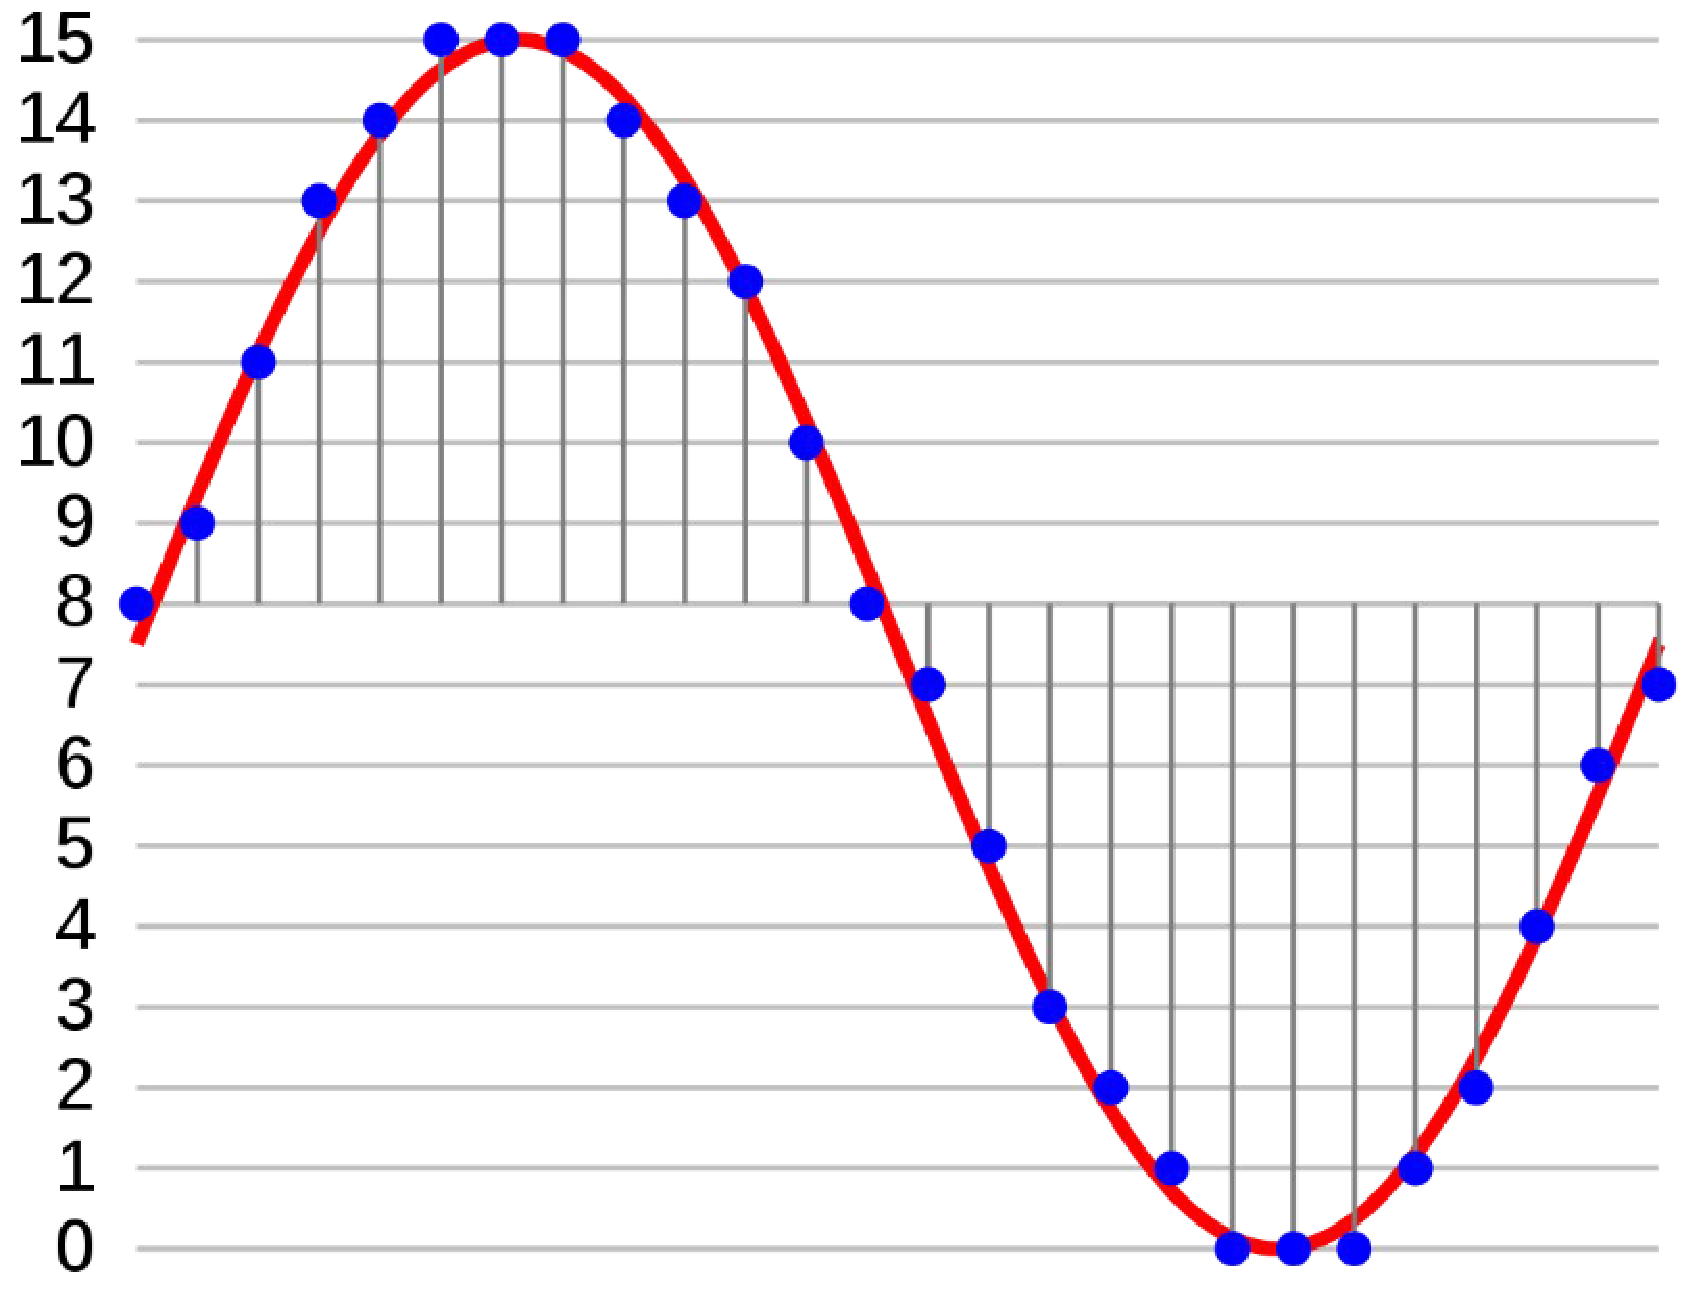
\includegraphics[width=0.7\linewidth]{img/wpan/PCM}
\end{center}

Per la voce telefonica: PCM 8bit $8000Hz$, quindi $64kbps$ (frequenza della voce $300 - 3400 Hz$). La musica viene campionata a 24bit $41/48kHz$.\\

\subsection{802.15.x}
Lo standard 802.15 comprende un insieme di tecnologie per la \textbf{comunicazione a corto raggio} (\texttt{\url{https://www.ieee802.org/15/}}).\\

Esempi di tecnologie: 
\begin{itemize}
	\item 802.15.1 Bluetooth
	\item 802.15.2 High-rate WPAN
	\item 802.15.4 Low-rate WPAN (es. Zigbee)
	\item 802.15.5 Mesh Networking (combinazione di High-rate e Low-Rate)
	\item 802.15.6 Body Area Network (BAN) pensato ad esempio per applicazioni in ambito medico
	\item 802.15.7 Visible Light Communication (VLC) (es. Vehicle-to-vehicle communication \& Li-Fi)
\end{itemize}

\subsection{Bluetooth}
Si tratta dello standard 812.15.1. Si compone di reti chiamate piconet ed all'interno della rete si ha un dispositivo \textbf{master} e \textbf{uno o più slave} sotto il controllo del master, che controlla la piconet.\\

\textbf{Caratteristiche}: 
\begin{itemize}
	\item Short range (10-50m nei casi d'uso tipici a seconda della classe di potenza del dispositivo, \texttt{\href{https://www.bluetooth.com/learn-about-bluetooth/key-attributes/range/\#estimator}{Bluetooth range estimator}})
	\item Usa la banda ISM $2.4GHz$
	\item Data Rate: $2.1 Mbps - 24Mbps$
\end{itemize}

Utilizzi: 
\begin{itemize}
	\item punto di accesso per dati e voce
	\item sostituzione di cavi (periferiche wireless)
	\item comunicazione ad hoc con altri dispositivi Bluetooth
\end{itemize}

\newpage

\subsubsection{Architettura dei protocolli} 
\begin{center}
	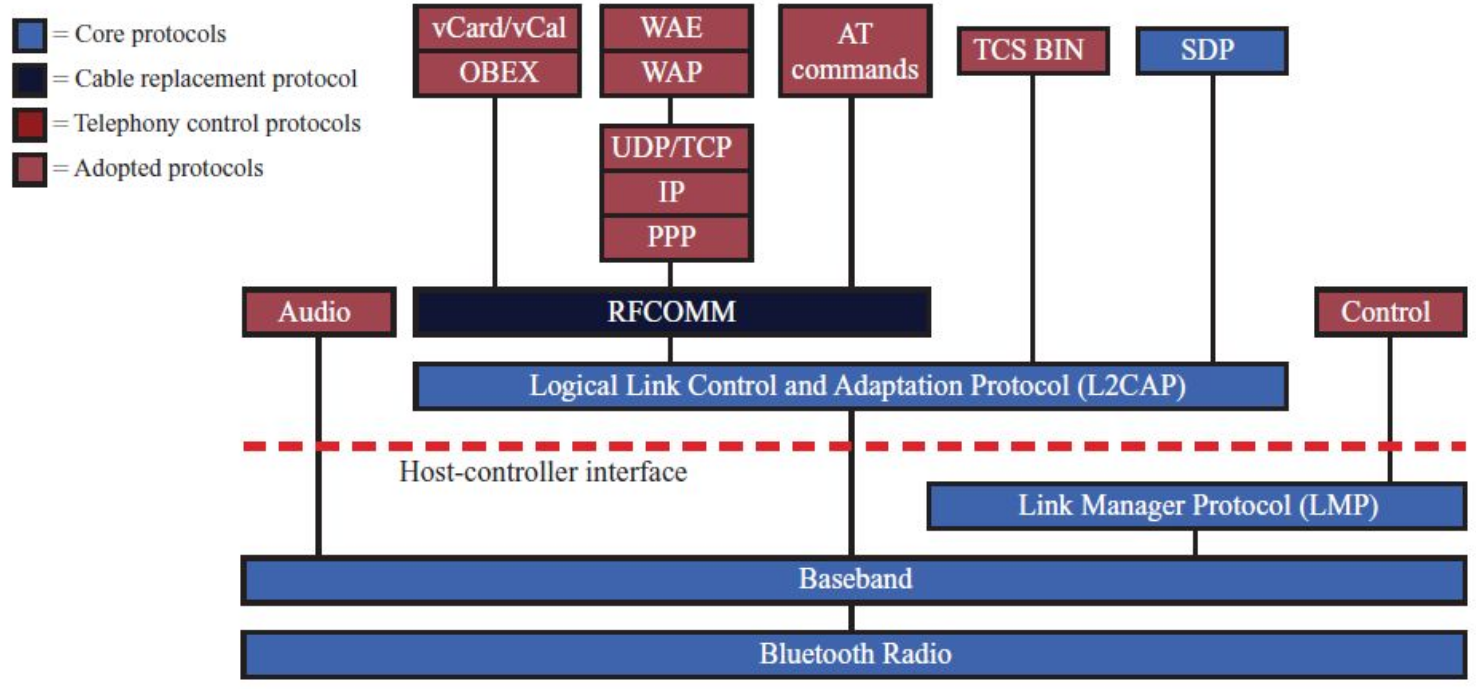
\includegraphics[width=0.95\linewidth]{img/wpan/archbt}
\end{center}
In blu sono i "core protocols", presenti in tutti i dispositivi Bluetooth. Gli altri (rossi e blu scuro) sono implementati solo se il dispositivo ne necessita, in base all'uso.\\

\paragraph{Bluetooth Radio:} La parte di livello fisico, specifica l'interfaccia radio: 
\begin{itemize}
	\item radio frequenze, quali frequenze utilizzare
	\item gestisce il frequency hopping
	\item decide lo schema di modulazioni in base al canale
	\item determina la potenza di trasmissione
\end{itemize}

\paragraph{Baseband:} Il livello di Baseband si occupa di 
\begin{itemize}
	\item stabilire la connessione con la piconet
	\item gestire l'indirizzamento
	\item formattazione dei pacchetti (frame)
	\item gestire le tempistiche di comunicazione (Time Division Duplex TDD e Time Division Multiple Access TDMA)
	\item gestisce la potenza di trasmissione (passa le indicazioni a livello radio)
\end{itemize}

\paragraph{Link Manager Protocol LMP:} Fa da "manager" del collegamento. Si occupa di:
\begin{itemize}
	\item configurare i collegamenti tra dispositivi
	\item gestione di collegamenti attivi
	\item funzionalità di sicurezza e cifratura
\end{itemize}
Si tratta di un protocollo di controllo, non passano dati ma gestisce il collegamento per i livelli sottostanti.

\paragraph{Logical Link Control and Adaptation Protocol (L2CAP):} I livelli precedenti erano implementati sul chip Bluetooth, da qui in su vengono implementati a livello software. Si occupa di:
\begin{itemize}
	\item adatta i protocolli di livello superiore al livello baseband
	\item astrarre tutto ciò che c'è sotto per i servizi a livelli superiori, \textit{Connectionless} e \textit{Connection-oriented}
\end{itemize}

\paragraph{Service Discovery Protocol SDP:} Gestisce le informazioni del dispositivo. Permette di comunicare
\begin{itemize}
	\item servizi disponibili sul dispositivo
	\item caratteristiche sul dispositivi
\end{itemize}
Stile architettura client-server: prevede interrogazioni richiesta-risposta per stabilire connessioni tra dispositivi Bluetooth.

\paragraph{Radio Frequency Communication RFCOMM:} Astrae il livello di Bluetooth, permette di "astrarre un cavo". Simula una comunicazione seriale e permette la trasmissione di dati tra dispositivi Bluetooth.

\paragraph{Livelli superiori:} I livelli in rosso sono protocolli "già esistenti", ciascun dispositivo può avere parte di questi protocolli in base all'uso, i livelli inferiori permettono la comunicazione a livello fisico.\\

\newpage

\paragraph{Profili:} Per avere determinate funzionalità un dispositivo deve seguire dei "profili". Esempi di profili:
\begin{center}
	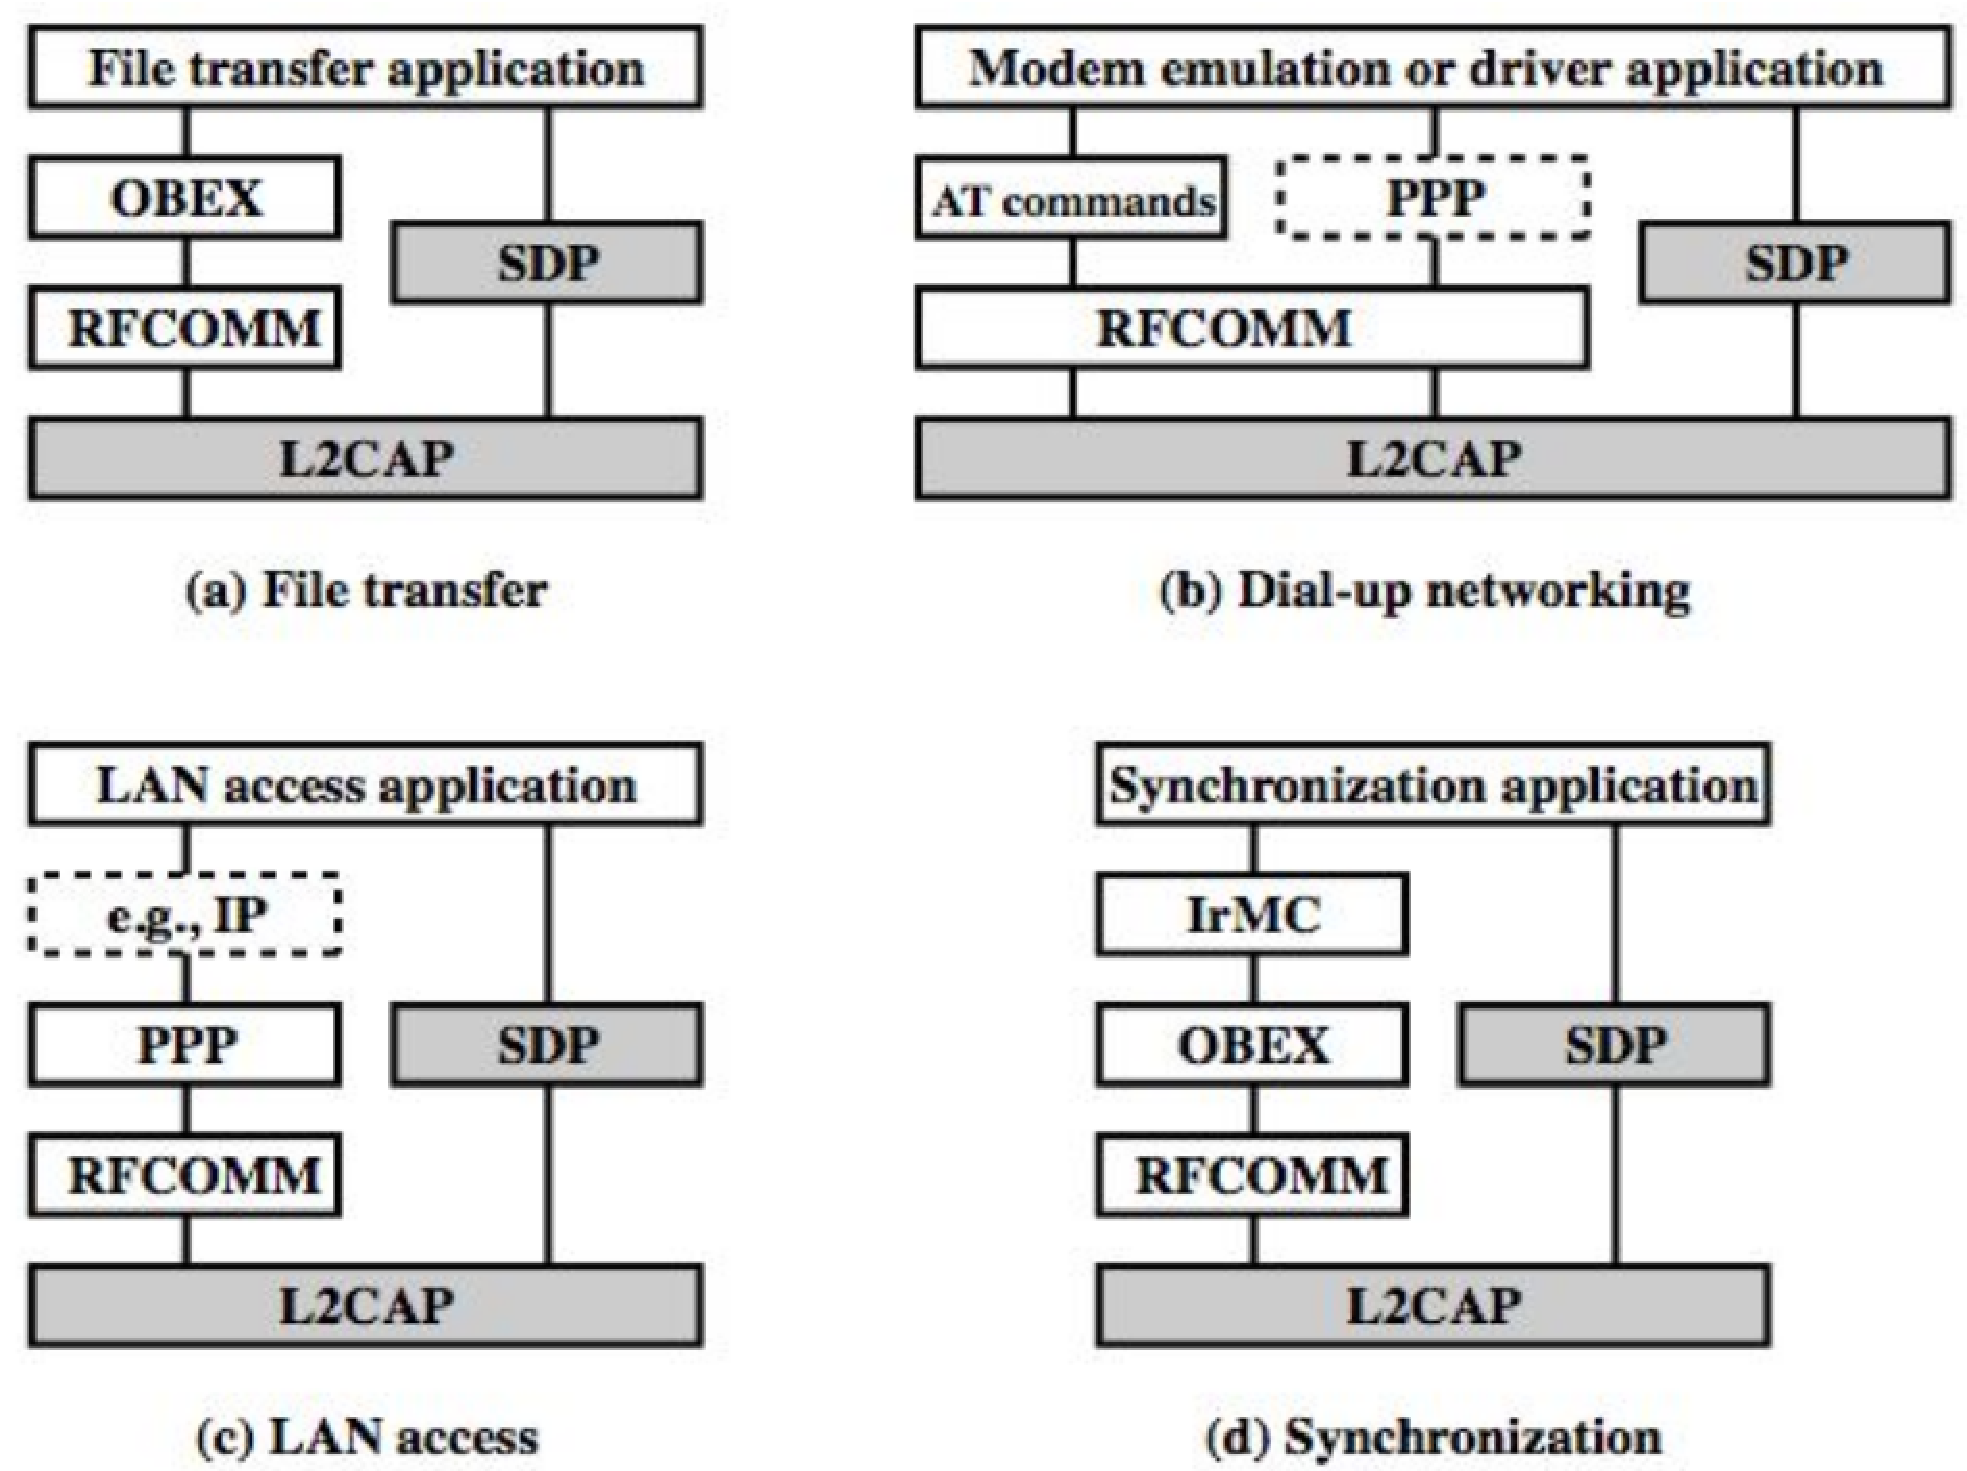
\includegraphics[width=0.7\linewidth]{img/wpan/profiles}
\end{center}
Questi sono standard, un dispositivo deve aderire ad uno o più profili (annunciati dal SDP) per avere il relativo utilizzo.\\

\newpage

\subsubsection{Piconet \& Scatternet}

\paragraph{Piconet:} Una piconet è composta da un \textbf{master} e 
\begin{itemize}
	\item \textbf{Active Slave (AS)}: membro attivo delle piconet, con un indirizzo Active Member Address (AMA) su 3 bit assegnato dal master (0 è il master, quindi 7 dispositivi al massimo)
	\item \textbf{Parked Slave (PS)}: membro della piconet ma temporaneamente disattivato, non possono comunicare attivamente ma solo ogni tanto tramite il Parked Member Address (PMA), 8 bit (0 è il master); un parked può tornare attivo solo se "c'è spazio"
	\item \textbf{Standby Slave (SS)}: non sconosciuti ma scollegati; non hanno indirizzi e possono quindi essere infiniti
\end{itemize}
\begin{center}
	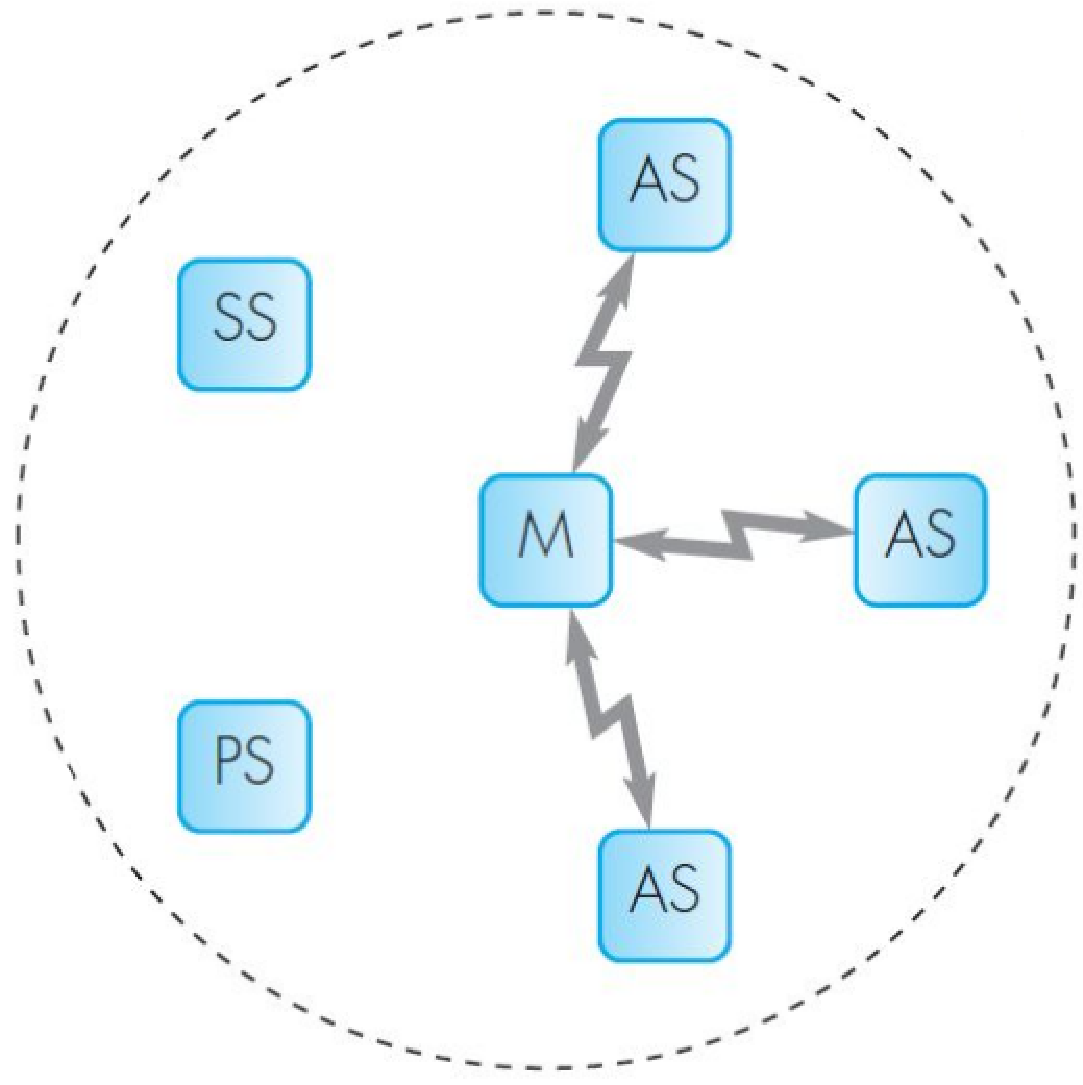
\includegraphics[width=0.35\linewidth]{img/wpan/pico1}
\end{center}

\paragraph{Scatternet:} La piconet ha al centro sempre un master, ma un dispositivo può appartenere a più piconet, portando ad una scatternet
\begin{center}
	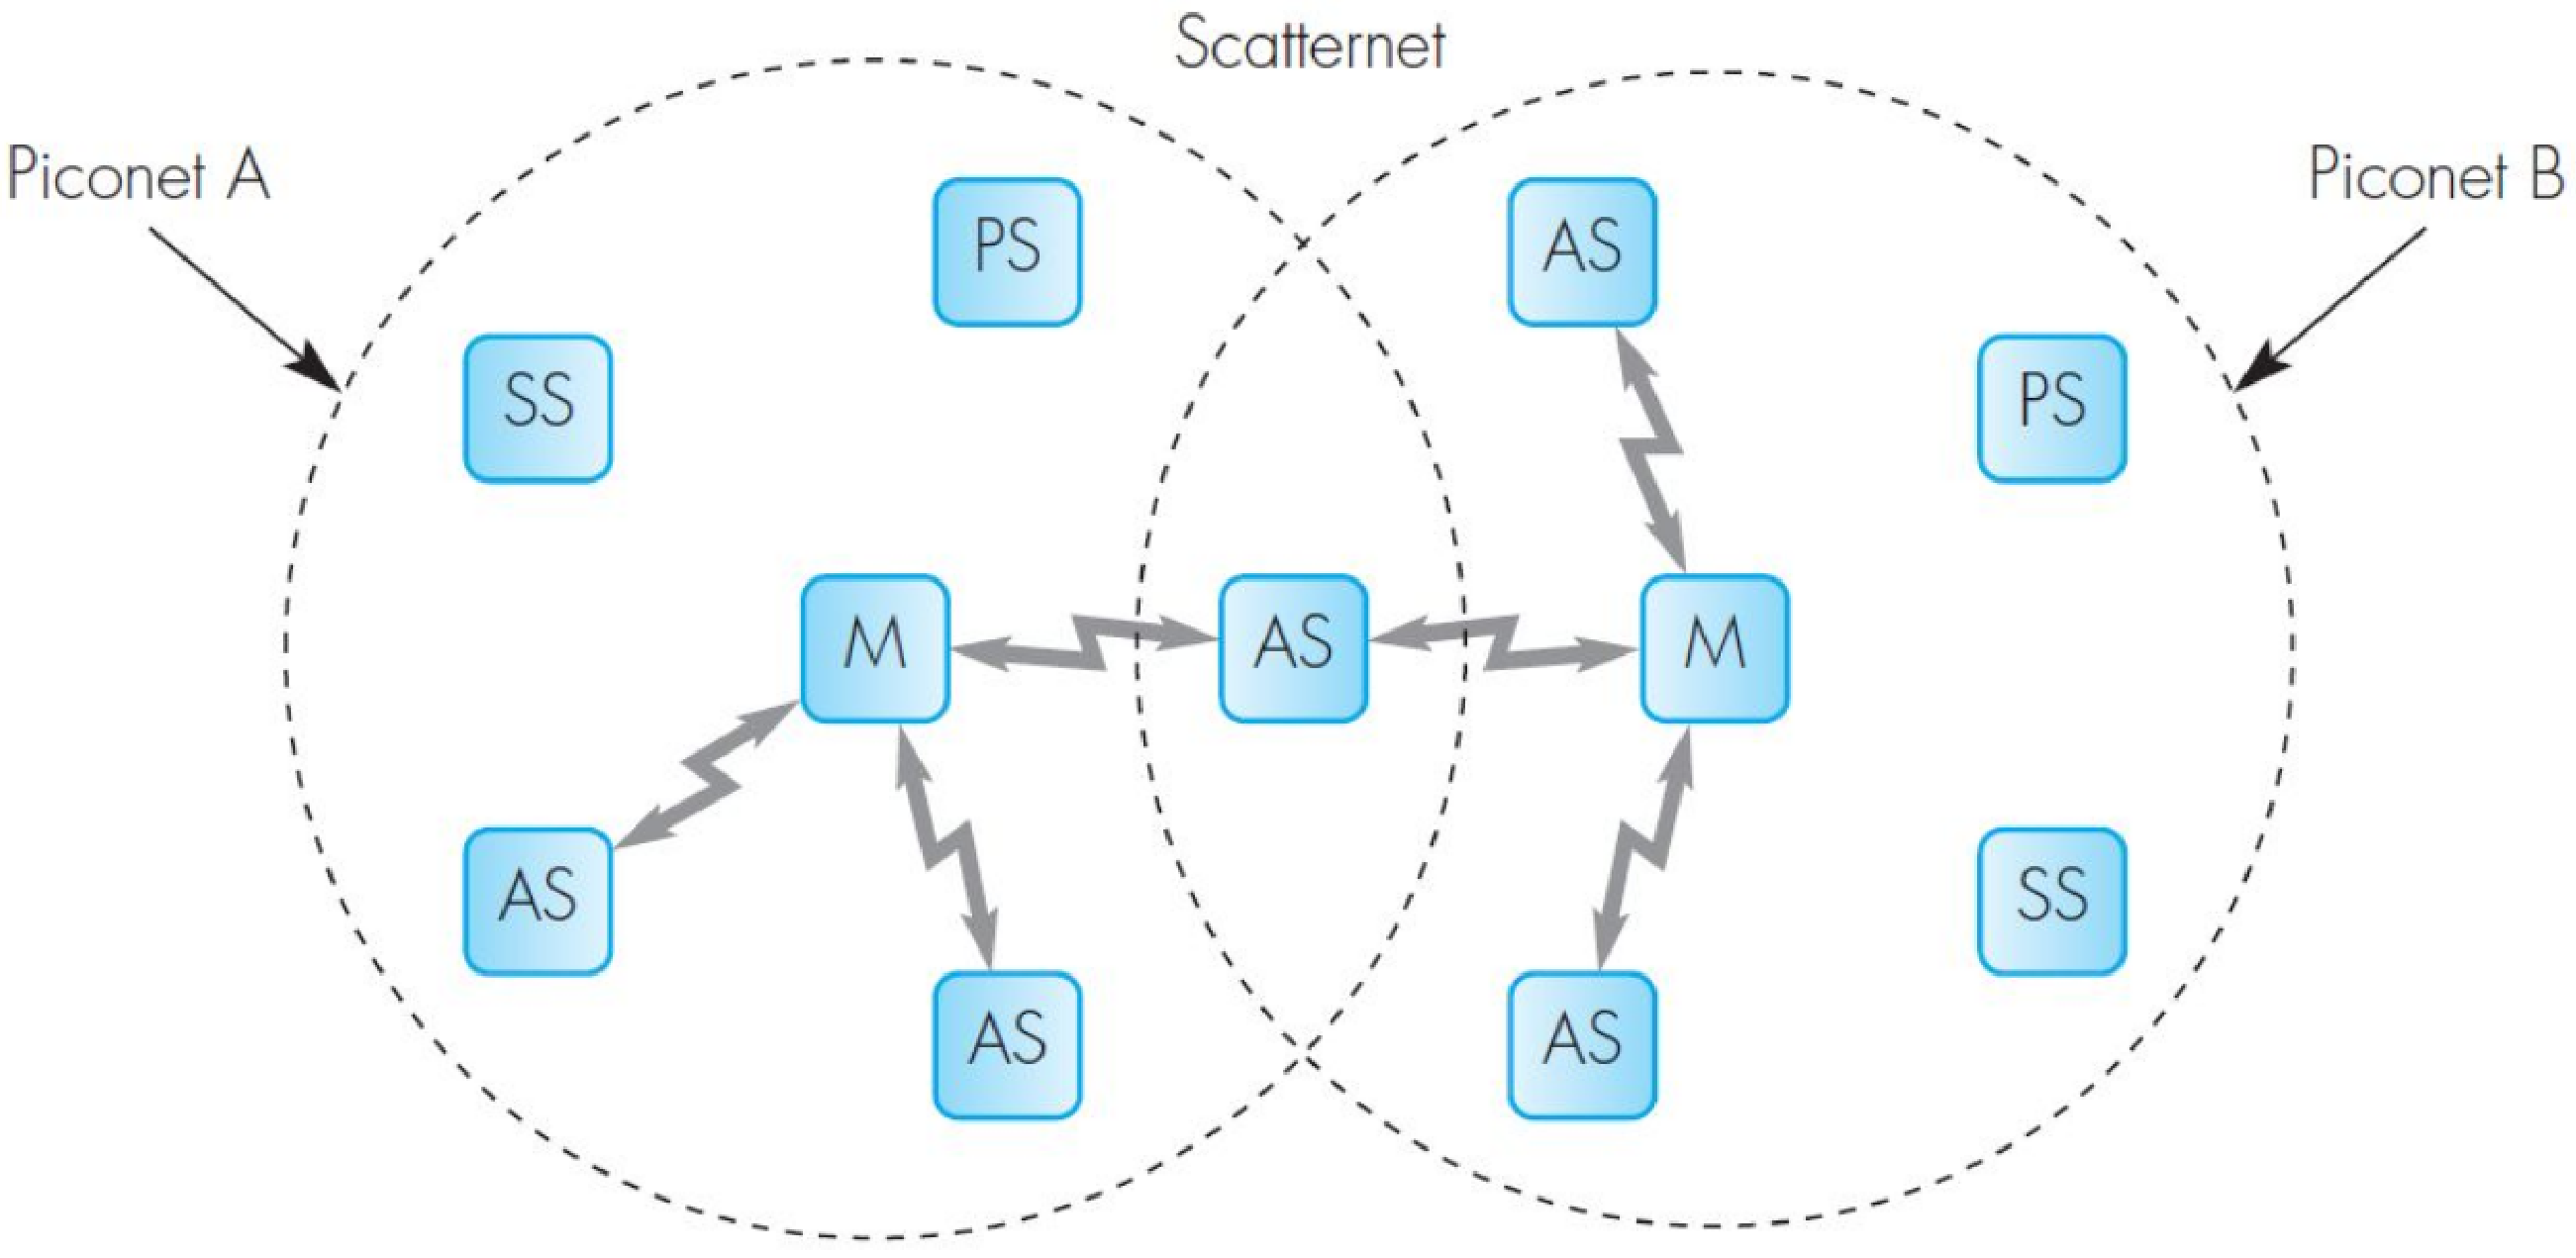
\includegraphics[width=0.7\linewidth]{img/wpan/scatter}
\end{center}
In qualsiasi caso i master lavorano in maniera completamente \textbf{separata}. Un AS attivo in due piconet diverse avrà indirizzamento diverso sulle due reti.

\subsubsection{Bluetooth Radio}
\paragraph{Specifiche radio Bluetooth 2.1:}
\begin{center}
	{
	\resizebox{0.98\textwidth}{!}{
	\renewcommand{\arraystretch}{1.2}
	\begin{tabular}{|l|l|l|}
		\hline
		& \textbf{Basic Rate (BR)} & \textbf{Enhanced Data Rate (EDR)} \\ 
		\hline
		\textbf{Topology} & \multicolumn{2}{c|}{Up to 7 simultaneous links in a logical star} \\ 
		\hline
		\textbf{Modulation} & GFSK & $\pi/4$-DQPSK and 8DPSK \\ 
		\hline
		\textbf{Peak data rate} & $1 Mbps$ & $2 Mbps$ and $3 Mbps$ \\ 
		\hline
		\textbf{RF bandwidth} & \multicolumn{2}{c|}{$220 kHz (-3 dB)$, $1 MHz (-20 dB)$} \\ 
		\hline
		\textbf{RF band} & \multicolumn{2}{c|}{$2.4 GHz$, ISM band} \\ 
		\hline
		\textbf{RF carriers} &  \multicolumn{2}{c|}{$23/79$}  \\ 
		\hline
		\textbf{Carrier spacing} &  \multicolumn{2}{c|}{$1MHz$}  \\ 
		\hline
		\textbf{Transmit power} &  \multicolumn{2}{c|}{$0.1W$}  \\ 
		\hline
		\textbf{Piconet access} &  \multicolumn{2}{c|}{FH-TDD-TDMA} \\ 
		\hline
		\textbf{Frequency hop rate} & \multicolumn{2}{c|}{1600 hops/s}\\ 
		\hline
		\textbf{Scatternet access} & \multicolumn{2}{c|}{FH-CDMA} \\ 
		\hline
	\end{tabular}}
	}
\end{center}
Per gestire le scatternet si usa FH-CDMA, anche in caso due scatternet comunichino sulla stessa frequenza si usa CDMA per poter distinguere i segnali.\\

\paragraph{Classi di potenza:} I dispositivi Bluetooth si differenziano in base alla classe di potenza
\begin{itemize}
	\item Power class 1: $100 mW$ 100 metri (senza ostacoli)
	\item Power class 2: $2.5 mW$ 10 metri (più tipico per BT)
	\item Power class 3: $1 mW$ 1-2 metri
\end{itemize}

\newpage

\paragraph{Comunicazione nelle piconet:} All'interno di una piconet vengono usate
\begin{itemize}
	\item Frequency Hopping FH: la frequenza è decisa dal master e condivisa agli slave nella piconet
	\item Time Division Duplex TDD: la comunicazione tra master e slave è gestita in tempo e alternata, prima comunica il master con lo slave, poi si invertono, con slot di $625\mu s$ (inclusa una guardia di $220 \mu s$)
	\item Time Division Multiple Access TDMA: per gestire più dispositivi nello stesso momento
\end{itemize}
\begin{center}
	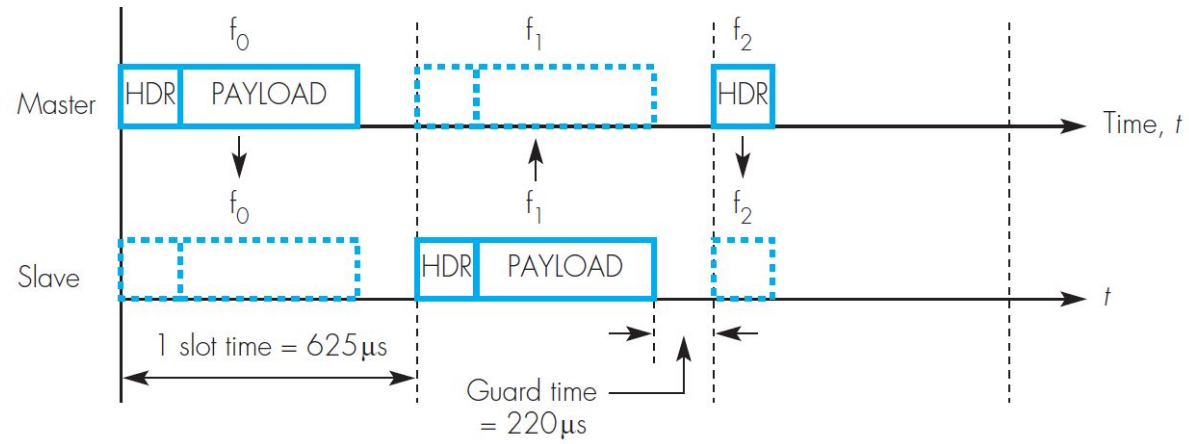
\includegraphics[width=0.9\linewidth]{img/wpan/picocomm}
\end{center}

%End L5

Esempio a più dispositivi: 
\begin{center}
	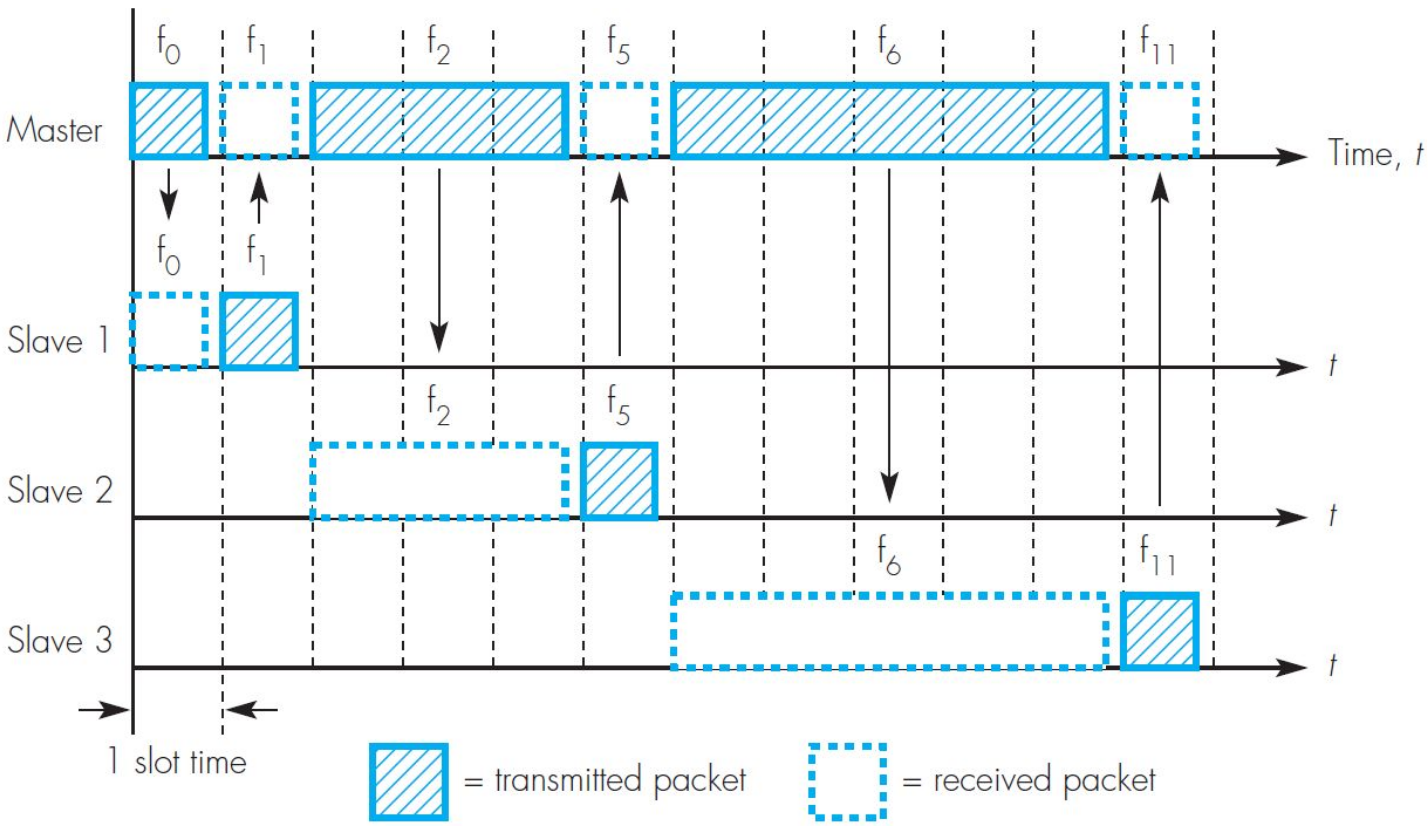
\includegraphics[width=0.9\linewidth]{img/wpan/picocomm2}
\end{center}

Nelle frequenze pari master a slave, nelle frequenze dispari viceversa. Più slave vengono coordinati tramite TDMA, ovvero il master decide chi parla in quale slot di tempo. La \textbf{dimensione dei messaggi} può essere di 1, 3 o 5 slot di tempo consecutivi (dispari per mantenere l'alternanza in TDD). Nell'header di ogni pacchetto c'è la dimensione.\\

La frequenza usata dal frequency hopping è data dal numero di timeslot passati, non dal numero di messaggi, quindi al time slot 5 viene usata la quinta frequenza $f_5$, anche se sono stati inviati solo 3 messaggi. Per una singola trasmissione (messaggio) viene mantenuta la stessa frequenza (non cambia a metà). All'interno della piconet tutti i clock devono essere sincronizzati.\\

\paragraph{Scatternet:} Nel caso di una scatternet, ogni piconet che la compone ha tutto diverso: diverse frequenze, diverso clock e di conseguenza completa autonomia. Un AS connesso a più piconet deve essere in grado di gestire le due connessioni indipendentemente.\\

Su 79 canali, cambiati ogni $625 \mu s$, può capitare una sovrapposizione (quindi interferenza), possibili soluzioni sono: 
\begin{itemize}
	\item FH su un numero ridotto di canali, e.g., ogni piconet su 20 canali e si spera non ci sia sovrapposizione in quei 20
	\item Si usa CDMA per evitare interferenze; il master comunica un codice ortogonale ai dispositivi all'interno della piconet (soluzione usata)
\end{itemize}

\newpage

\subsubsection{Baseband}

\paragraph{Tipologie di servizio:} Offre due possibili canali logici: 
\begin{itemize}
	\item \textbf{Synchronous Connection-Oriented Link (SCO)} point-to-point:
	\begin{itemize}
		\item canale audio/voce di $64kbps$ bidirezionale
		\item il master riserva una coppia di slot adiacenti ad intervalli regolari
		\item previsti fino al massimo di 3 canali SCO attivi contemporaneamente
		\item traffico real time
	\end{itemize}
	Garantiscono un bit rate fisso, un canale riservato, usato per casistiche sensibili al delay (real time).
	
	\item \textbf{Asynchronous Connectionless Link (ACL)} point-to-multipoint:
	\begin{itemize}
		\item canali ACL occupano gli slot rimanenti
		\item traffico dati con ciascuno degli slave
		\item un solo ACL contemporaneo fra master e uno slave
		\item traffico best effort (nessuna garanzia di delay)
	\end{itemize}
	Bit rate non costante, permette una qualità maggiore ma senza nessuna garanzia.
\end{itemize}
\begin{center}
	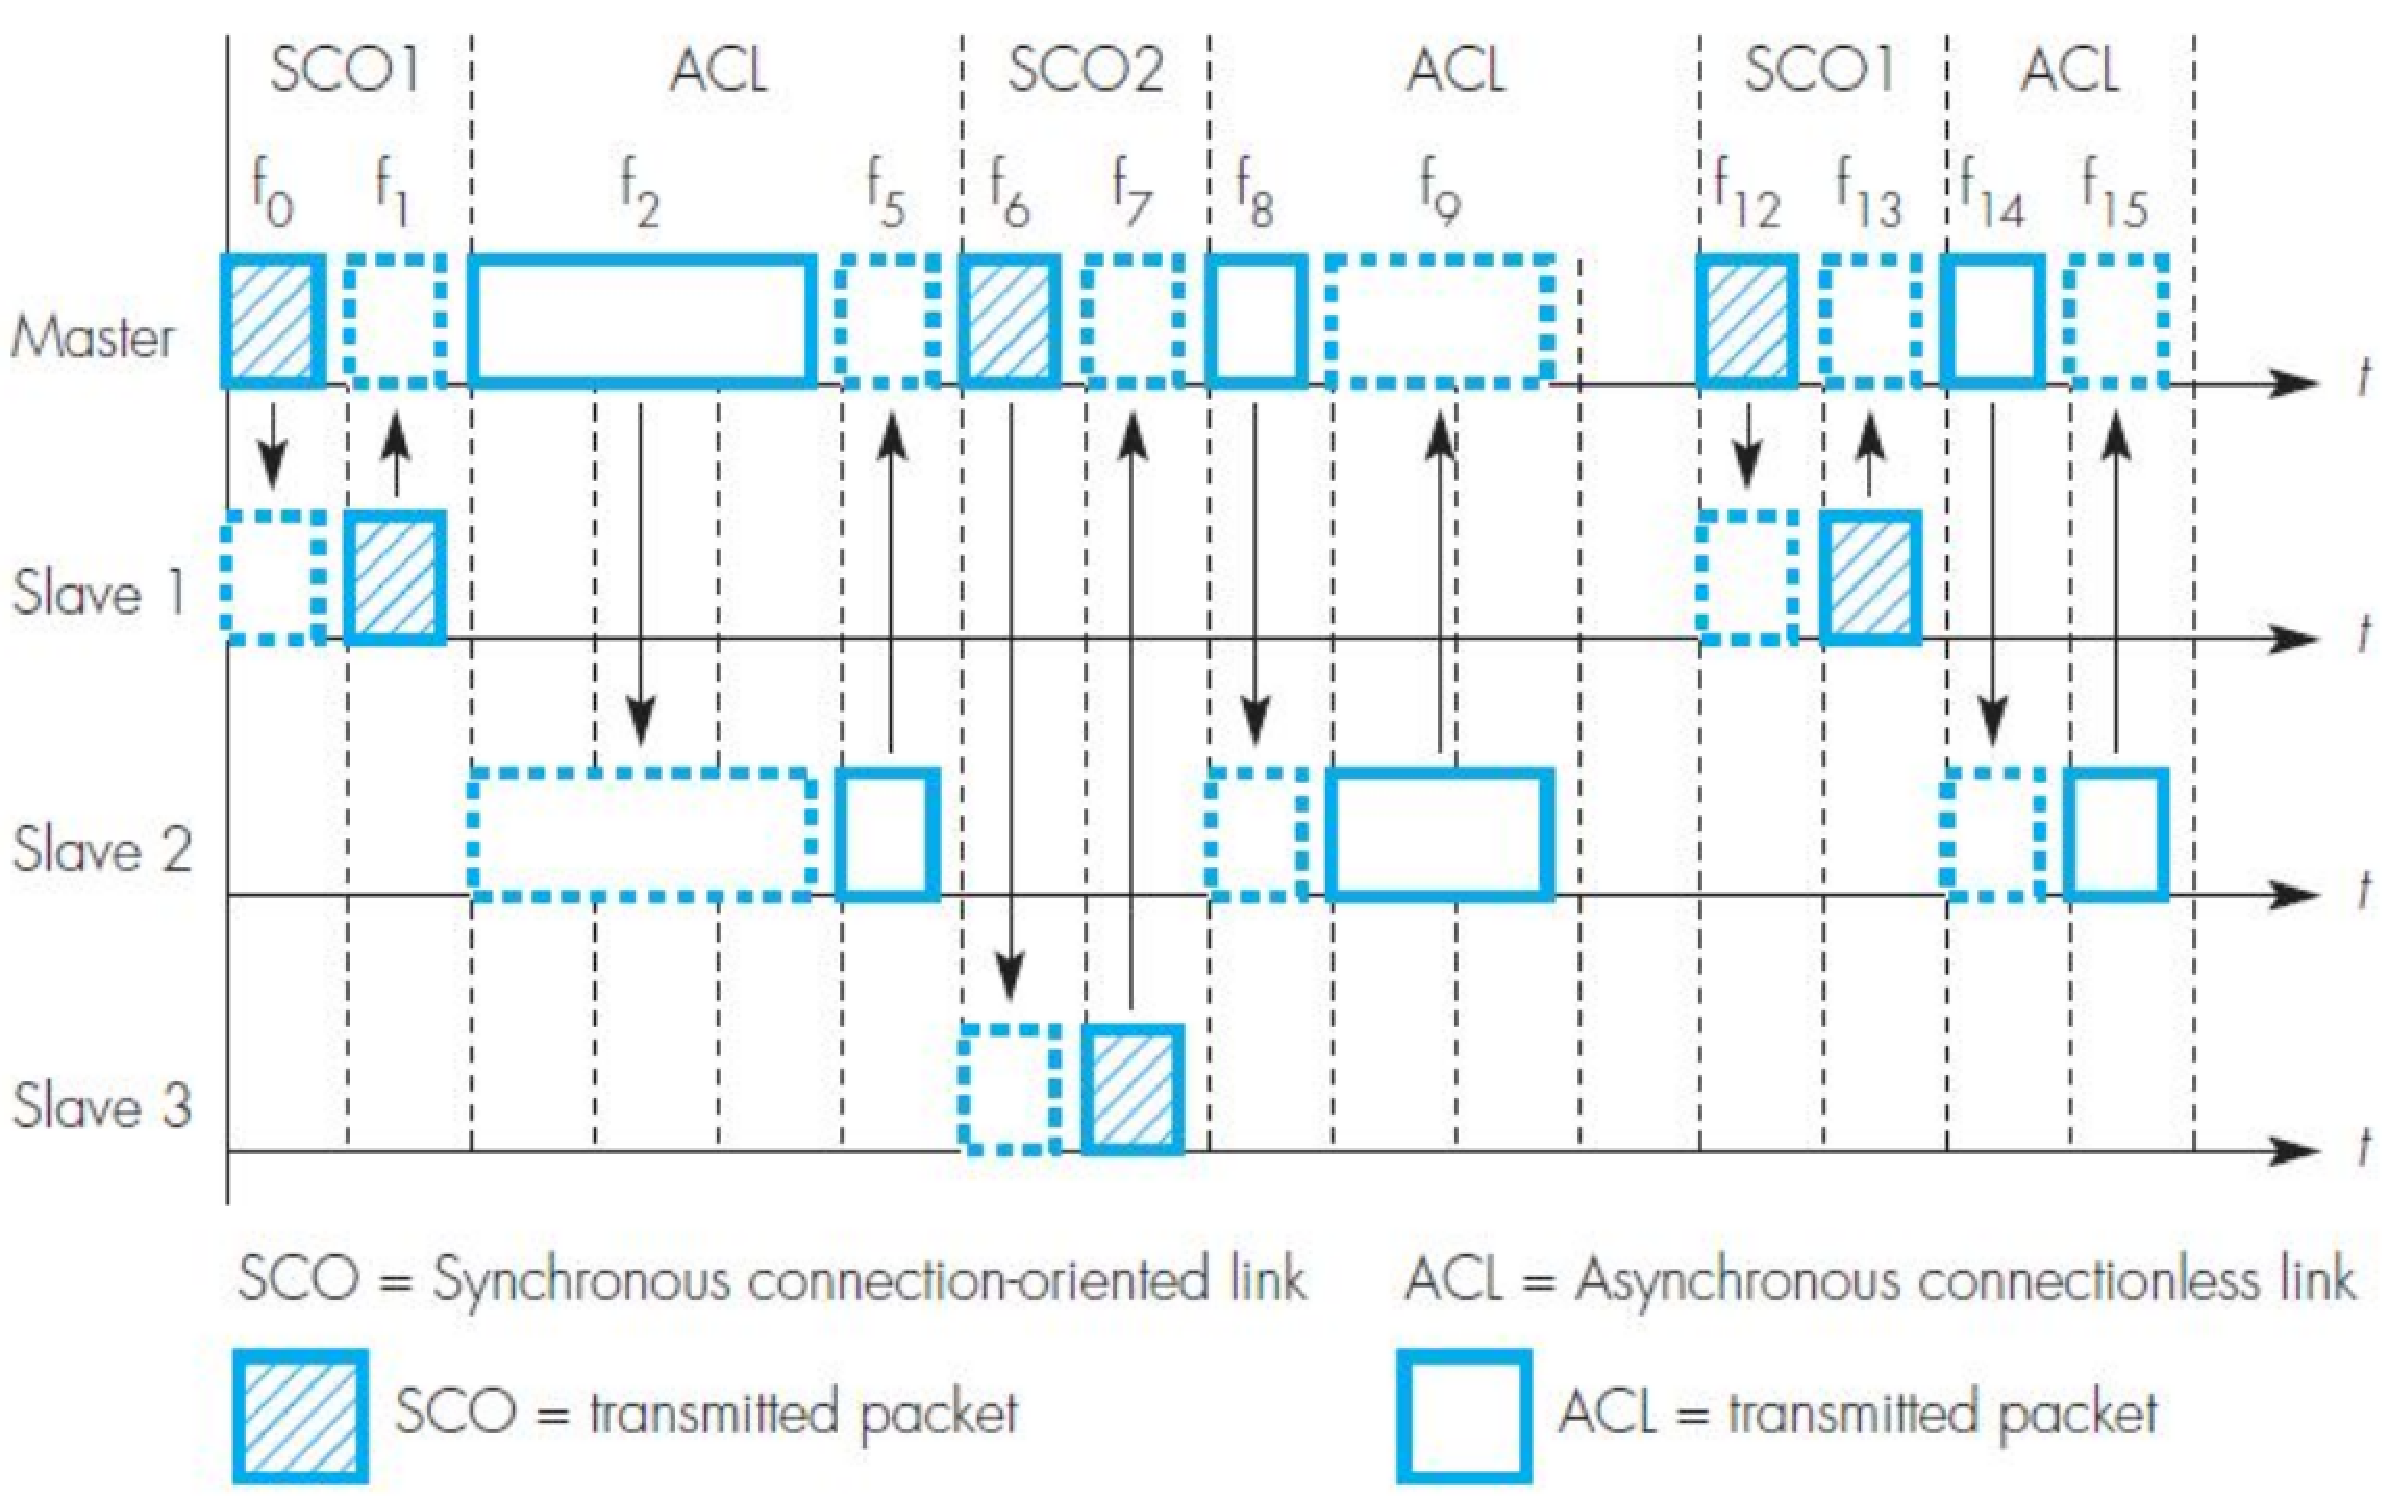
\includegraphics[width=0.9\linewidth]{img/wpan/scoacl}
\end{center}

\paragraph{Formato pacchetti:} 
\begin{center}
	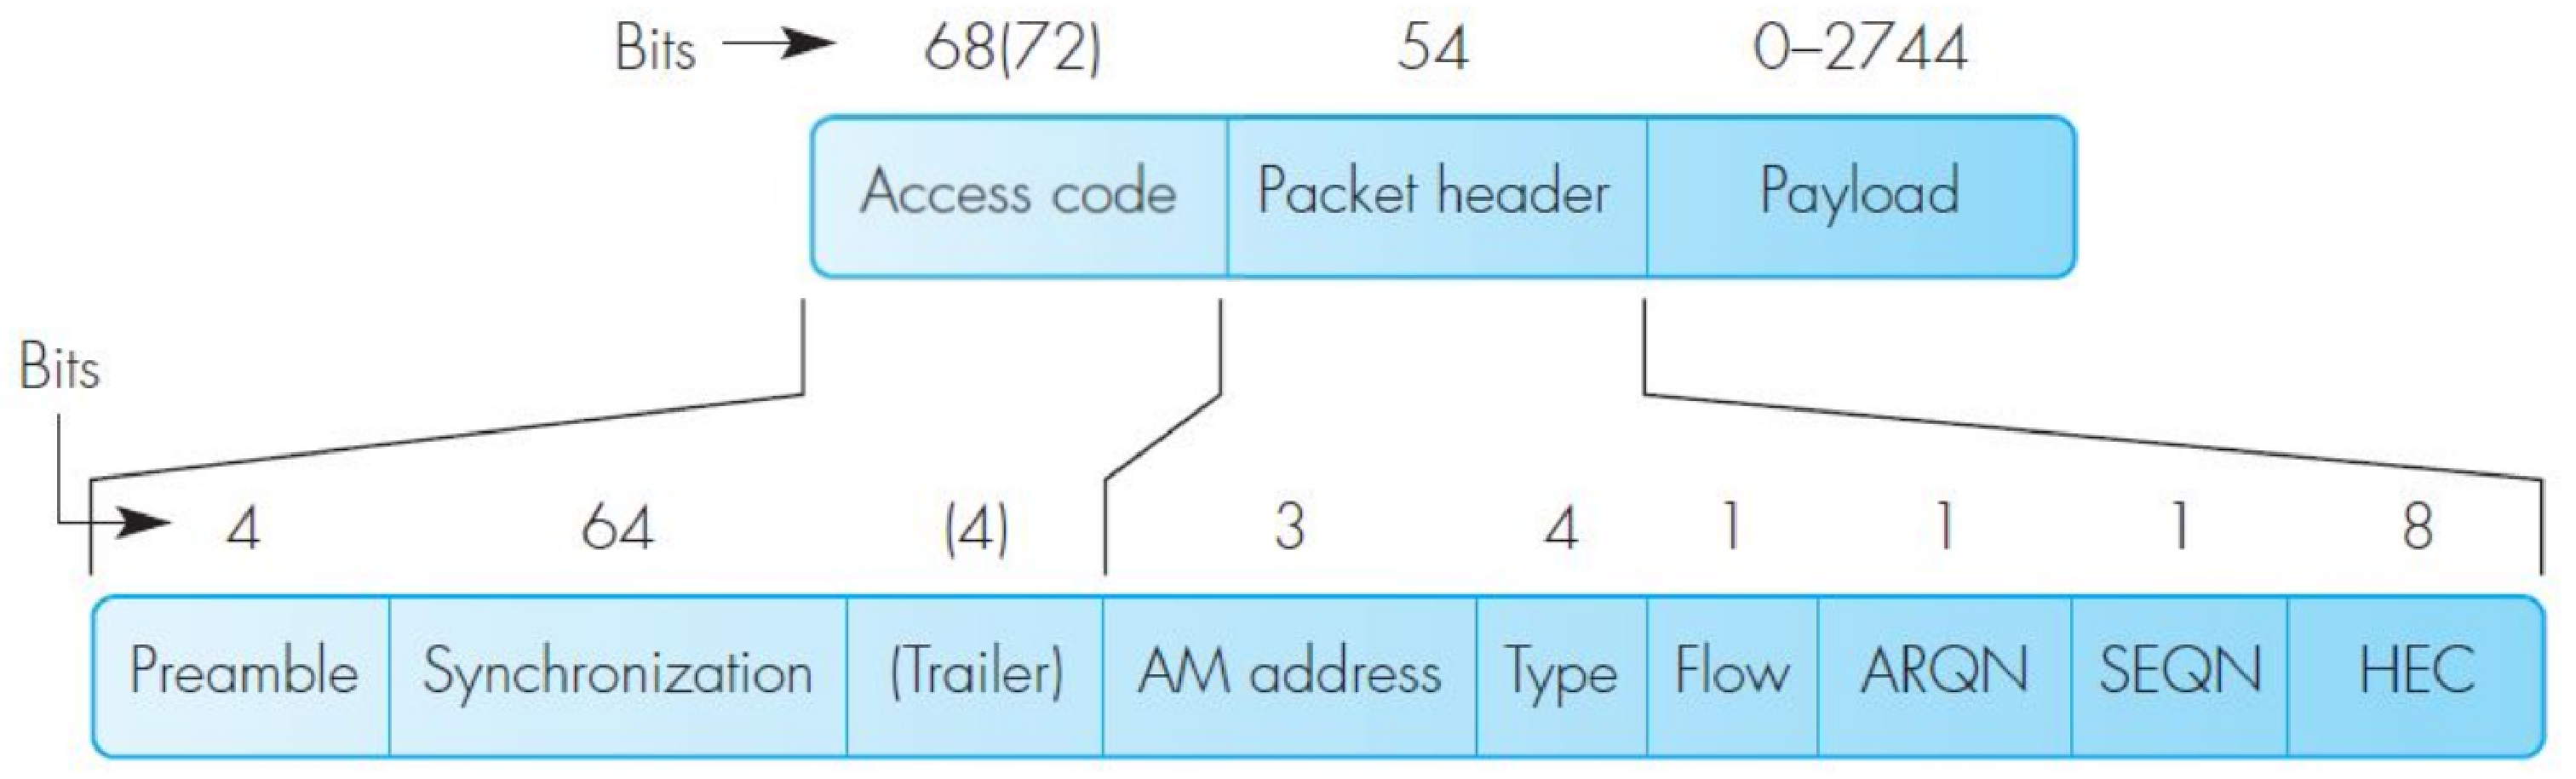
\includegraphics[width=0.9\linewidth]{img/wpan/basebandpacket}
\end{center}
Access code: utilizzato per sincronizzazione e identificazione. Può essere di 3 tipi:
\begin{itemize}
	\item Channel Access Code (CAC): identifica la piconet (derivato dai 48 bit dell'indirizzo hardware del master)
	\item Device Address Code (DAC): derivato dall'indirizzo hardware dello slave ed è usato dal master per chiamare il dispositivo (paging)
	\item Inquiry Address Code (IAC): usato per trovare l'indirizzo di un dispositivo vicino (durante la fase di inquiry)
\end{itemize}

Packet Header: ha diversi campi: 
\begin{center}
	    \begin{tabular}{|l|p{10cm}|}
		\hline
		\textbf{Campo Header} & \\ \hline
		AMA & Indirizzo del membro attivo della piconet \\ \hline
		Type & Identifica la tipologia del pacchetto e il formato del pacchetto SCO/ACL, numero di slot ecc... \\ \hline
		Flow & Per gli ACL: stop (1), resume (0) \\ \hline
		ARQN & 1 ACK, 0 NACK \\ \hline
		SEQN & Sequence number modulo 2 \\ \hline
		HEC & Controllo errori del campo header (1/3 FEC) \\ \hline
	\end{tabular}
\end{center}
ARQN e SEQN sono 2 bit necessari e sufficienti per il controllo degli errori (bastano grazie alla rigida struttura di comunicazione delineala al livello precedente).\\

%TODO Wtf, idk
Payload: contenuto effettivo del pacchetto può essere: 
\begin{itemize}
	\item SCO: 30 byte,  (FEC 0, 2/3, 1/3), che porta a massimo $64kbps$, dato che $(30 \cdot 8) \cdot (1600/6)$, ovvero $30 \cdot 8$ bit, 
	\item ACL: variabile da 0 a 343 byte
\end{itemize}

\paragraph{Controllo degli errori: }
\begin{center}
	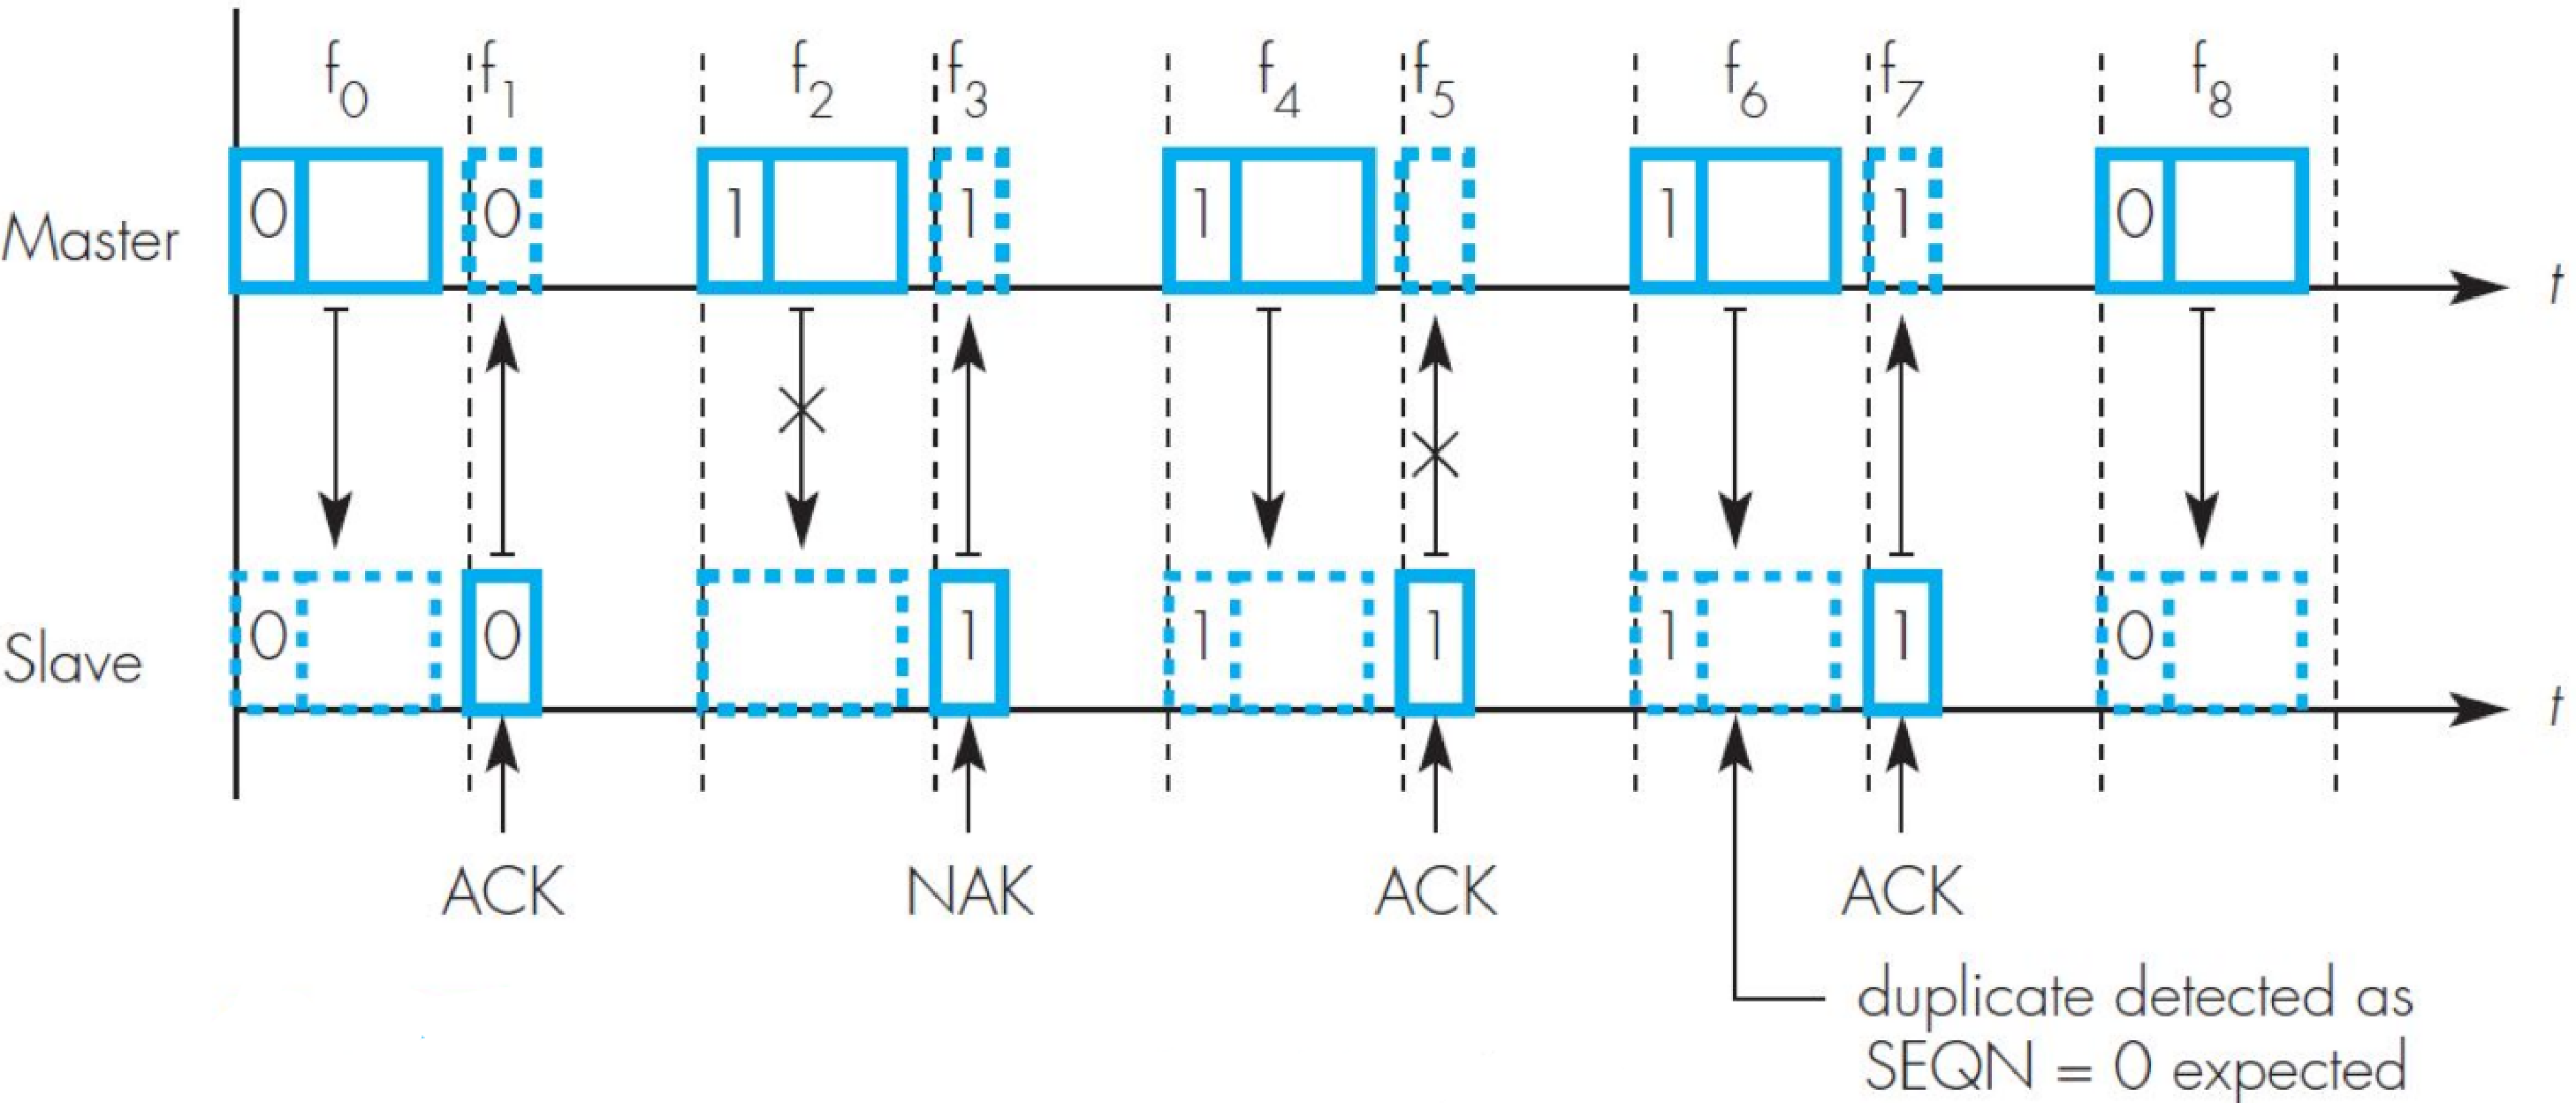
\includegraphics[width=0.9\linewidth]{img/wpan/errorcorr1}
\end{center}

All'interno del quadrato blu si vede il SEQN, mentre ACK/NACK sono indicati al di fuori.\\

Sequenza tipica:
\begin{itemize}
	\item Il master invia un pacchetto con un SEQN $s$
	\item lo slave risponde con un ACK ed un SEQN $s$ (lo stesso)
\end{itemize}

Possibili problemi: 
\begin{itemize}
	\item Lo slave non riceve il pacchetto: invierà un NACK per indicare la mancata ricezione, nello slot successivo deve parlare lo stesso dato che "è il suo turno", sa che ci sarà un SEQN pari a $\neg s$ ma non ha ricevuto nulla e lo indica con il NACK. "Non ho ricevuto e mi aspettavo questo"
	\item Se il master non riceve risposta dallo slave (ACK perso), il pacchetto viene re-inviato, con la possibilità di inviare un duplicato, ma meglio che perdere pacchetti
	\item Lo slave riceve un duplicato e se ne accorge in quanto il SEQN è uguale a quello precedente (il master non ha ricevuto l'ACK, non è cambiato il SEQN, quindi è una ritrasmissione del pacchetto precedente)
\end{itemize}
La rigidità dell'alternanza tra master e slave permette di rendere minimale lo spazio necessario per effettuare il controllo degli errori.\\

\newpage

\subsubsection{Link Manager Protocol}
\paragraph{Transizioni di stato:}
\begin{center}
	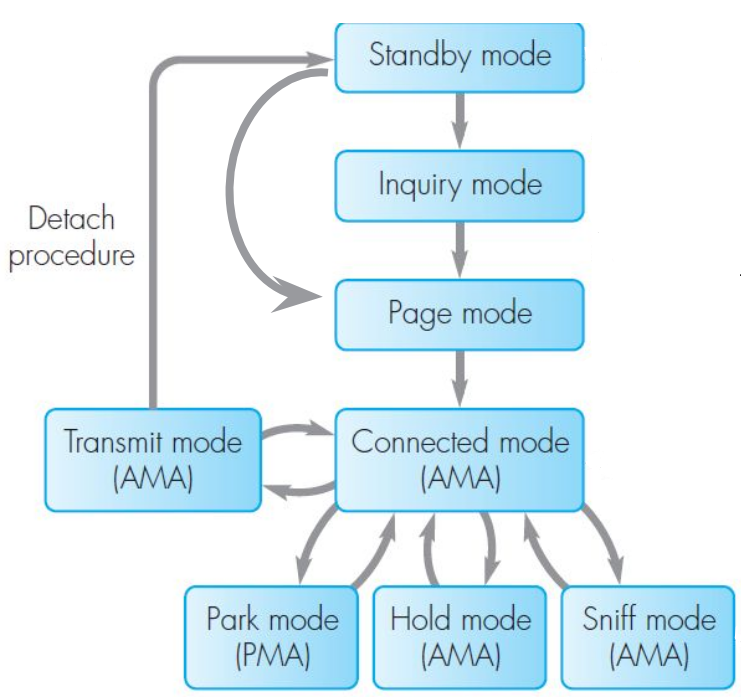
\includegraphics[width=0.55\linewidth]{img/wpan/lmpst}
\end{center}

\paragraph{Standby Mode:} A dispositivo "appena acceso" entra in standby mode, non membro di alcuna piconet, minimo consumo.\\

\paragraph{Enquiry mode:} Periodicamente il master invia 32 messaggi consecutivi usando 32 canali (wake-up channels, la sequenza  è standard). I messaggi contengono un \textbf{IAC packet}. Gli slave periodicamente ascoltano i 32 canali per vedere se qualcuno ha mandato un IAC packet. Tutto questo in modo non coordinato.\\

Ogni dispositivo ascolta per $11,25 ms$, all'inizio di ogni intervallo di $1,28$ o $2,56 s$. Una volta "beccata" una trasmissione del master si aspetta un numero random di slot di tempo (random backoff) prima di trasmettere la risposta (per evitare che più slave che hanno ascoltato quella trasmissione rispondano nello stesso momento). Possiamo farlo dato che adesso l'unica cosa che sappiamo è il clock del master, ricevere un qualsiasi segnale del master permette di sincronizzarsi con la piconet. La risposta contiene il Blouetooth Device Address dello slave e la classe, per indicare il tipo di dispositivo.\\

\newpage

Per finalizzare la connessione mancano le frequenze di hopping: si usano 16 delle 32 frequenze standard, per mandare: Device Access Code DAC, la sequenza di FH e l'Active Member Address AMA dello slave.\\

Lo slave risponde con DAC e ACK, poi può cominciare la comunicazione.
\begin{center}
	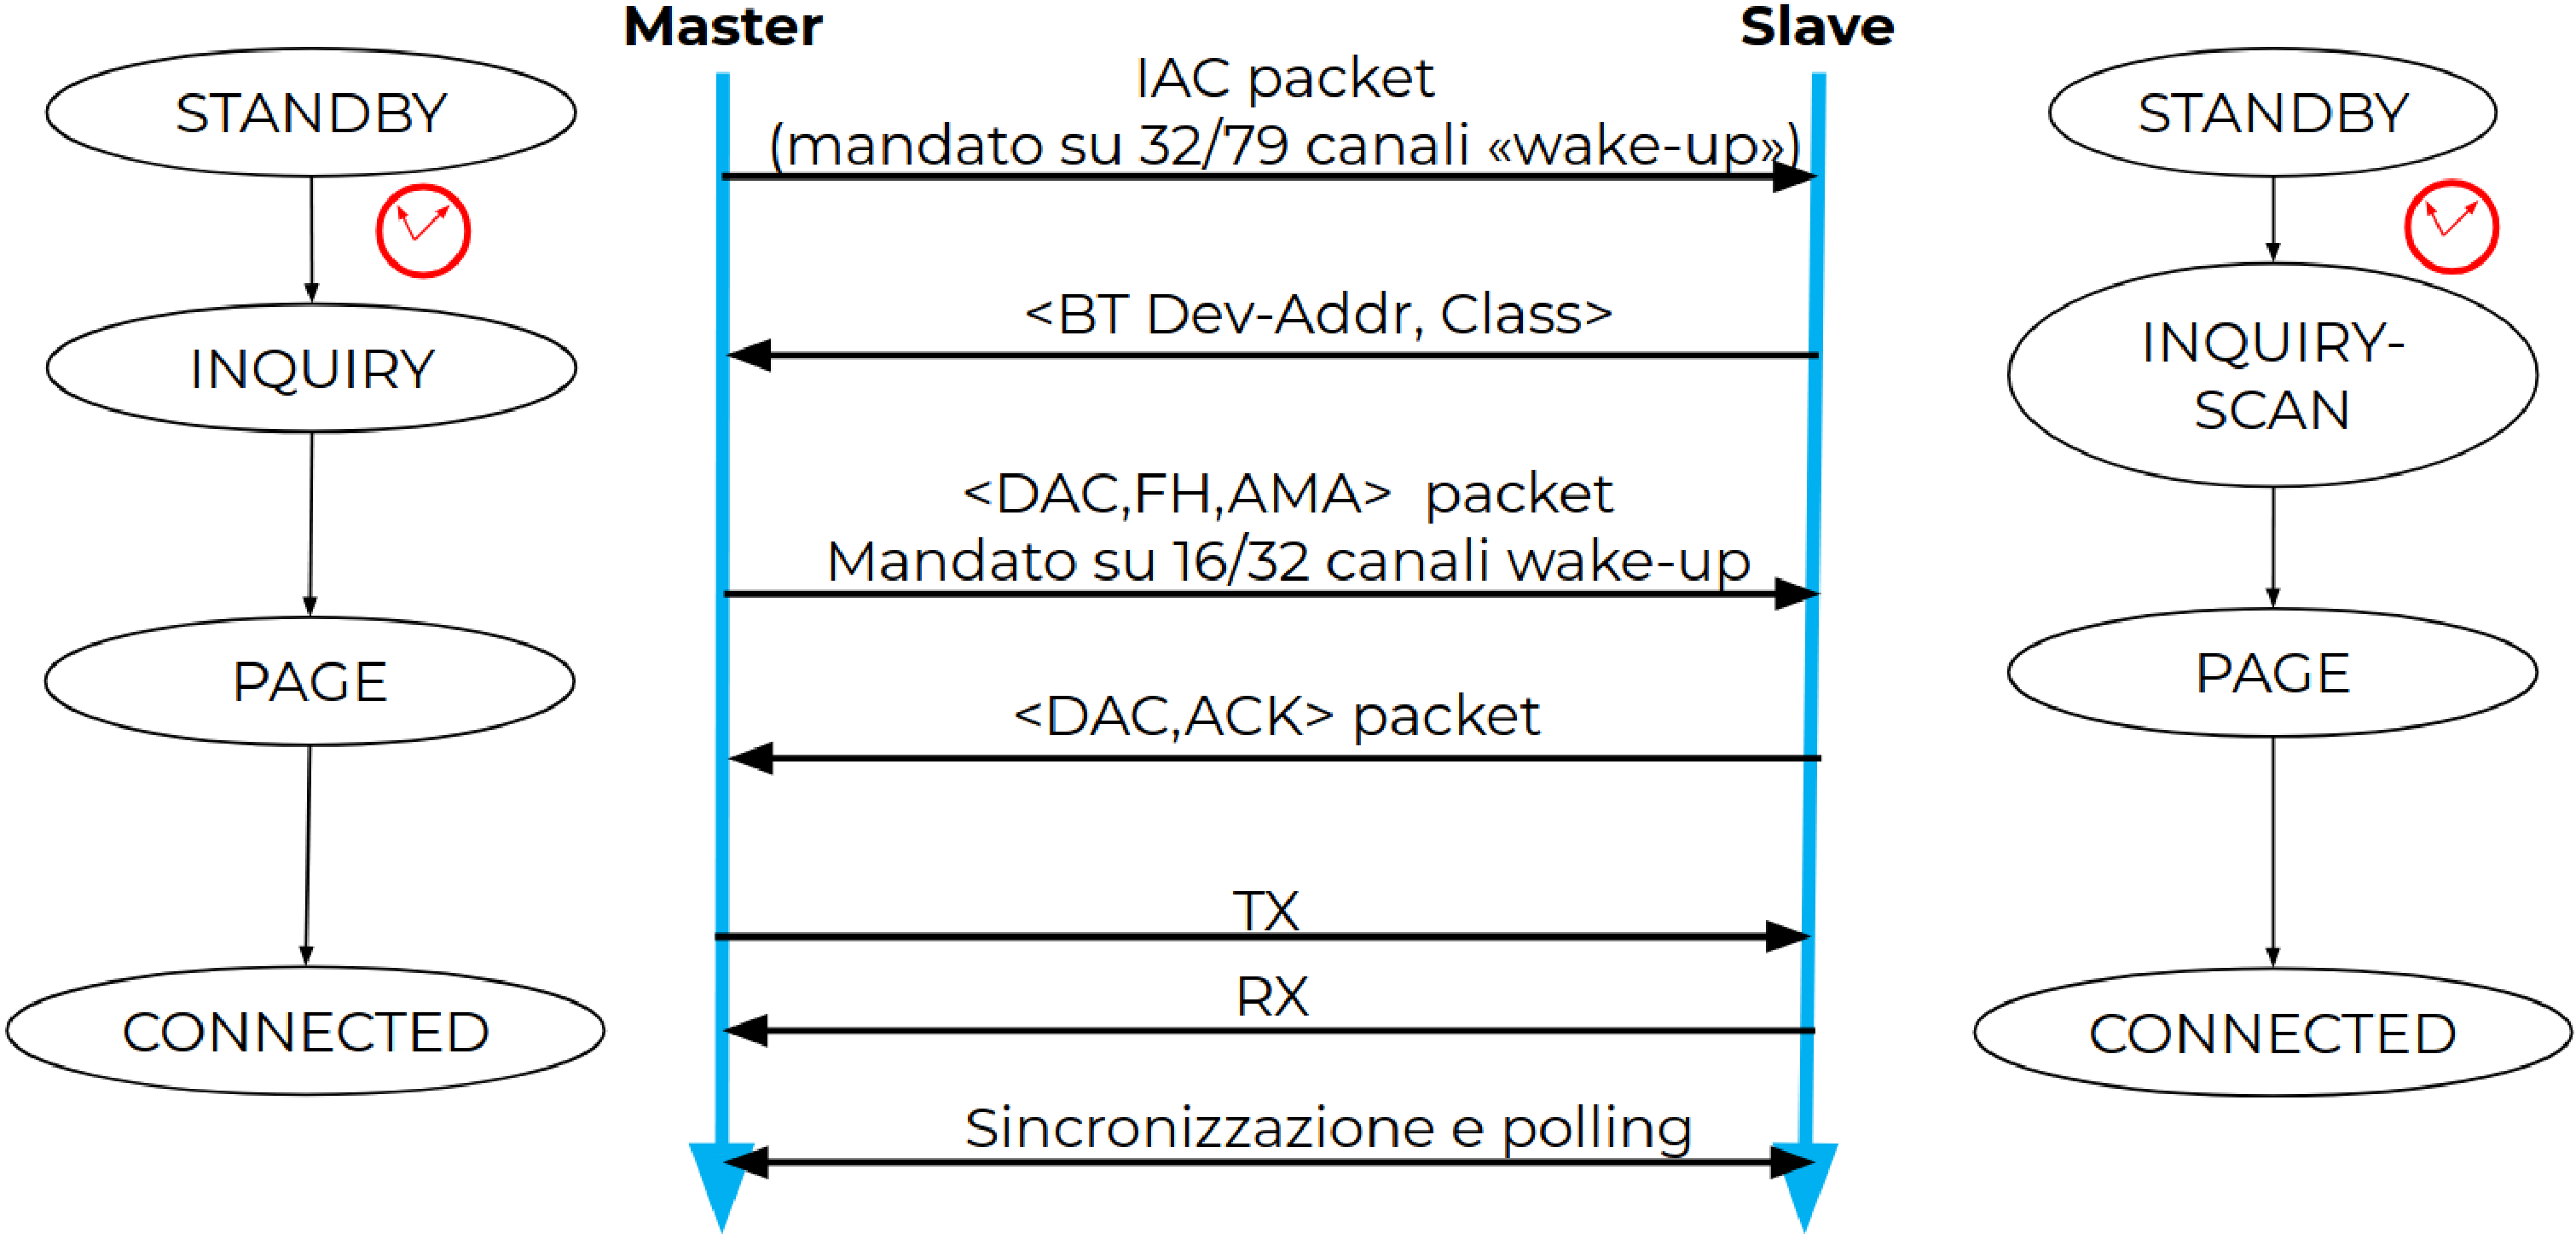
\includegraphics[width=0.95\linewidth]{img/wpan/inquiry1}
\end{center}

%End L6

    % !TeX spellcheck = it_IT
\section{WiFi}

\begin{questions}
    \question Descrivere lo schema di accesso del protocollo 802.11 (Wi-Fi) CSMA/CA. Discutere, inoltre, che "accorgimento" viene aggiunto al meccanismo di backoff per evitare che una stazione attenda un tempo indefinito per accedere al canale.
    
    \begin{solution}
        Il sistema Carrier Sense Multiple Access/Collision Avoidance CSMA/CA richiede di aspettare "del tempo" prima di poter trasmettere. Definizioni delle unità di tempo: 
        \begin{itemize}
            \item Slot time: unità base di tempo, dipende dal trasmettitore fisico usato 
            
            \item SIFS: intervallo più breve, usato per messaggi ad alta priorità
            
            \item DIFS: intervallo più lungo, usato per messaggi a bassa priorità, pari a SIFS+2 slot time
            
            \item PIFS: intervallo di tempo intermedio, usato per servizi time-bounded, SIFS+slot time
        \end{itemize}
        
        Per trasmettere, un dispositivo: 
        \begin{itemize}
            \item Verifica che il canale sia libero tramite un Clear Channel Assessment CCA
            
            \item Ascolta per tempo DIFS il canale 
            
            \item fa un altro CCA 
        \end{itemize}
        Se il canale è risultato libero entrambe le volte, può cominciare a comunicare.
        
        Se il canale è occupato: il dispositivo aspetta il termine dell'altra trasmissione, per poi attendere tempo DIFS più un numero random di slot time (random backoff). Viene fatto carrier sense durante tutto il periodo di backoff, se il canale risulta libero può cominciare a trasmettere.
        
        Se durante il periodo di contesa il canale torna occupato, al turno successivo il dispositivo riprende il conteggio degli slot dal valore a cui era arrivato.
        
        Se necessario ack, il dispositivo attende tempo SIFS per riceverlo al termine della sua trasmissione, prima di presupporre che il frame sia stato corrotto e ritrasmettere.
    \end{solution}
    
    \question Descrivere, con un esempio, il problema del terminale nascosto in una rete Wi-Fi che adotta il protocollo CSMA/CA per l'accesso al canale radio condiviso. Quali modifiche vengono introdotte al protocollo CSMA/CA per risolvere questo problema? 
    
    \begin{solution}
        Se due terminali A e B, fuori dal rispettivo raggio di copertura, volessero trasmettere a B, vedrebbero il canale libero contemporaneamente, in quanto il meccanismo di carrier sense funziona solo se l'altro dispositivo che comincia a trasmettere può essere rilevato.
        
        Per risolvere il problema, il sender, dopo aver fatto carrier sense, invia una Request to Send RTS, contenete origine, destinazione e durata stimata della comunicazione da inviare, in questo modo tutti i terminali che ricevono la RTS senza esserne destinatari possono allocare un Network Allocation Vector NAV per la durata della comunicazione, in cui sanno che il canale verso la destinazione indicata sarà occupato.
        
        Il destinatario del messaggio risponde con un messaggio di Clear to Send CTS, anch'esso contenente origine, destinazione e durata stimata (rimanente) del messaggio. In questo modo anche i terminali all'interno del raggio di copertura del destinatario possono allocare un NAV per la durata della comunicazione.
    \end{solution}
\end{questions}

    % !TeX spellcheck = it_IT

%Controllare anche RFC per studiare
\section{Ad Hoc Distance Vector Routing Protocol AODV}

Ambito WLAN. Si tratta di un \textbf{protocollo di routing}: ha il compito di \textbf{creare e riempire le tabelle di instradamento}. Pensato per una \textbf{rete senza infrastrutture} in cui ogni nodo è anche un router (può fare instradamento). I cammini possono essere multi-hop. I nodi vicini sono quelli nel raggio radio, di conseguenza nodi e vicinati possono variare.\\
I percorsi non vengono creati in modo proattivo: quando serve mandare qualcosa viene richiesto il percorso.\\

Gli \textbf{obiettivi} principali del protocollo sono:
\begin{itemize}
	\item Gestione dinamica della rete ad hoc, ogni nodo può operare secondo protocollo
	\item Auto inizializzante, non sono necessarie rotte preconfigurate; l'inizializzazione deve essere fatta in automatico e periodicamente (per "colpa" della dinamicità della rete)
	\item Loop-free (eliminando il problema del counting to infinity)
	\item Ottenimento di una rotta per una nuova destinazione in tempi rapidi
	\item Risposta rapida alla rottura dei link e al cambio di topologia
\end{itemize}

Le \textbf{funzionalità} che offre sono:
\begin{itemize}
	\item Scoprire e costruire i percorsi per le nuove destinazioni
	\item Mantenere i percorsi in modalità soft-state; ogni percorso ha una durata, se non "rinfrescata" la entry scade e può essere cancellata (eventually)
	\item Riconoscimento errori e cancellazione di percorsi; monitoraggio dell'attività locale e propagazione delle informazioni
\end{itemize}

Si tratta di un protocollo a livello di applicazione (usa UPD 654) che permette di creare tabelle di routing a livello di rete. Ogni nodo è responsabile delle proprie entry, il protocollo è completamente distribuito.\\

\newpage

I dati vengono inviati tra originator e destinazione tramite percorsi simmetrici, non ci sono percorsi indipendenti.
\begin{center}
	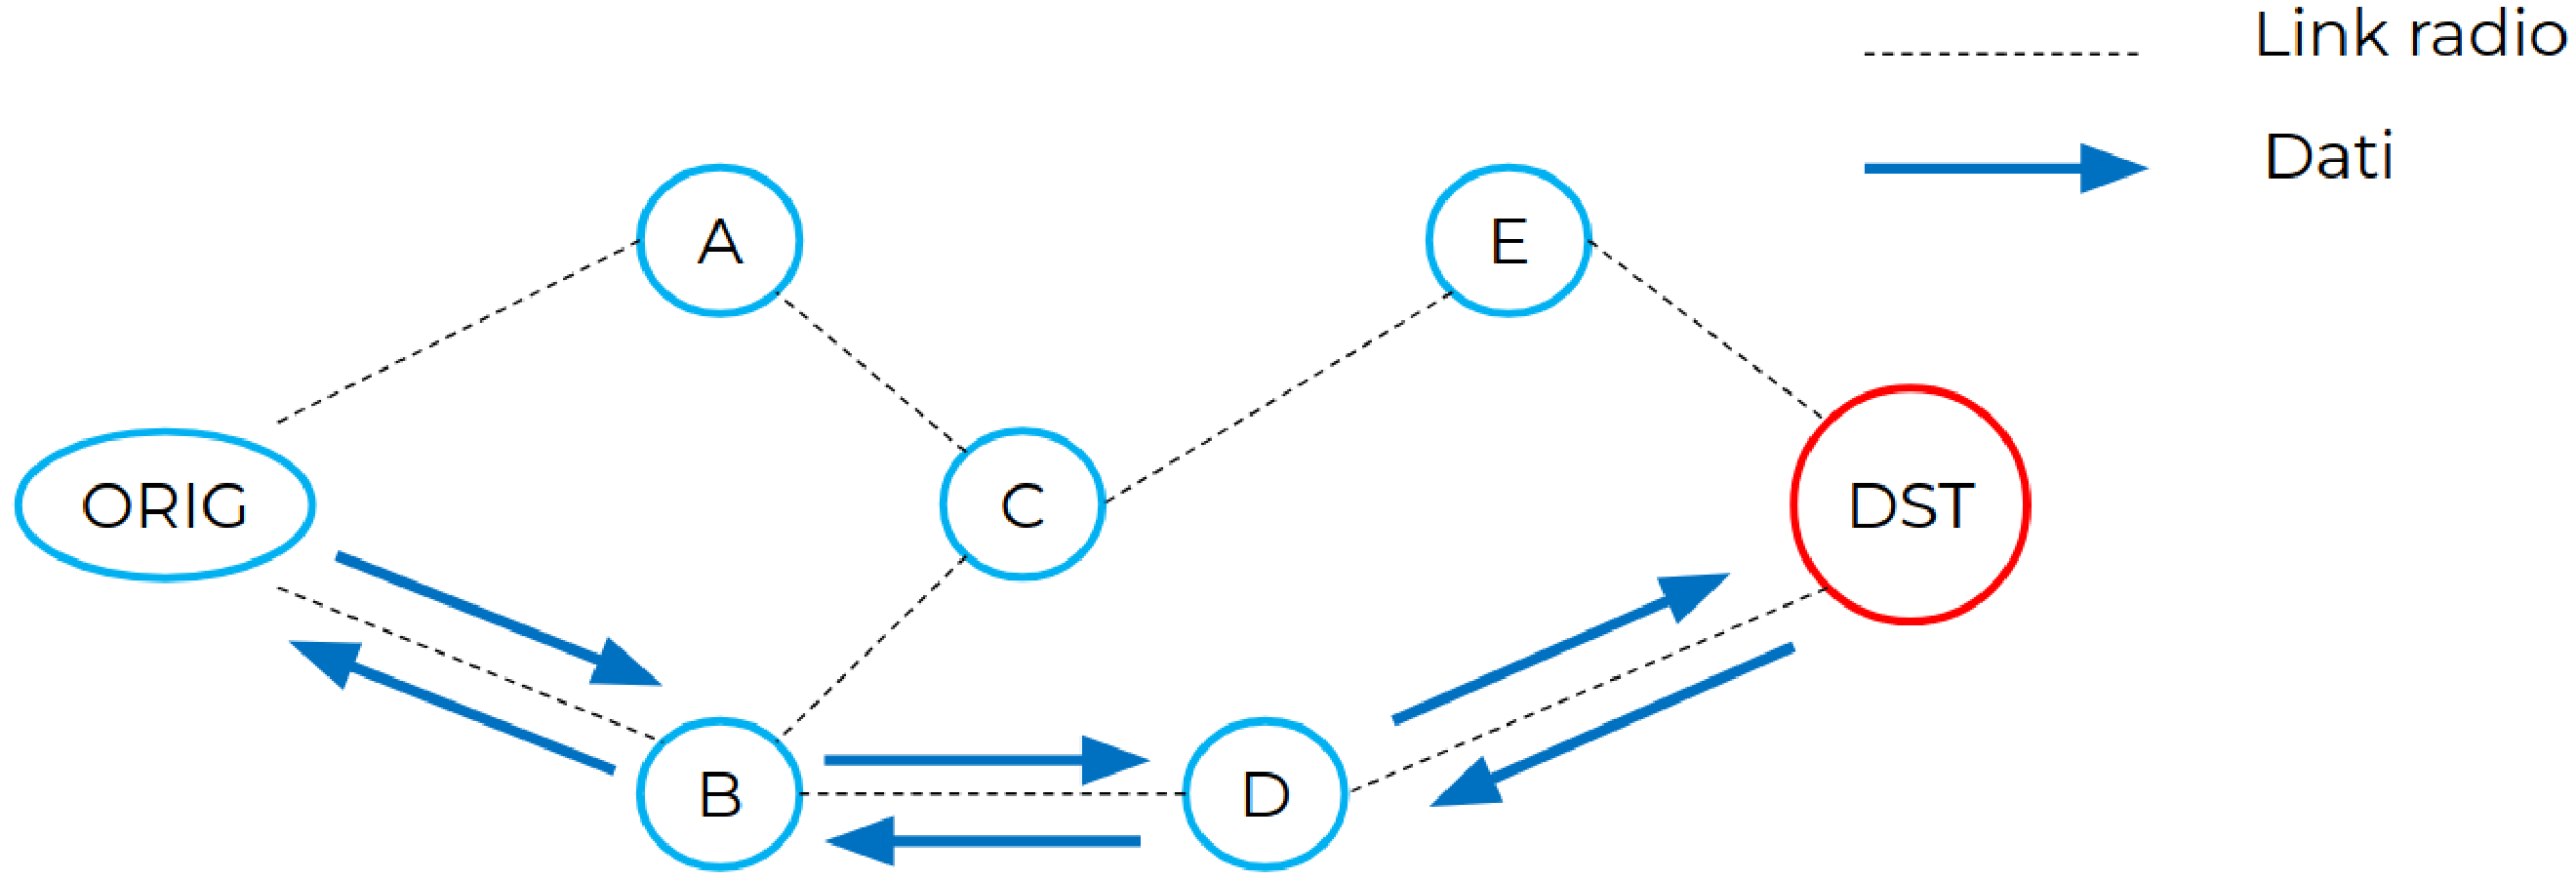
\includegraphics[width=0.9\linewidth]{img/aodv/path1}
\end{center}

\paragraph{Route Request:} I percorsi vengono costruiti tramite \textbf{Route Request RREQ}, sono pacchetti di controllo che permettono di chiedere la costruzione di un percorso verso la destinazione. Non sapendo niente, i messaggi RREQ vengono inviati in broadcast "controllato" (senza loop, il broadcast è fatto a livello IP, con l'indirizzo IP di broadcast). Ogni nodo inoltra RREQ e tiene traccia della provenienza.\\

\paragraph{Route Reply:} La destinazione richiesta in una RREQ risponde in unicast con un messaggio \textbf{Route Reply RREP}.
\begin{center}
	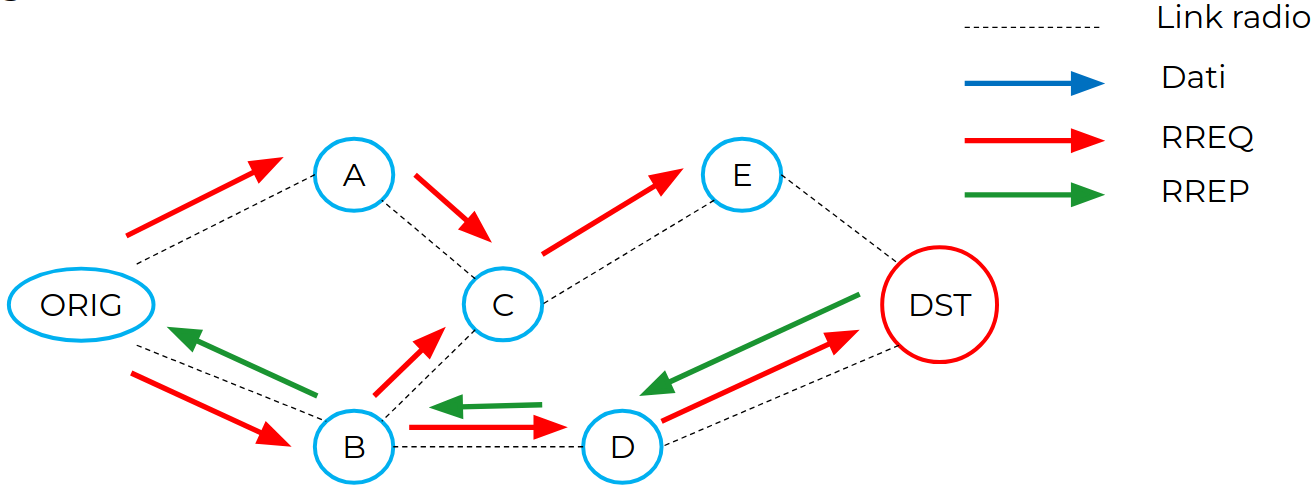
\includegraphics[width=0.9\linewidth]{img/aodv/path2}
\end{center}

La destinazione manda la risposta RREP solo alla prima RREQ (con lo stesso identificatore) ricevuta, in modo da evitare risposte duplicate e trovando (circa) il percorso più breve, dato che risponderà solo al messaggio che ci ha impiegato meno tempo (il primo arrivato).\\

Anche un nodo intermedio può fornire la risposta (inviare il RREP), se conosce l'informazione (sa come arrivare a destinazione) ed è abbastanza "fresca" (lo ha saputo di recente).\\

\paragraph{Route Error:} Un altro messaggio di controllo è \textbf{Route Error RERR}, usato nel caso un link si rompe, per qualsiasi motivo. Il nodo lo invia a tutti i vicini che sa utilizzano quel link per arrivare ad una qualche destinazione.\\

Lo stack è:

\begin{center}
	\renewcommand{\arraystretch}{1.4}
	\begin{tabular}{>{\centering\arraybackslash}m{4cm} | >{\centering\arraybackslash}m{3.5cm} | >{\centering\arraybackslash}m{3.5cm} |}
		\cline{2-3}
		& Messaggi Dati & RREQ/RREP/RERR \\
		\hline
		Livello applicazione & Protocollo\newline applicazione & AODV \\
		\hline
		Livello Trasporto & Trasporto \newline UPD/TCP/\dots & UPD Porta 654 \\
		\hline 
		Livello Rete & \multicolumn{2}{c |}{IP} \\
		\hline
		Livello data link (LL) & \multicolumn{2}{c |}{Ethernet (802.3)/WiFi(802.11)/802.15.4/\dots} \\
		\hline
		Livello fisico (PHY) & \multicolumn{2}{c |}{Ethernet (802.3)/WiFi(802.11)/802.15.4/\dots} \\
		\hline
	\end{tabular}
\end{center}
Quindi i messaggi possono essere dati "normali" tramite TCP oppure i messaggi di controllo AODV. Il livello di rete è IP, mentre i livelli di data link e fisico possono essere uno qualsiasi degli standard IEEE previsti.\\

\subsection{Tabelle di Routing}

Ogni nodo mantiene una tabella delle destinazioni conosciute e l'indicazione del prossimo hop lungo il percorso. Ogni entry in una tabella contiene:
\begin{itemize}
	\item IP destinazione
	\item Sequence number della destinazione
	\item Flag di validità del sequence number della destinazione; permette di disabilitare/abilitare temporaneamente un percorso
	\item Stato del percorso (valido, invalido e altri)
	\item Interfaccia di rete
	\item Hop count, numero di hop per arrivare alla destinazione, ovvero il costo
	\item Lista dei precursori, quali sono i vicini che utilizzano "me" (il nodo) per arrivare a destinazione
	\item Lifetime della entry, ovvero il tempo di scadenza
\end{itemize}

\paragraph{Sequence Number SN:} Tutto cambia in questa rete, quindi ogni entry della tabella possiede un SN che codifica informazioni circa "\textit{la freschezza}" della entry stessa. Il SN è un valore per ogni nodo, ogni possibile destinazione (nodo) ha il proprio e viene modificato esclusivamente dal nodo stesso. \\

Il SN viene incrementato dal nodo in 2 casi: 
\begin{enumerate}
	\item Quando un nodo inizia una ricerca di percorso (RREQ), viene incrementato di 1, previene conflitti con i percorsi inversi stabiliti da una precedente RREQ
	\item Quando un nodo risponde (ovvero il nodo è la destinazione) ad una richiesta di percorso (manda RREP); si aumenta di 1 (solo in alcuni casi in realtà)
\end{enumerate}

Gli altri nodi possono aggiornare il sequence number di una entry in tabella se: 
\begin{itemize}
	\item Il nodo stesso offre un nuovo percorso per se stesso (aggiorna la propria entry nella sua tabella di routing)
	\item Il nodo riceve informazioni più aggiornate per un destinazione
	\item Il percorso verso quella destinazione è scaduto/interrotto
\end{itemize}

Il SN viene confrontato per capire \textit{chi ha l'informazione più aggiornata} per la destinazione. L'incremento viene fatto come se fosse unsigned, il confronto come signed (per gestire overflow).\\

\newpage

\subsection{RREQ}

\paragraph{Formato:} Il formato di una RREQ è 
\begin{verbatim}
	 0                   1                   2                   1
	 0 1 2 3 4 5 6 7 8 9 0 1 2 3 4 5 6 7 8 9 0 1 2 3 4 5 6 7 8 9 0 1
	+-+-+-+-+-+-+-+-+-+-+-+-+-+-+-+-+-+-+-+-+-+-+-+-+-+-+-+-+-+-+-+-+
	|     Type      |J|R|G|D|U|   Reserved          |   Hop Count   |
	+-+-+-+-+-+-+-+-+-+-+-+-+-+-+-+-+-+-+-+-+-+-+-+-+-+-+-+-+-+-+-+-+
	|                            RREQ ID                            |
	+-+-+-+-+-+-+-+-+-+-+-+-+-+-+-+-+-+-+-+-+-+-+-+-+-+-+-+-+-+-+-+-+
	|                    Destination IP Address                     |
	+-+-+-+-+-+-+-+-+-+-+-+-+-+-+-+-+-+-+-+-+-+-+-+-+-+-+-+-+-+-+-+-+
	|                  Destination Sequence Number                  |
	+-+-+-+-+-+-+-+-+-+-+-+-+-+-+-+-+-+-+-+-+-+-+-+-+-+-+-+-+-+-+-+-+
	|                     Originator IP Address                     |
	+-+-+-+-+-+-+-+-+-+-+-+-+-+-+-+-+-+-+-+-+-+-+-+-+-+-+-+-+-+-+-+-+
	|                  Originator Sequence Number                   |
	+-+-+-+-+-+-+-+-+-+-+-+-+-+-+-+-+-+-+-+-+-+-+-+-+-+-+-+-+-+-+-+-+
\end{verbatim}

Il \textbf{tipo} è 1, rappresenta il tipo di pacchetto di controllo inviato (RREQ in questo caso).\\

Le \textbf{flag} sono: 
\begin{itemize}
	\item \textbf{\texttt{D}}: Destination Only, solo la destinazione può rispondere, niente nodi intermedi
	\item \textbf{\texttt{U}}: Unknown SN, l'origine non conosce SN della destinazione
	\item \textbf{\texttt{G}}: (Gratuitous) RREP, un nodo intermedio, oltre a rispondere all'origine, deve informare la destinazione della creazione di un percorso (reverse) con l'origine
\end{itemize}

L'\textbf{hop count} viene incrementato di 1 ogni volta che viene inoltrata la RREQ, serve a tenere traccia del "costo" del percorso, in realtà la destinazione vuole rispondere alla RREQ con hop count minore.\\

Il \textbf{RREQ ID} è l'identificativo della richiesta, generato dall'origine e mai modificato, serve a riconoscere la richiesta e le sue copie come un'unica richiesta all'interno della rete.\\

\newpage

Il \textbf{Destination IP Address} è l'indirizzo della destinazione ed il SN indicato è l'ultimo conosciuto (o nessuno nel caso il flag \texttt{U} sia alzato). Se un nodo intermedio ha informazioni riguardo alla destinazione, ma con SN inferiore rispetto a quello indicato, sicuramente l'informazione è troppo vecchia quindi non la invia.\\

\textbf{Originator IP Address} e \textbf{SN} sono le informazioni riguardo l'originator, con il SN più recente inviato.\\

\paragraph{RREQ Creation:} Una RREQ viene creata \textit{quando serve}, ovvero quando un nodo non conosce la destinazione o se la entry è scaduta. Per inviare:
\begin{itemize}
	\item Incremento RREQ ID e il proprio SN (dell'originator)
	\item Se la destinazione è sconosciuta, flag \texttt{U}$=1$
	\item Mantiene una copia di Origine IP, RREQ ID per un tempo denominato \texttt{PATH\_DISCOVERY\_TIME}, definito nello standard, per evitare il riprocessamento e il reinvio dei pacchetto che può essere ricevuto dai vicini
\end{itemize}

\subsubsection{Expanding Ring Search}
 Vogliamo evitare di propagare "inutilmente" una RREQ in tutta la rete, magari la destinazione è vicina. Il TTL dell'header IP viene usato per impostare il massimo numero di hop che una RREQ può fare.\\

Si hanno dei parametri:
\begin{itemize}
	\item \textbf{\texttt{TTL\_START}}: parametro TTL per la prima richiesta
	\item \textbf{\texttt{TTL\_INCREMENT}}: incremento del TTL ad ogni tentativo
	\item \texttt{\textbf{NET\_DIAMETER}}: massimo valore del TTL
\end{itemize}

La request viene fatta inizialmente con un TTL basso, se dopo una certa quantità di tempo il nodo non riceve risposta viene aumentato il TTL ed effettuata una nuova richiesta ("bah, magari è più lontana, ci riprovo"). Ripete fino al TTL massimo. Si espande "l'anello" in cui cercare la destinazione.\\

Questo era \textit{senza conoscenze a priori}, se sono presenti delle conoscenze riguardo un percorso verso la destinazione (scaduto o interrotto) uso la distanza nota in precedenza per iniziare a inviare RREQ. Se ho un'informazione vecchia: parto dalla distanza "vecchia" come TTL. Questo è uno dei motivi per cui non "buttare" subito le informazioni vecchie, vengono tenute per "\textit{un po'}" (definito dallo standard).\\

\paragraph{Retry Policy:} L'origine può riprovare ad inviare RREQ se il primo tentativo non è andato a buon fine. \texttt{\textbf{RREQ\_RETRIES}} è il parametro. Ad ogni nuovo tentativo si incrementano RREQ\_ID e SN.\\

\subsubsection{RREQ Processamento e Inoltro}

Quando un nodo riceve un messaggio RREQ:
\begin{itemize}
	\item Controlla REQ\_ID e Originator IP sono già presenti (già conosciute), se uguali all'ultimo ricevuto entro \texttt{PATH\_DISCOVERY\_TIME} scarto il messaggio
	\item Aggiorno il percorso "reverse", verso originator; ricevendo una RREQ posso capire come arrivare all'origine:
	\begin{enumerate}
		\item Confronto Orig SN (in RREQ) e SN che ho nella tabella, se è maggiore lo aggiorno (potrebbe essere minore, magari la richiesta è molto vecchia, ha fatto giri strani)
		\item Segno la entry come valida (può essere scaduta nel frattempo)
		\item Aggiorno/aggiungo la entry impostando come "next hop" verso orig, il nodo da cui è arrivata la RREQ
		\item Il campo Hop Count della entry viene messo pari al hop count della RREQ (quanto ci ha messo ad arrivare al nodo)
	\end{enumerate}
\end{itemize}

%End L13

Se il nodo intermedio non può rispondere con RREP (anche per flag \texttt{D}) allora deve inoltrare RREQ ai vicini. Per farlo, modifica il messaggio RREQ:
\begin{itemize}
	\item incrementa di 1 Hop Count
	\item il SN della DST (in RREQ) deve essere il massimo tra quello nella richiesta e il SN nella routing table (la richiesta è "vecchia", ho informazioni più nuove)
	\item manda la RREQ in broadcast (indirizzo IP 255.255.255.255)
\end{itemize}
In questo modo, il propagarsi di una richiesta permette ai nodi che la ricevono di costruire un percorso verso l'orig.\\

\subsection{RREP}

\paragraph{Formato:} 
\begin{verbatim}
	0                   1                   2                   1
	0 1 2 3 4 5 6 7 8 9 0 1 2 3 4 5 6 7 8 9 0 1 2 3 4 5 6 7 8 9 0 1
	+-+-+-+-+-+-+-+-+-+-+-+-+-+-+-+-+-+-+-+-+-+-+-+-+-+-+-+-+-+-+-+-+
	|     Type      |R|A|    Reserved     |Prefix sz|   Hop Count   |
	+-+-+-+-+-+-+-+-+-+-+-+-+-+-+-+-+-+-+-+-+-+-+-+-+-+-+-+-+-+-+-+-+
	|                     Destination IP Address                    |
	+-+-+-+-+-+-+-+-+-+-+-+-+-+-+-+-+-+-+-+-+-+-+-+-+-+-+-+-+-+-+-+-+
	|                  Destination Sequence Number                  |
	+-+-+-+-+-+-+-+-+-+-+-+-+-+-+-+-+-+-+-+-+-+-+-+-+-+-+-+-+-+-+-+-+
	|                     Originator IP Address                     |
	+-+-+-+-+-+-+-+-+-+-+-+-+-+-+-+-+-+-+-+-+-+-+-+-+-+-+-+-+-+-+-+-+
	|                           Lifetime                            |
	+-+-+-+-+-+-+-+-+-+-+-+-+-+-+-+-+-+-+-+-+-+-+-+-+-+-+-+-+-+-+-+-+
\end{verbatim}

Qua il tipo è 2.\\

Flag:
\begin{itemize}
	\item \texttt{A}: acknowledgment richiesto in risposta per prevenire link non affidabili
\end{itemize} 

Il \textbf{prefix size} viene utilizzato per subnet, indica la lunghezza del prefisso di rete dell'indirizzo IP di destinazione (in bit).\\

Il \textbf{destination IP Address} indica chi ha generato la risposta.\\

Il \textbf{destination Sequence Number} si riferisce al SN più aggiornato della destinazione.\\

L'\textbf{originator IP Address} indica a chi sta rispondendo questa richiesta.\\

\textbf{Lifetime}: determinato da chi crea RREP, millisencondi di validità della risposta.\\

\paragraph{Creazione:} Chi può generare una RREP?
\begin{enumerate}
	\item La \textbf{destinazione}
	\begin{itemize}
		\item Incrementa il suo SN prima di inviare
		\item Hop count $= 0$
		\item Aggiorna la lista dei precursori (chi usa la destinazione stessa come hop)
		\item Imposta il campo lifetime \texttt{MY-ROUTE-TIMEOUT} (default 6s)
		\item Invia RREP lungo il percorso reverse (unicast)
		\item Effettua il drop della RREQ (non viene più inoltrata)
	\end{itemize}
	
	\item Un \textbf{nodo intermedio}: può farlo, ma con delle condizioni:
	\begin{enumerate}
		\item Avere una entry con un percorso valido per la destinazione
		\item Flag \texttt{D == 0}
		\item DST SN della entry $\geq$ DST SN della RREQ
	\end{enumerate}
	Se tutte soddisfatte, allora:
	\begin{itemize}
		\item Hop count = valore Hop count della entry (distanza dalla destinazione, al posto dello 0 di prima)
		\item Aggiorna la lista dei precursori (il nodo a cui sto inviando la RREP userà "me" come hop per arrivare alla destinazione)
		\item Imposta il campo lifetime in base a quello che ho nella entry (il tempo che rimane nella entry)
		\item Invio RREP lungo il percorso reverse in unicast
		\item Drop della RREQ
		\item Se il flag \texttt{G == 1} allora invio RREP anche alla destinazione (vedi dopo)
	\end{itemize}
\end{enumerate}

\subsubsection{RREP Processamento e Inoltro}

Quando un nodo riceve un messaggio RREP:
\begin{itemize}
	\item Aggiorna la entry nella tabella se
	\begin{itemize}
		\item La entry corrente non è valida
		\item DST SN della RREP è maggiore di quello della entry
		\item Il numero di hop è minore rispetto a quello della entry
	\end{itemize}

	\item Aggiorna
	\begin{itemize}
		\item Entry marcata come valida
		\item Next hop della entry $=$ nodo da cui proviene RREP (destinazione della RREQ)
		\item Aggiorno RREP hop count, incremento di 1
		\item Aggiorno campo lifetime della entry
		\item Aggiorno la lista dei precursori (chi sta usando "me" per raggiungere l'originator)
	\end{itemize}
\end{itemize}

Mentre torna la RREP, ogni nodo intermedio crea il path da se stesso alla destinazione originale della RREQ. Ma il percorso "bidirezionale" viene creato solo nella porzione di rete tra il nodo intermedio e l'originator, non anche verso la destinazione.\\
%Si risolve con G?

Dopo la RREP di un nodo intermedio, dato che la RREQ originale era in broadcast, anche la sorgente (eventually) invierà la sua RREP. Entrambe le RREP torneranno all'originator, probabilmente quella della destinazione arriverà dopo, in qualsiasi caso la migliore viene tenuta (SN maggiore e Hop count minore).\\

\paragraph{RREP a RREQ con flag Gratuitous:} Se un nodo intermedio riceve una RREQ con flag gratuitous attivo, il nodo deve occuparsi di "costruire" il rimanente percorso verso la destinazione della RREQ.\\

Il nodo quindi invia 2 RREP indipendenti
\begin{enumerate}
	\item Verso il nodo Origine (che ha creato la RREQ)
	\item Verso la destinazione della RREQ (Gratuitous), con 
	\begin{itemize}[noitemsep]
		\item Hop count = numero hop nella entry verso origine RREQ
		\item Destinazione = IP origine delle RREQ
		\item Destinazione SN = SN nella entry verso origine RREQ
		\item Originator IP = DST della RREQ
		\item Lifetime = lifetime nella entry verso origine RREQ
	\end{itemize}
\end{enumerate}

Serve a "simulare" che la destinazione abbia fatto una reply, finisco di costruire il percorso tra nodo intermedio e destinazione. Mi garantisce che il nodo di destinazione e tutti quelli sul percorso conoscano la strada per arrivare anche all'originator della RREQ iniziale. Come se il nodo destinazione avesse fatto una RREQ verso l'originator (i parametri della RREP sono quelli), completando il path bidirezionale.\\

\subsubsection{Hello Message}

Ogni nodo può indicare informazioni riguardo la propria connettività inviando periodicamente in broadcast degli "hello message" ai propri vicini. Si tratta di un messaggio broadcast con \texttt{TTL = 1} (senza incrementare il SN, lascio quello più recente). \\

Si tratta di una RREP speciale, con i seguenti campi: 
\begin{itemize}
	\item DST IP = IP del nodo stesso
	\item DST SN = SN del nodo stesso
	\item Hop Count = 0
	\item Lifetime = \texttt{ALLOWED\_HELLO\_LOSS} * \texttt{HELLO\_INTERVAL}
\end{itemize}

Si tratta di un meccanismo facoltativo e sono usati solo se non si ricevono altri pacchetti da un vicino, qualunque pacchetto valido può essere usato per aggiornare la "vicinanza" di un nodo.\\

\newpage

\subsection{Mantenimento della Connettività Locale}

Ogni nodo ha come compito tenere traccia della connettività con i nodi indicati come "next hop" nelle entry della tabella di routing.\\

Ci sono diversi meccanismi:
\begin{enumerate}
	\item \textbf{Livello data-link}: invio pacchetto RTS/CTS/ACK, in caso di mancanza di CTS/ACK \textit{probabilmente} il link non è più valido
	\item \textbf{Livello di rete}: la ricezione di qualsiasi pacchetto dal next hop è \textit{un'informazione} (quindi il link è attivo e posso mantenere entry), ad esempio una RREQ con destinazione il next hop, ICMP Echo unicast per il next hop (ping)
\end{enumerate}

\paragraph{Percorso interrotto/scaduto e cancellazione:} Quando un nodo identifica un link interrotto il quale è parte di un percorso attivo:
\begin{enumerate}
	\item Vengono invalidati i percorsi esistenti
	\item Identifica le destinazioni per le quali viene usato come next hop il link interrotto
	\item Determina quali vicini possono essere affetti da questo problema (lista dei predecessori)
	\item A questi vicini invia un messaggio di \textbf{Route Error RERR}
\end{enumerate} 

\paragraph{Formato RERR:}
\begin{verbatim}
	0                   1                   2                   1
	0 1 2 3 4 5 6 7 8 9 0 1 2 3 4 5 6 7 8 9 0 1 2 3 4 5 6 7 8 9 0 1
	+-+-+-+-+-+-+-+-+-+-+-+-+-+-+-+-+-+-+-+-+-+-+-+-+-+-+-+-+-+-+-+-+
	|     Type      |R|A|    Reserved     |Prefix sz|   Hop Count   |
	+-+-+-+-+-+-+-+-+-+-+-+-+-+-+-+-+-+-+-+-+-+-+-+-+-+-+-+-+-+-+-+-+
	|            Unreachable Destination IP Address (1)             |
	+-+-+-+-+-+-+-+-+-+-+-+-+-+-+-+-+-+-+-+-+-+-+-+-+-+-+-+-+-+-+-+-+
	|        Unreachable Destination Sequence Number (1)            |
	+-+-+-+-+-+-+-+-+-+-+-+-+-+-+-+-+-+-+-+-+-+-+-+-+-+-+-+-+-+-+-+-+
	|  Additional Unreachable Destination IP Addresses (if needed)  |
	+-+-+-+-+-+-+-+-+-+-+-+-+-+-+-+-+-+-+-+-+-+-+-+-+-+-+-+-+-+-+-+-+
	|Additional Unreachable Destination Sequence Numbers (if needed)|
	+-+-+-+-+-+-+-+-+-+-+-+-+-+-+-+-+-+-+-+-+-+-+-+-+-+-+-+-+-+-+-+-+
\end{verbatim}

Il tipo è 3. 

L'unica \textbf{flag} \texttt{N} indica alla destinazione della RERR di non eliminare la entry (No Delete flag) perché il percorso è stato riparato localmente. Il nodo che invia con il flag \texttt{N} alzato si è reso conto che il link era rotto, ma lo ha anche riparato (non sullo stesso link, altra RREQ, non importa come), quindi chi riceve il RERR sa che c'è una soluzione e potrebbe mantenere il link, anche se potrebbe essere più lungo o simili. Insomma, si era rotto ma ci ha pensato il nodo.\\

Il \textbf{Dest Count} indica il numero delle destinazioni che non sono più raggiungibili contenute in questo messaggio (quanti link si sono rotti); il numero di coppie a 32 bit all'interno del messaggio.\\

%End L14
    
    % !TeX spellcheck = it_IT
\section{Mobile Network}

L'idea è molteplici trasmettitori, area divisa in celle, ogni cella servita da una Base Station BS, la quale contiene trasmettitore, ricevitore e unità di controllo.

Le celle devono coprire "bene" l'area e avere una disposizione uniforme (comunque considerando vincoli dovuti alla situazione reale).

\paragraph{Riuso delle frequenze:} Celle vicine non possono usare la stessa banda di frequenza. Tre soluzioni possibili: 
\begin{itemize}
    \item \textbf{Frequenze diverse tra celle vicine}: ogni cella ha la sua banda, servono più bande differenti (costano); usato da 2G
    
    \item Usare la \textbf{stessa frequenza ma tecniche di codifica} per evitare interferenze, come CDMA
    
    \item Usare \textbf{frequenze diverse ai bordi} delle celle, l'\textbf{intero spettro al centro}; permette banda maggiore ma richiede coordinamento tra le BS (da 4g e 5G)
\end{itemize}

\paragraph{Architettura:} Si divide in due macro aree: 
\begin{itemize}
    \item \textbf{Radio Access Network RAN:} stazioni e collegamento radio che forniscono connettività ai dispositivi mobili (parte wireless)
    
    \item \textbf{Core Network:} parte responsabile di gestione e controllo della comunicazione
\end{itemize}

In generale, esistono 2 tipologie di canali e traffico:
\begin{itemize}
    \item Canali di controllo: informazioni per la gestione delle operazioni; Control Plane
    
    \item Canali di traffico: voce e dati; Data Plane
\end{itemize}
La divisione tra i due piani è netta ed esplicita.

\subsection{Operazioni}

\paragraph{Inizializzazione:} Quando un dispositivo vuole iniziare una comunicazione con la rete cellulare: 
\begin{itemize}
    \item Disponibilità dei canali radio con BS: ascolta le trasmissioni broadcast delle BS per individuare la migliore e quali parametri usare
    
    \item Traffico di controllo per iniziare la comunicazione: viene inoltrata la richiesta di comunicazione fino al MTSO, parte della CN che si occupa di autenticare l'utente, verificare permesse e risorse
    
    \item Creazione dei collegamenti su data plane: se la fase di controllo va a buon fne, vengono allocati canali fisici e logici necessari per il traffico dati
\end{itemize}

\paragraph{Paging:} Quando \textit{qualcosa} deve raggiungere il dispositivo, è compito della rete trovarne la posizione quando necessario. MTSO contatta le BS per trovare il dispositivo.

\paragraph{Chiamata accettata:} I dati passano sempre per il CN, il dispositivo accetta la chiamata, MTSO crea un circuito e le BS impostano i canali radio data plane. 

\paragraph{Handoff:} Quando un dispositivo esce da una cella, deve collegarsi a un'altra. Le fasi per il cambio cella sono: decidere la nuova associazione, gestirla, riconfigurare i percorsi di comunicazione. 

Il tutto deve avvenire in maniera automatica e trasparente al dispositivo.

La procedure può essere decisa in due modi:
\begin{enumerate}
    \item solo dalla rete: in base al segnale in uplik
    
    \item coinvolgendo il dispositivo: anche in base a feedback sul downlink
\end{enumerate}

Vengono usate diverse metriche, ma il parametro principale è la potenza del segnale ricevuto. Possibili metodi per stabilire quando cambiare BS a cui il dispositivo è collegato: 
\begin{itemize}
    \item \textbf{Solo potenza relativa:} l'associazione viene fatta alla BS con il migliore segnale. Potrebbe portare a cambio continuo tra BS quando sui bordi delle celle e l'handover è costoso
    
    \item \textbf{Soglia di segnale:} L'handover viene fatto nel caso incui il segnale è peggiore di un'altra BS e allo stesso tempo sotto una certa soglia. Come si definiscono le soglie? (difficile)
    
    \item \textbf{Isteresi:} Per far partire l'handover deve esserci una differenza significativa di potenza, risolvendo il ping pong
\end{itemize}

La soluzione reale è combinare i metodi.

L'handover può essere:
\begin{itemize}
    \item \textbf{Hard}: dispositivo associato a una sola BS alla volta, cambio immediato di frequenza
    
    \item \textbf{Soft}: il dispositivo mantiene connettività con entrambe le BS e ne rilascia una quando il segnale è chiaramente dominante; occupa più risorse
\end{itemize}

\paragraph{Duplex:} Può essere gestito come: 
\begin{itemize}
    \item FDD: divisione in frequenza, minore delay, maggiori risorse richieste
    
    \item TDD: una sola frequenza e slot di tempo; maggiore ritardo dovuto all'attesa
\end{itemize}
    
    % !TeX spellcheck = it_IT
\section{Long Term Evolution 4G LTE}

Confronto tra architettura 3G e 4G:
\begin{center}
	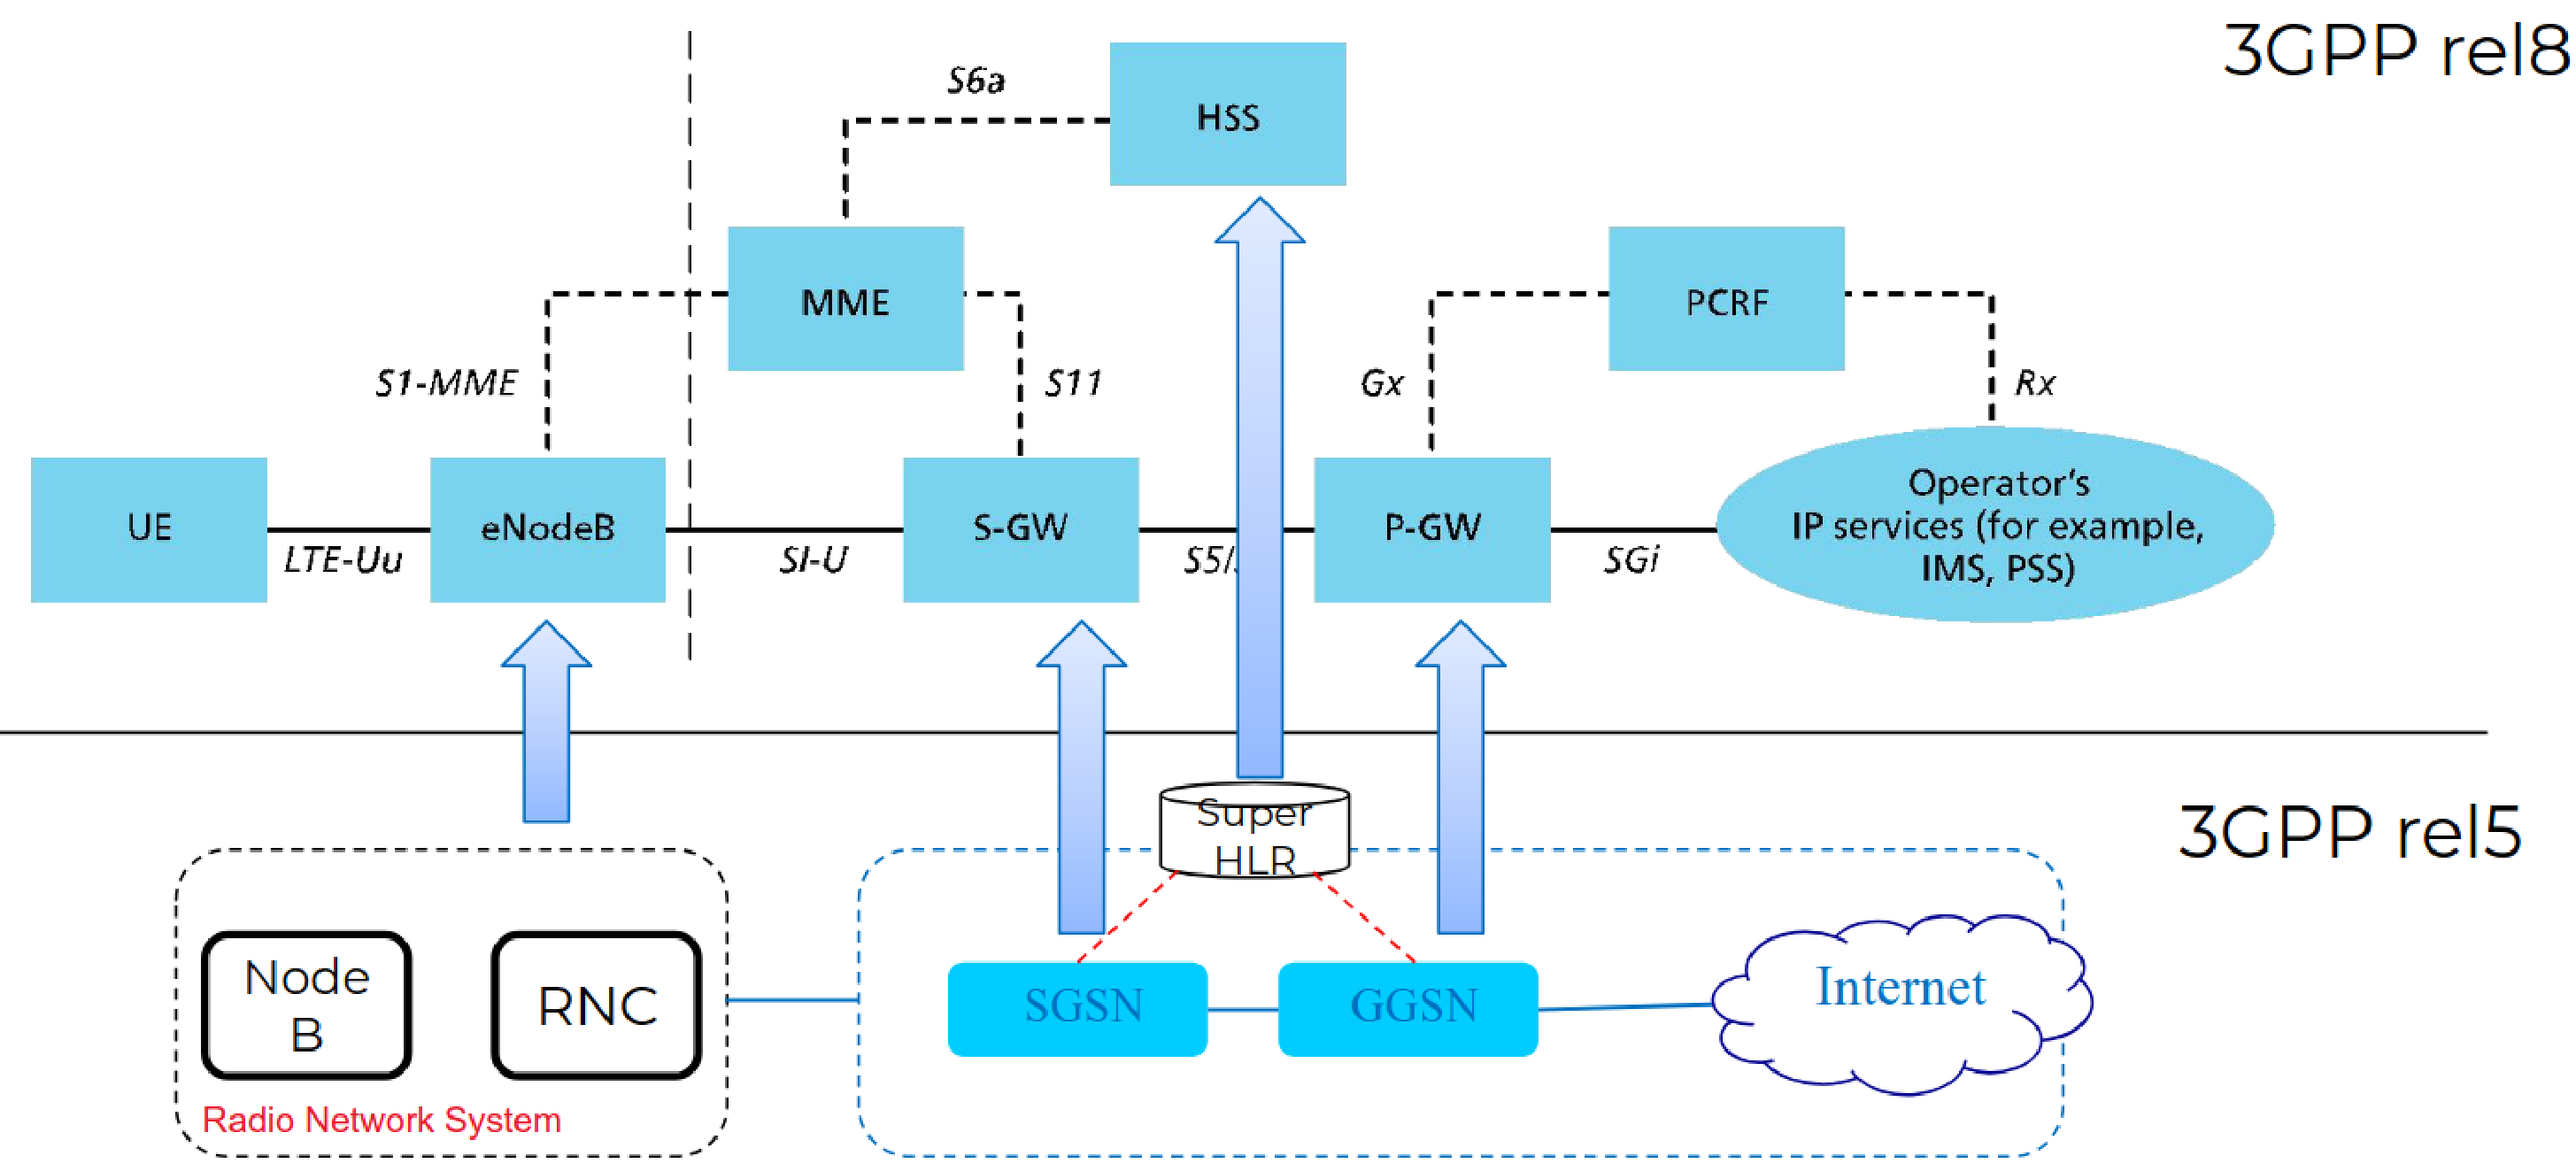
\includegraphics[width=0.98\linewidth]{img/4g/3g4g}
\end{center}

Alcune differenze: 
\begin{center}
	\begin{tabular}{| m{3.5cm} | m{2cm} | m{2cm} |}
		\hline
		& 3G & 4G \\
		\hline
		Separazione logica di Control e Data plane &  No & Sì \\
		\hline
		Accesso multiplo  &WCDMA & OFDMA \\
		\hline
		Riuso frequenze & 100\% & 100\% flessibile \\
		\hline
		Larghezza banda & $5 MHz$ & $1.4$, $3$, $5$, $10$, $15$, $20 MHz$ \\
		\hline		
		Componenti rete accesso & NodeB e RNC & eNodeB \\
		\hline
		Handover & Soft e Hard & Hard \\
		\hline
		Trasporto & Circuito e Packet Switch & Packet Switch \\
		\hline
		Servizi voce e SMS & Interni alla rete & Esterni alla rete \\
		\hline
	\end{tabular}
\end{center}

Si introduce a livello architetturale una \textbf{separazione più netta}, anche a livello logico, \textbf{tra data e control plane}. 

Da NodeB (nome 3G per la Base Station) e RNC (Radio Network Controller, si occupa della gestione risorse radio) si ha solo il \textbf{eNodeB} (e sta per "\textit{evolved}"), questo è anche il motivo per cui l'handover è solo hard, non c'è più una RNC che può gestire multiple connessioni. 

Il dispositivo utente viene chiamato \textbf{User Equipment UE}.

La rete si divide in 
\begin{itemize}
	\item \textbf{E-UTRAN (Evolved Universal Terrestrial Radio Access Network)}, che comprende: 
	\begin{itemize}
		\item User Equipment UE
		
        \item eNodeB
	\end{itemize}
	
    \item \textbf{EPC (Evolved Packet Core)}, che contiene i moduli: 
	\begin{itemize}
		\item HSS Home Subscriber Server
	
    	\item MME Mobility Management Entity
	
    	\item P-GW Packet Data Network Gateway
	
    	\item PCRF Policy Control and Charging Rules Function
	
    	\item S-GW Serving Gateway
	\end{itemize}
\end{itemize}

\subsection{Core Network}

\subsubsection{Mobility Management Entity MME} 

Si occupa di tutto ciò che è traffico di controllo e segnalazione all'interno della rete; il nodo di controllo responsabile del traffico di segnalazione tra Core Network (CN) e UE attraverso la suite di protocolli NAS (Non-Access Stratum). Tutto ciò che non è dati utente. 

Si occupa di: 
\begin{itemize}
	\item Gestione del contesto UE tramite operazioni NAS

	\item Gestione dei bearer (creazione, mantenimento, distruzione, \dots)

	\item Gestione della mobilità all'interno della Tracking Area (TA, insieme di BS)

	\item Gestione del paging

	\item Gestione dei aspetti di sicurezza e cifratura (genera e distribuisce chiavi, \dots)
\end{itemize}

Tra dispositivo utente e MME non transita mai traffico dati, solo controllo.

\subsubsection{Home Subscriber Server HSS} 

Nodo che contiene le informazioni dell'utente, come: 
\begin{itemize}
	\item Profili Quality of Service QoS ammessi

	\item Eventuali restrizioni roaming

	\item Informazioni APN (Access Point Name)

	\item Identità dell'MME a cui UE è registrato
\end{itemize}

\subsubsection{Packet Data Network Gateway P-GW} 

Nodo al bordo tra rete LTE e reti esterne come Internet. 

Gestisce: 
\begin{itemize}
	\item Assegnamento dell'IP all'UE

	\item Garantisce QoS policy autorizzate da PCRF

	\item Filtro dei pacchetti IP downlink in bearer differenti per QoS

	\item Gestione della mobilità tra reti non-3GPP (CDMA-2000 o WiMAX)
\end{itemize}

\subsubsection{Serving Gateway S-GW} 

L'unico vero modulo solo data plane, nodo responsabile della gestione del traffico user-plane. 

Si occupa di:
\begin{itemize}
	\item Gestione di tutti i pacchetti IP degli utenti circolanti nella rete dell'operatore

	\item Funzioni di ancora mobile, per la gestione dei bearer quando UE è in fase di handover (dentro la tracking area)

	\item Funzionalità di buffering quando UE è in modalità IDLE-CONNECTED
\end{itemize}

Si tratta del punto di gestione, con un sottogruppo di eNodeB e, di conseguenza, utenti.

\subsubsection{Policy Control and Charging Rules Function PCRF} 

Svolge le funzioni di 
\begin{itemize}
	\item Controllo e autorizzazioni per singolo flusso a livello di P-GW

	\item Autorizza QoS secondo il profilo dell'utente (da HSS)
\end{itemize}

Contiene le "regole" da applicare all'utente, da negoziare e far applicare dal P-GW.

\subsubsection{Servizi operatore} 

I servizi sono esterni alla rete: 
\begin{itemize}
	\item Chiamate: Voice over LTE (VoLTE): VoIP su rete LTE

	\item Internet
\end{itemize}

\subsection{E-UTRAN}

\subsubsection{Evolved-NodeB eNodeB} 

Primo all'interno di E-UTRAN; fornisce connettività radio all'UE e lo collega alla Core Network. Ha i compiti di una BS:
\begin{itemize}
	\item Gestione delle risorse radio

	\item Gestione dell'accesso multiplo di più UE

	\item Compressione degli header (utile per traffico VoIP)

	\item Connessione con S-GW e MME per traffico dati e controllo

	\item Informazioni sulla posizione degli UE

	\item Sicurezza e crittografia del canale radio
\end{itemize}

Prima parte wireless all'interno della rete.

\subsubsection{Modulazione e Codifica Trasmissione}

Non verrà considerato, il Multiple Access, singolo utente. Con QPSK. Si ha una codifica digitale da tradurre in onde radio, a partire dai bit il processo di \textbf{trasmissione} è:
\begin{itemize}
	\item codifica dei bit in simboli tramite QPSK, 2 bit per simbolo

	\item modulazione usando una frequenza intermedia (IF); in LTE questa frequenza permette di variare leggermente la frequenza della portante (es: OFDMA lo usa per gestire più utenti)

	\item conversione in analogico (DAC)

	\item modulazione sulla portante: da banda base a banda traslata sulla portante

	\item selezione della componente in fase 

	\item trasmissione
\end{itemize}

\begin{center}
	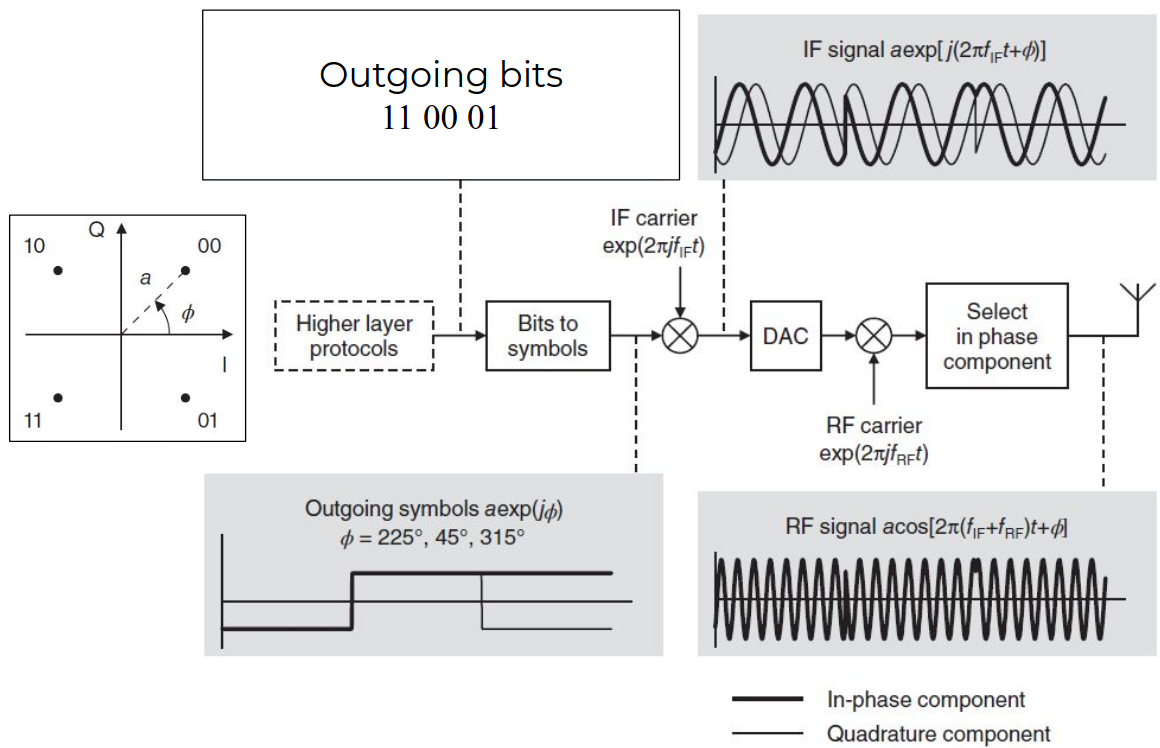
\includegraphics[width=0.9\linewidth]{img/4g/mightbesending}
\end{center}

In \textbf{ricezione}: 
\begin{itemize}
	\item si misura sull'antenna il segnale, con relativo rumore e sfasamento indotto dalla mobilità ($\psi$)

	\item rimuovo la frequenza portante, torno in banda base

	\item filtro passa-basso per eliminare il rumore termico

	\item convertitore analogico digitale (ADC)

	\item Abbiamo trasmesso $\varphi$ e ricevuto $\varphi + \psi$ (cambia di una certa sfasatura), per capire quanto è sfasato rispetto all'originale si fa channel estimation: una stima dello sfasamento dovuto al canale (condizioni del canale), fatto tramite la ricezione di un pilot standard, per poi togliere quello sfasamento dall'onda dati ricevuta

	\item conversione da simboli a bit
\end{itemize}

Le \textbf{codifiche possibili} sono:
\begin{itemize}
	\item \textbf{BPSK Binary Phase Shift Keying}: usato solo per alcuni segnali di controllo a basso livello; non importa la qualità del canale, alcuni segnali di controllo fondamentali devono essere "compresi"
	
    \item \textbf{QPSK Quadrature Phase Shift Keying}: usato per tutti i messaggi radio di controllo e trasmissione dati in caso di scarsa qualità del segnale; permette un minore overhead di controllo, mantenendo una buona "comprensibilità" del segnale
	
    \item \textbf{16/64-QAM Quadrature Amplitude Modulation}: usato per la trasmissione dati
\end{itemize}

\paragraph{Scelta di modulazione e codifica:} Si ha un Adapting Modulation e Coding scheme: quantifica la qualità del canale in 4 bit e sceglie una modulazione:
\begin{center}
	\begin{tabular}{>{\centering\arraybackslash}m{0.8cm} >{\centering\arraybackslash}m{3cm} >{\centering\arraybackslash}m{3.5cm} >{\centering\arraybackslash}m{3.5cm}}
		\toprule
		\textbf{CQI} & \textbf{Modulation scheme} & \textbf{Coding rate (units of 1/1024)} & \textbf{Information bits per symbol} \\
		\midrule
		0  & n/a     & 0   & 0.00 \\
		1  & QPSK    & 78  & 0.15 \\
		2  & QPSK    & 120 & 0.23 \\
		3  & QPSK    & 193 & 0.38 \\
		4  & QPSK    & 308 & 0.60 \\
		5  & QPSK    & 449 & 0.88 \\
		6  & QPSK    & 602 & 1.18 \\
		7  & 16-QAM  & 378 & 1.48 \\
		8  & 16-QAM  & 490 & 1.91 \\
		9  & 16-QAM  & 616 & 2.41 \\
		10 & 64-QAM  & 466 & 2.73 \\
		11 & 64-QAM  & 567 & 3.32 \\
		12 & 64-QAM  & 666 & 3.90 \\
		13 & 64-QAM  & 772 & 4.52 \\
		14 & 64-QAM  & 873 & 5.12 \\
		15 & 64-QAM  & 948 & 5.55 \\
		\bottomrule
	\end{tabular}
\end{center}

Esempio: con CQI 7 si hanno 1.48 bit di informazione per ogni simbolo, quindi per 1024 bit 378 saranno di informazione. Queste valgono per il data plane, il control plane ha una sua codifica molto meno variabile.

\subsubsection{Riuso frequenze}
\begin{center}
	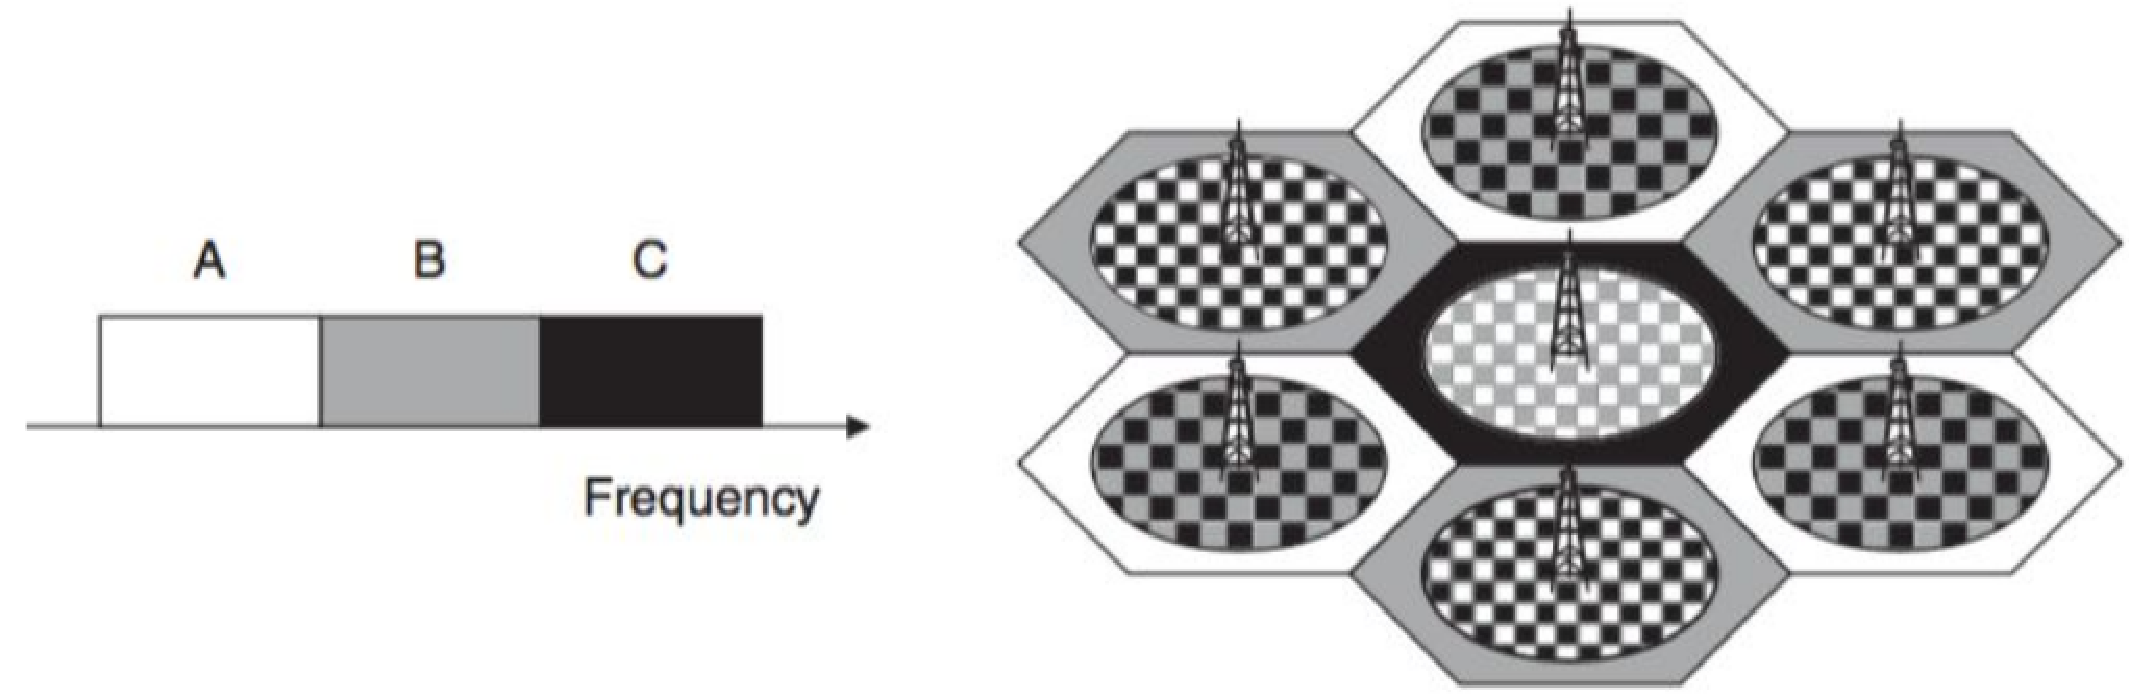
\includegraphics[width=0.9\linewidth]{img/4g/riuso4g}
\end{center}

Si utilizza il 100\% delle frequenze disponibili, come in UMTS, ma rispetto a quest'ultimo la gestione delle interferenze è più semplice e coordinata tra le celle tramite l’apposita interfaccia X2. Le frequenze vengono coordinate ai bordi delle celle, in modo da usare una banda maggiore al centro, dove non possono esserci interferenze; ai bordi delle celle le frequenze sono diverse tra celle adiacenti, al centro viene usata la banda completa.

\subsubsection{Durata Simboli}

Non è casuale, è decisa in base a
\begin{itemize}
	\item la distanza tra sottoportanti $15kHz$

	\item punti da campionare per la trasformata di Fourier $2048$
\end{itemize}

Di conseguenza
$$ T_S = \frac{1}{2048 \cdot 15000}s \approx 32.6 ns $$

Quindi il processore fisico deve avere una velocità adeguata. Un simbolo dura $2048 T_S = 66.7 \mu s$.

\subsubsection{Struttura Slot}

I simboli sono organizzati in slot da $0.5ms$ ($15360 T_S$).

Si ha un cyclic prefix per evitare interferenza inter-simbolo causa del multipath. 

Per ogni slot ci sono 7 simboli ($66.7 \mu s$ ognuno), di cui $4.7$ o $5.2 \mu s$ sono di preambolo.

\begin{center}
	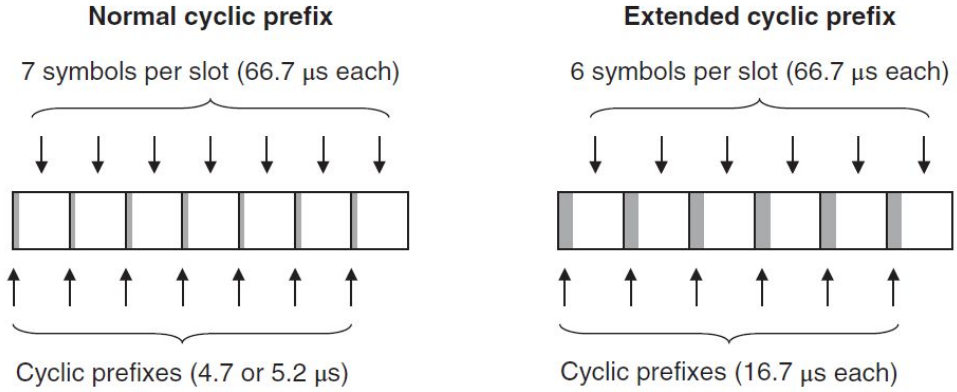
\includegraphics[width=0.85\linewidth]{img/4g/cycprefix}
\end{center}

\subsubsection{Duplex}

Per la gestione del duplex, ogni eNodeB può essere configurato in una di 2 modalità, comunicate allo UE durante la fase di configurazione: 
\begin{itemize}
	\item \textbf{Frequency Division Duplex (FDD)}: Utilizzo di frequenze diverse per uplink e downlink
	\begin{center}
		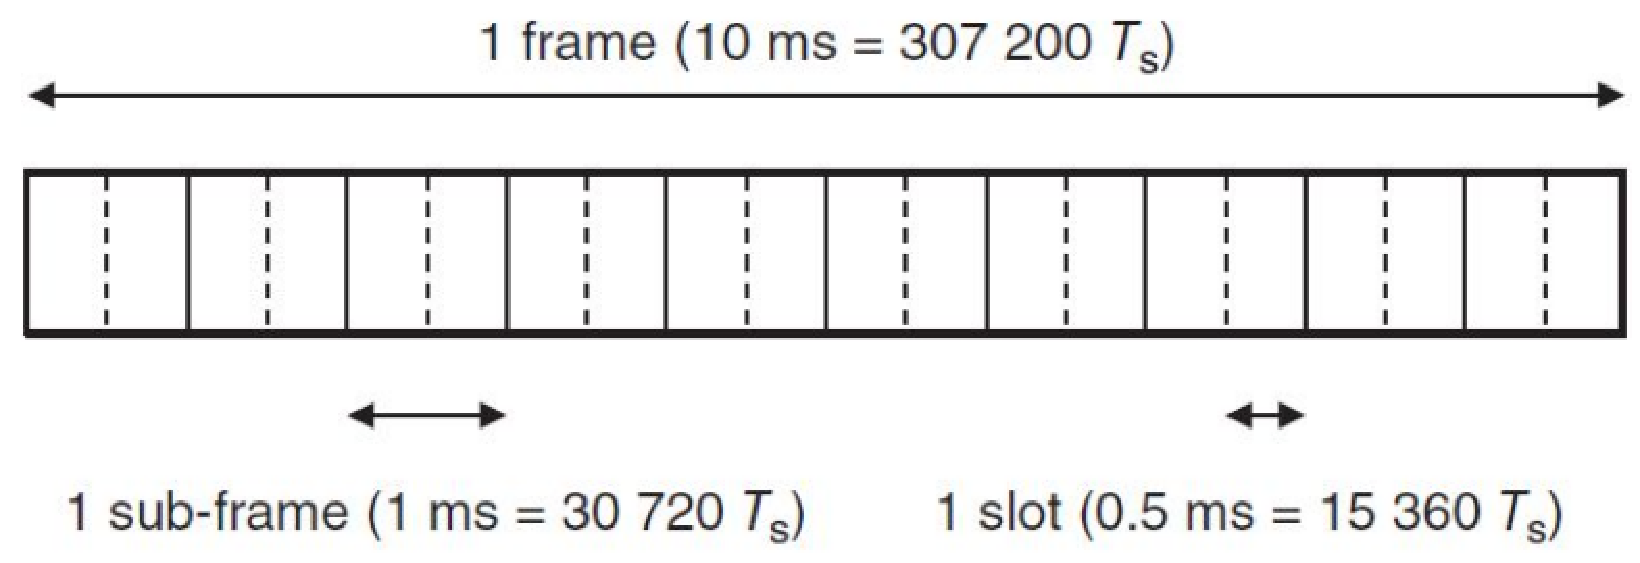
\includegraphics[width=0.5\linewidth]{img/4g/fdd}
	\end{center}
	ogni frame di $10ms = 307200 T_S$ contiene 10 subframe/20 slot da $1/0.5ms$, quindi si hanno 140 simboli/frame (20x7) con normal cyclic prefix e 120 simboli/frame (20x6) con extended cyclic prefix.
	
	\item \textbf{Time Division Duplex (TDD)}: Utilizzo di una sola frequenza per uplink e downlink. Sono possibili 7 configurazioni:
	\begin{center}
		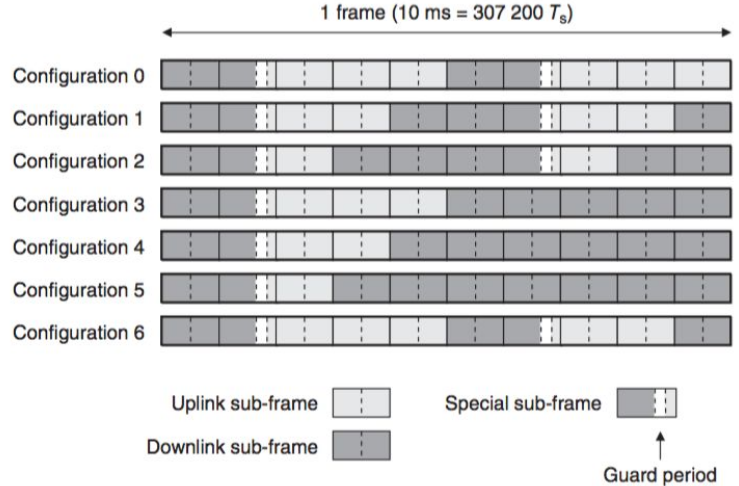
\includegraphics[width=0.7\linewidth]{img/4g/tdd}
	\end{center}
	La configurazione è decisa in base all'utilizzo (se serve più downlink ne metto di più, o viceversa).
\end{itemize}

\paragraph{Uplink Timing Advance:} Il guard period tiene conto dell'anticipo di trasmissione in uplink (Uplink Timing Advance). UE inizia a trasmettere in uplink in anticipo rispetto al tempo del frame della base station, altrimenti la ricezione avverrebbe in maniera disallineata dal tempo degli slot della BS, dato che dispositivi più lontani ci mettono più tempo a far arrivare il segnale. 

Viene fornito un range di timing advance tra $0$ e $667\mu s$ per compensare la distanza. Per fare questo serve però che nessuno stia parlando in downlink durante il tempo di advance (altrimenti si avrebbe interferenza), per questo il guard time: serve a permettere l'advance per l'uplink senza interferenze.

Il timing advance garantisce che, anche con le differenze dovute alla propagazione, i simboli arrivino entro il cyclic prefix, mantenendo la divisione di slot temporali.

\subsubsection{Orthogonal Frequency Division Multiple Access OFDMA}

Gli eNodeB usano \textbf{OFDMA}: la banda viene divisa in piccole sotto-bande (sub-carriers) le cui frequenze non causano interferenze. LTE usa sotto-bande di ampiezza $15 kHz$ (frequenze intermedie IF di modulazione ortogonali). 

Più sotto-bande sono organizzate in \textbf{Resource Block} che rappresentano la minima quantità di risorse allocabili a un singolo dispositivo.

\begin{center}
	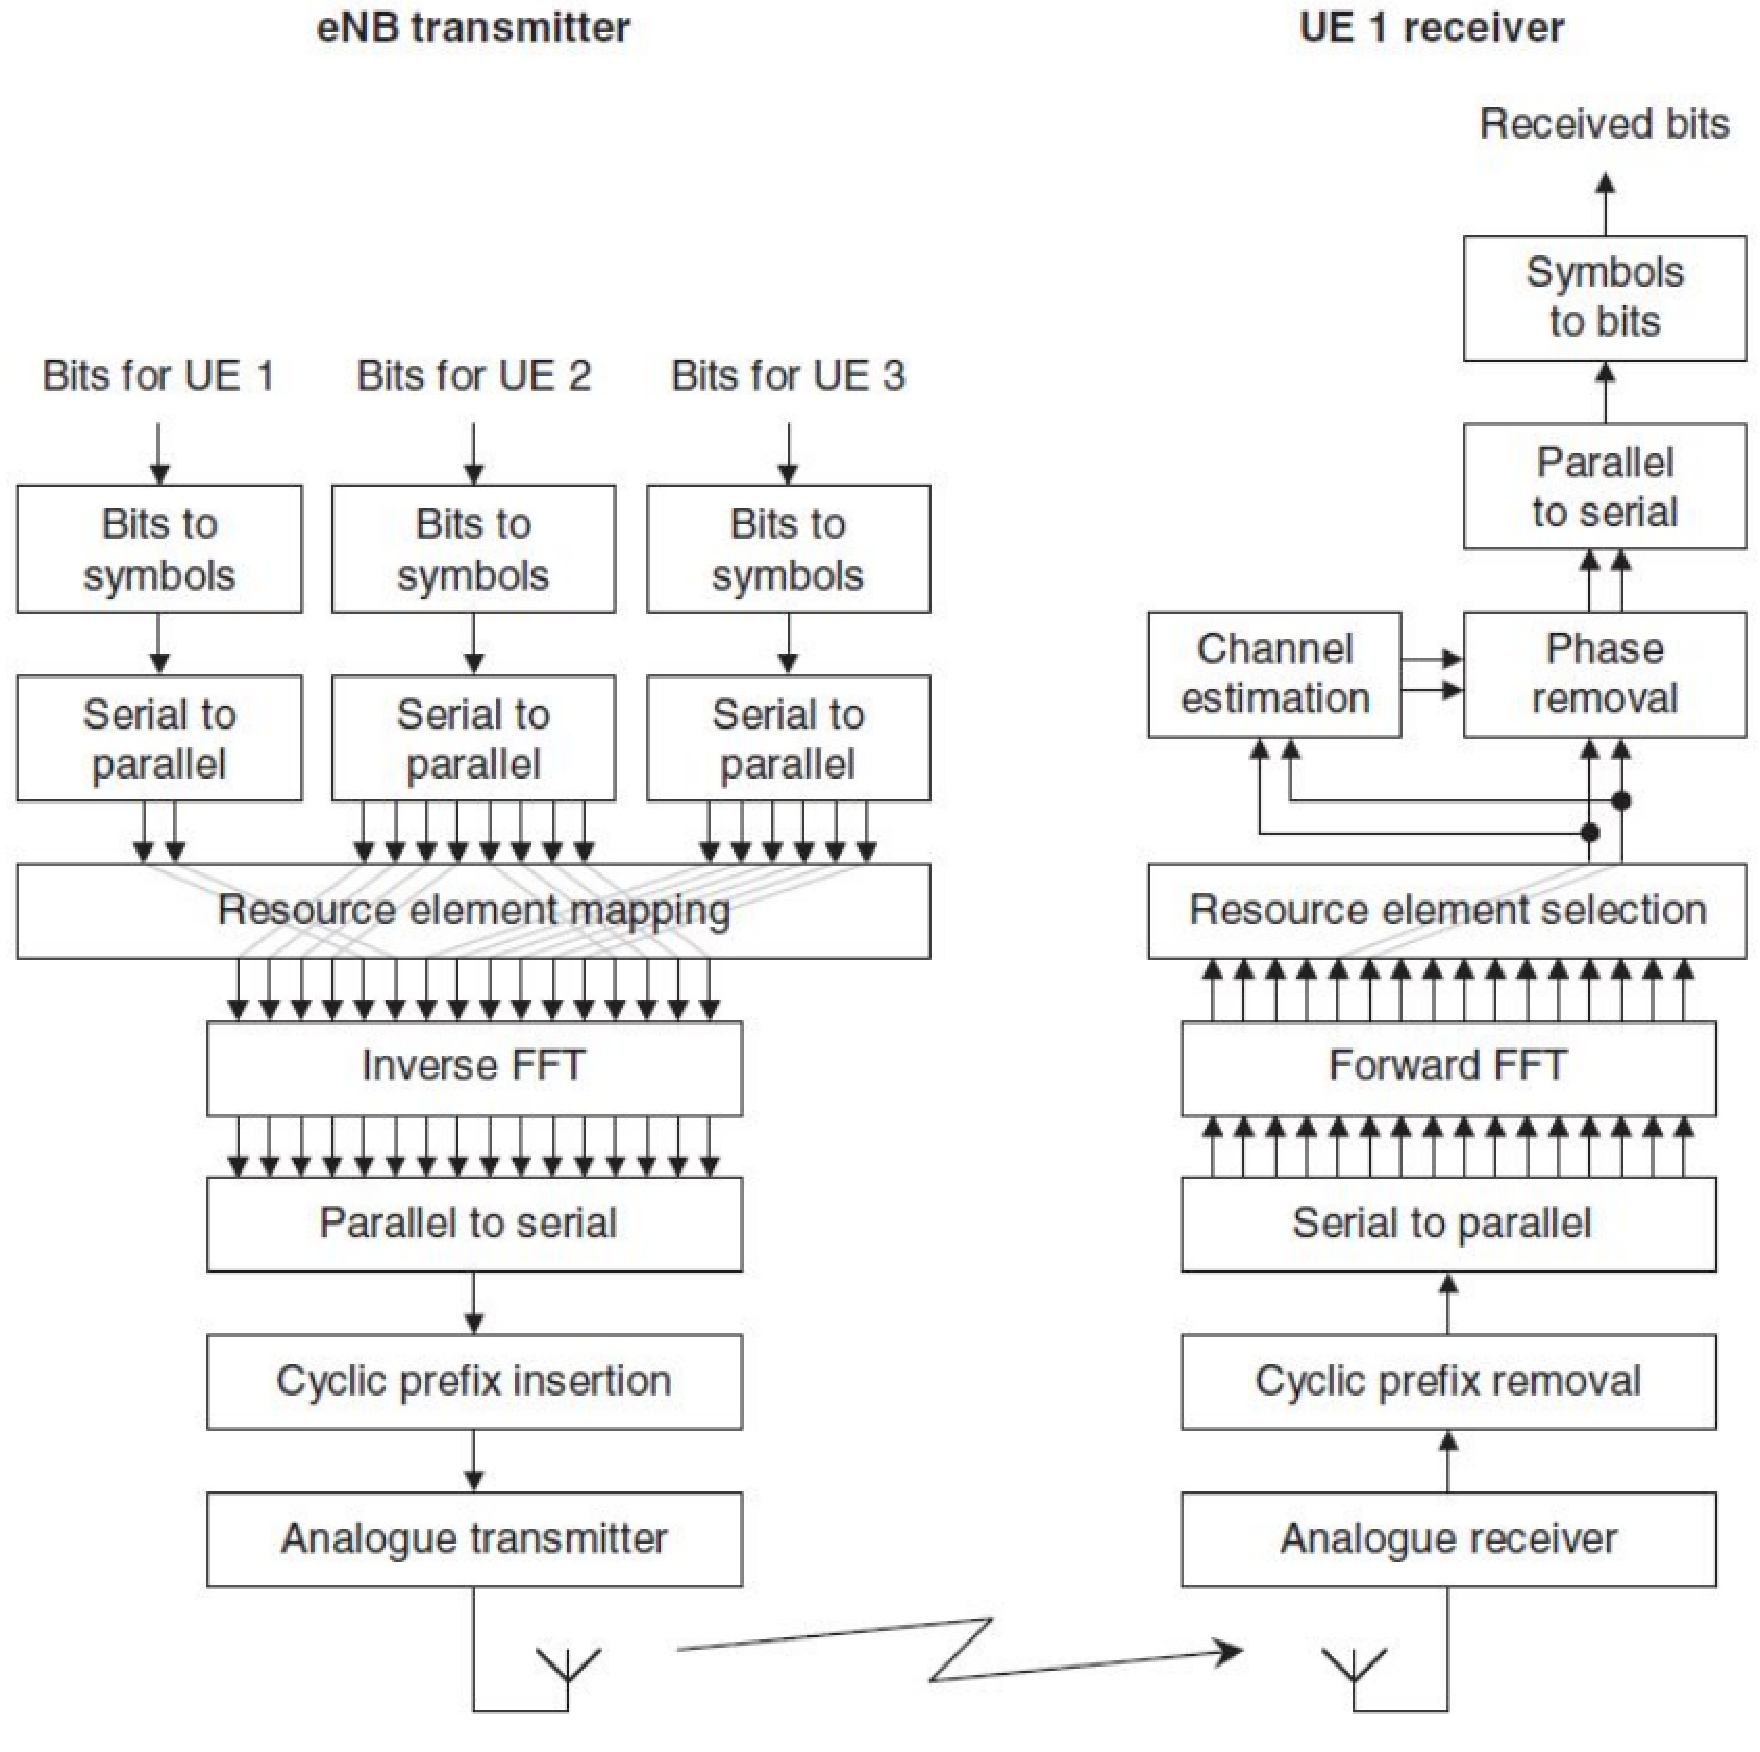
\includegraphics[width=0.85\linewidth]{img/4g/utranofdma}
\end{center}

Gli step lato trasmettitore sono: 
\begin{itemize}
	\item Ogni flusso di bit distinto viene trasformato in simboli

	\item I simboli vengono mappati sulle risorse in frequenza (resource block allocati)

	\item Si applica la IFFT per trasformare i simboli mappati in frequenza nel dominio del tempo, ottenendo il segnale OFDM complesso

	\item I campioni temporali paralleli vengono ricombinati in un unico flusso seriale

	\item Si aggiunge il prefisso ciclico

	\item Il segnale viene convertito in analogico e trasmesso
\end{itemize}

Lato ricevitore bisogna fare il processo contrario, estraendo il flusso di bit per l'UE che sta ricevendo (sceglie di considerare solo i resource block a lui dedicati), correggendo il flusso dal rumore e sfasamento (tramite channel estimation).

Si hanno 12 sotto-bande di larghezza minima $180 kHz$ e 7 simboli in $0.5ms$. 

\subsubsection{eNodeB Scheduler}

Tutte le comunicazioni da e per i dispositivi sono gestite dall'eNodeB. Lo scheduling ha risorse a disposizione (resource blocks) e determina come allocarli
\begin{center}
	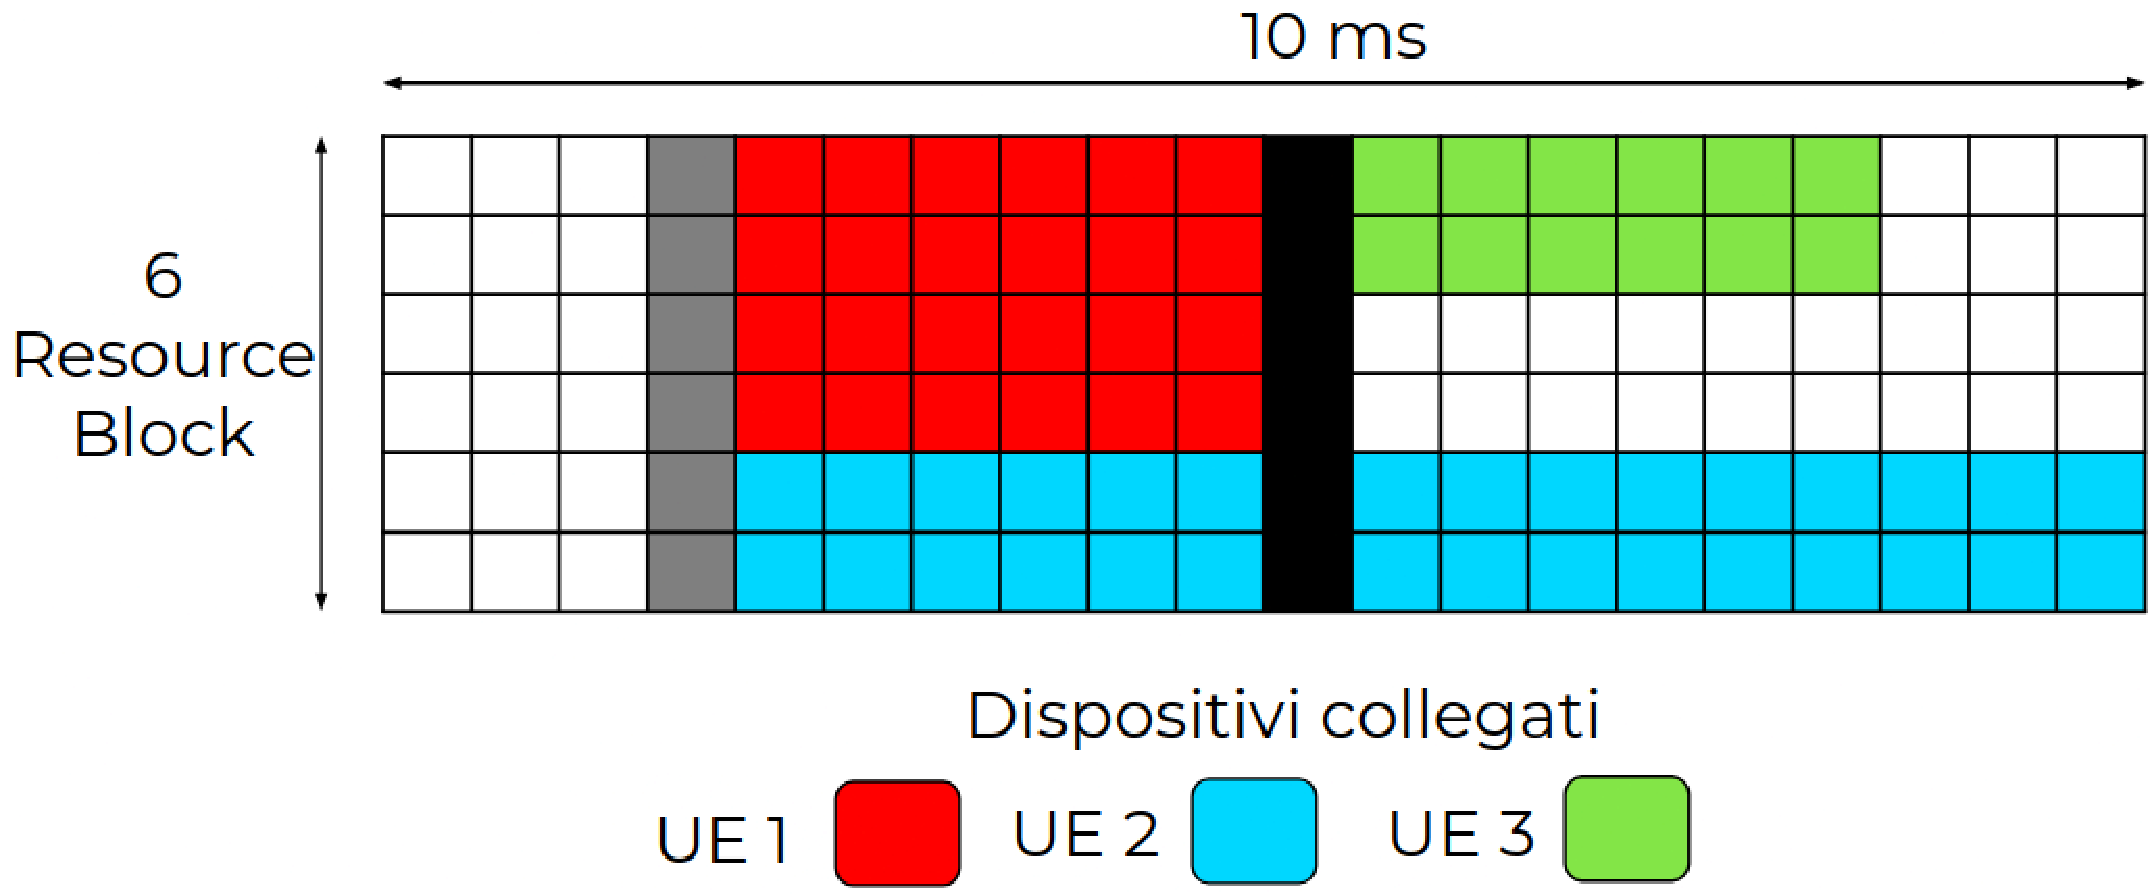
\includegraphics[width=0.75\linewidth]{img/4g/alloc}
\end{center}

Blocchi grigi e neri sono dedicati alla trasmissione della BS. Tutto lo scheduling deve essere fatto real time (i.e., molto veloce).

\subsubsection{Velocità per UE}

Alla fine la banda disponibile per ogni singolo dispositivo dipende da molti fattori: 
\begin{itemize}
	\item Capacità del dispositivo (UE)

	\item Qualità del segnale radio: interferenze e distanza, determina la scelta della codifica

	\item Larghezza della banda in $MHz$: maggiore banda, maggior numero di resource block allocabili

	\item Configurazione TDD: a seconda della configurazione dell'eNodeB si possono avere differenti velocità di upload e download

	\item Numero dispositivi collegati

	\item Altri fattori non dipendenti dal canale radio: come congestione della rete di backhaul, congestione P-GW o altri fattori end-to-end
\end{itemize}

Le massime velocità teoriche per LTE Rel8 sono $300Mbps$ in download e $75Mbps$ in upload.

%End L17

\subsubsection{Collegamento alla Core Network}

Oltre al collegamento alla core network tramite S1, si aggiunge un collegamento diretto tra BS, tramite un'interfaccia denominata X2, con una suite di protocolli dedicata. Questo permette di svolgere compiti locali tra le BS.

Schema logico e fisico:
\begin{center}
	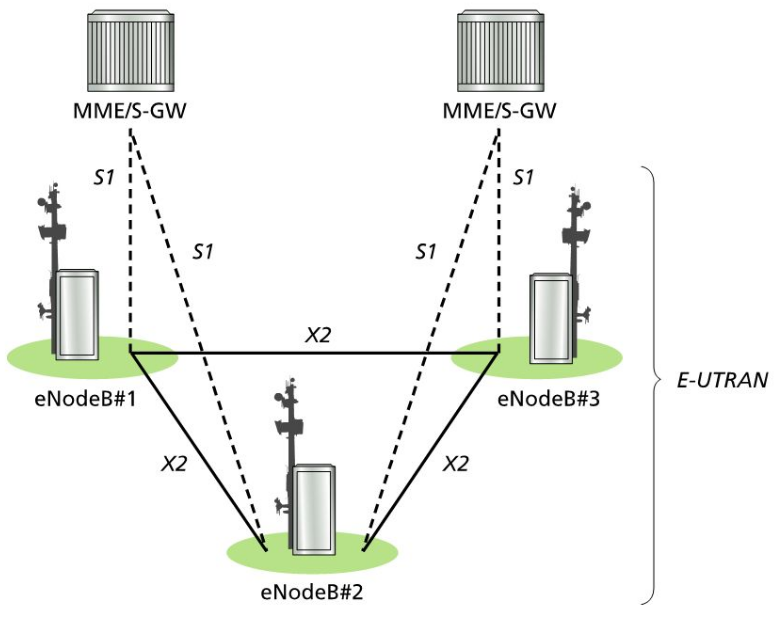
\includegraphics[width=0.6\linewidth]{img/4g/x21}
\end{center}

\subsubsection{Tracking Area}

Per questioni di fault tolerance, ridondanza e load balancing si ha un \textbf{raggruppamento delle BS in Tracking Areas TAs}. Può essere visto come un cluster di BS. A ciascuno di questi cluster sono associati uno o più gruppi di moduli di controllo.
\begin{center}
	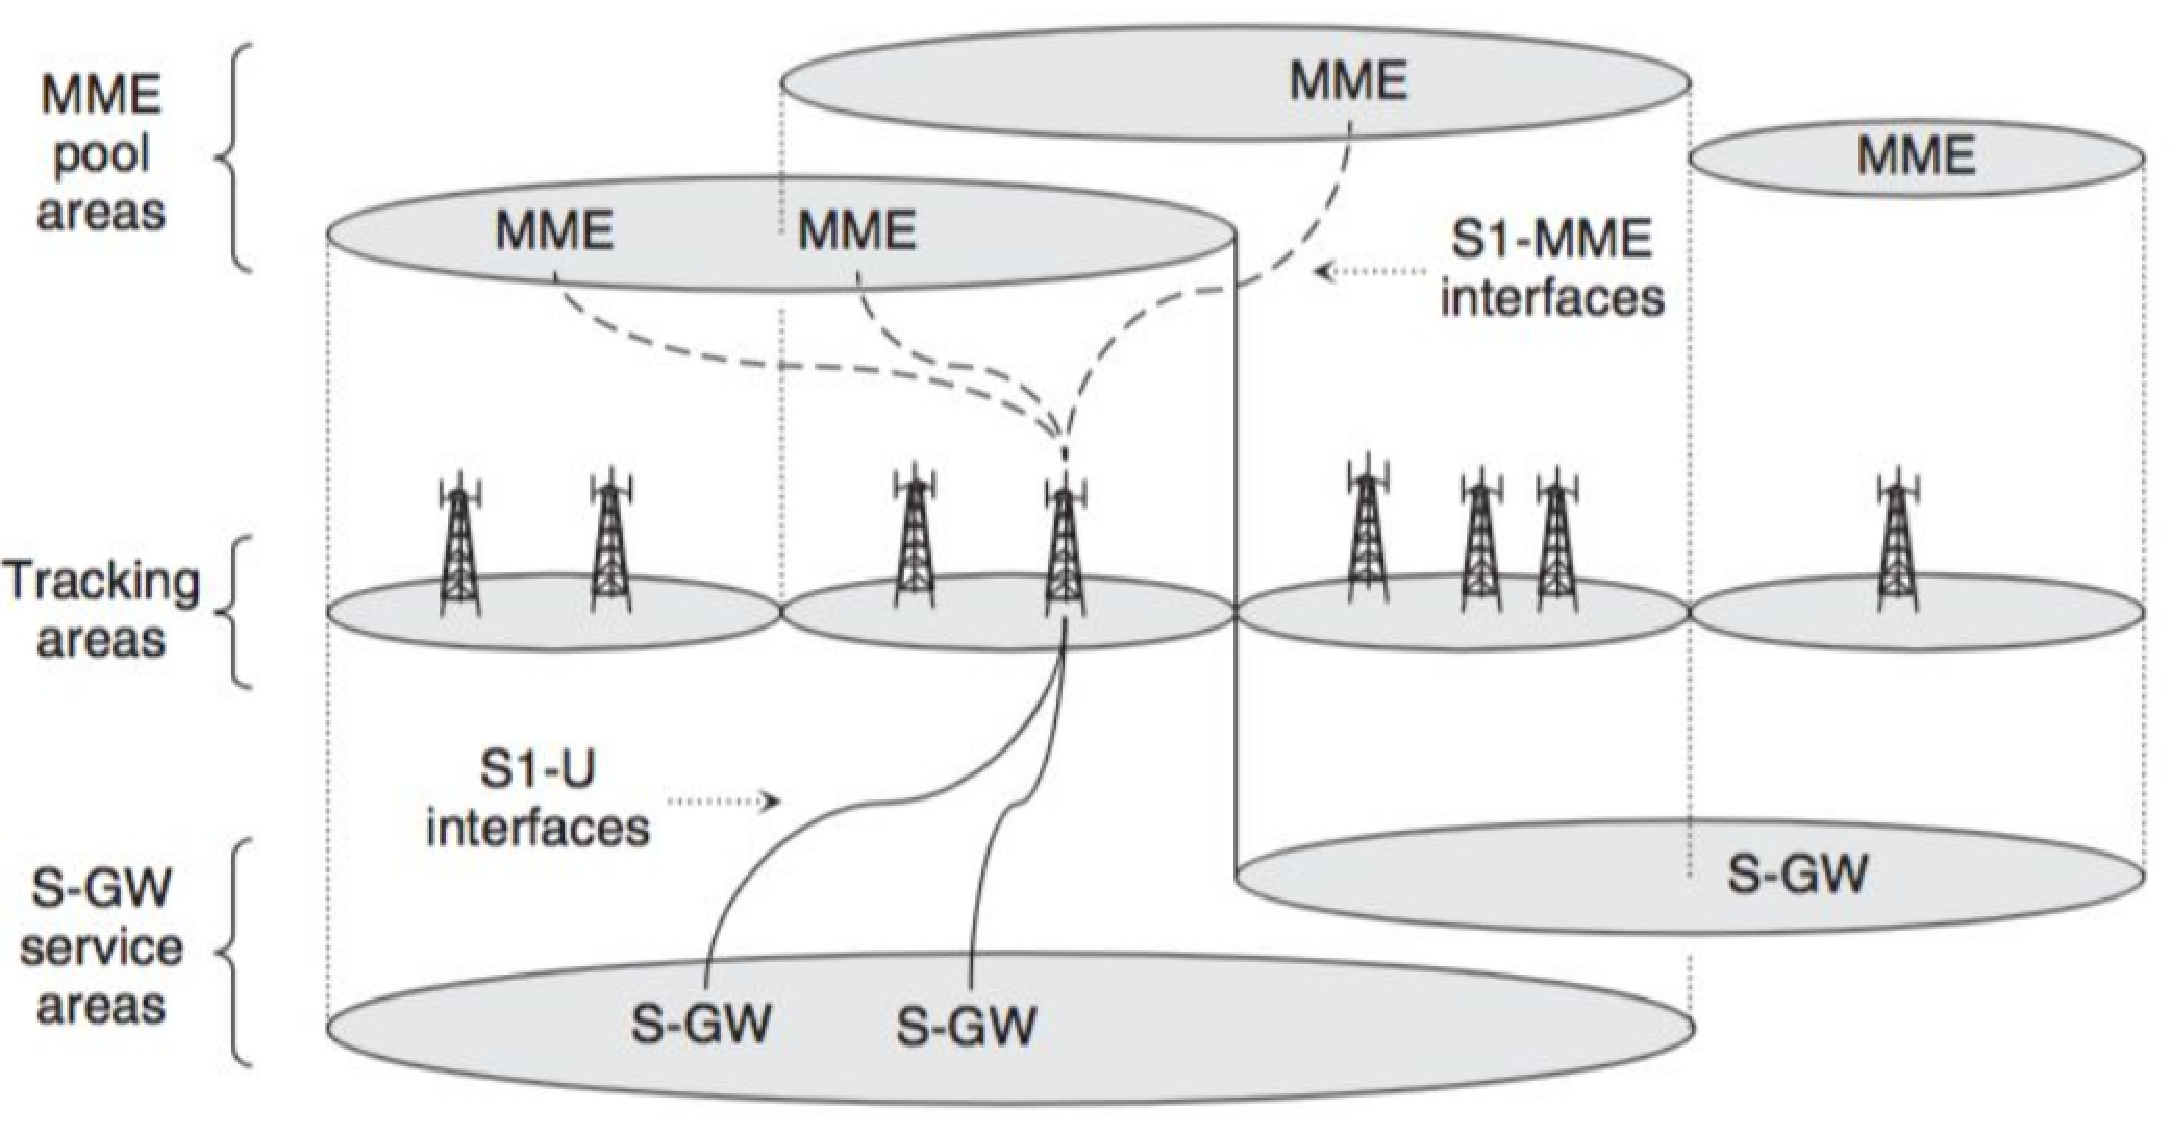
\includegraphics[width=0.7\linewidth]{img/4g/tas}
\end{center}

\subsubsection{Interfaccia X2}

La suite di protocolli dell'interfaccia X2 permette la \textbf{comunicazione diretta tra eNodeB}. Permette: 
\begin{itemize}
	\item gestione handover in alternativa a S1

	\item funzionalità Self-Organizing Network (SON): load balancing, gestione delle interferenze

	\item mantenimento dello storico delle ultime celle visitate per gestire l'effetto Ping-Pong tra celle
\end{itemize}

In generale, oltre a essere un canale di handover alternativo, permette meccanismi SON, coordinazione radio, load balancing dinamico e altre funzionalità per migliorare l'efficienza della rete.

\subsection{Architettura}

\subsubsection{Control Plane}

Si ha una netta separazione tra control e data plane. I moduli direttamente coinvolti nel control plane sono UE, eNodeB e MME.

Lo \textbf{stack} di protocolli è:
\begin{center}
	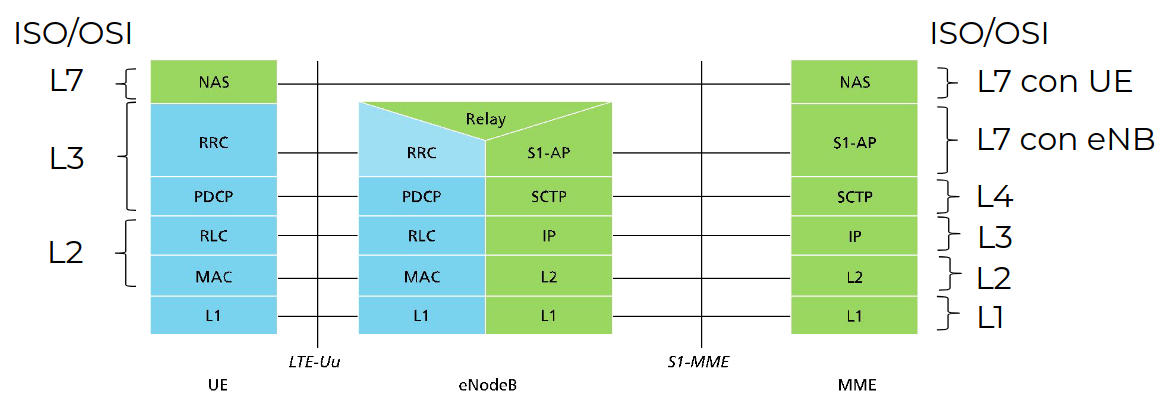
\includegraphics[width=0.99\linewidth]{img/4g/cps}
\end{center}

A lato indicato l'equivalente ISO/OSI. La BS è dual stack in quanto deve parlare con entrambi i lati. Livello 1 e 2 non sono specificati in quanto "a scelta".

\paragraph{UE - eNodeB:} A sinistra c'è la parte di UE, i protocolli (dall'alto verso il basso) sono:
\begin{itemize}
	\item \textbf{Radio Resource Control RRC}:
	\begin{itemize}
		\item gestisce il paging, le informazioni di paging passano per questo livello
	
    	\item gestisce la mobilità, viene deciso l'handover
	
    	\item si occupa di QoS e raccolta misurazioni UE
	\end{itemize}
	
	\item \textbf{Packet Data Convergence Protocol PDCP}:
	\begin{itemize}
		\item convergenza tra mondo IP e mobile, comprime gli header, mandando di fatto solo le differenze
	\end{itemize}
	
	\item \textbf{Radio Link Control RLC}:
	\begin{itemize}
		\item correzione errori
	
    	\item gestione ritrasmissione
	
    	\item segmentazione/riassemblaggio dei pacchetti dei livelli superiori
	\end{itemize}
	
	\item \textbf{Medium Access Control MAC}:
	\begin{itemize}
		\item gestione dell'accesso al canale radio
	
    	\item gestione dello scheduler (da eNodeB)
	\end{itemize}
\end{itemize}

\paragraph{eNodeB - MME:} L'altro lato include: 
\begin{itemize}
	\item \textbf{Livello applicazione interfaccia S1 S1-AP}:
	\begin{itemize}
		\item trasporto di tutto il traffico di controllo tra E-UTRAN e Core Network
	\end{itemize}
	
	\item \textbf{Stream Control Transmission Protocol SCTP}: 
	\begin{itemize}
		\item protocollo di livello trasporto utilizzato per ottimizzare il trasporto del traffico di segnalazione
	\end{itemize}
	
	\item \textbf{Internet Protocol IP} (interno alla rete operatore):
	\begin{itemize}
		\item eNB: indirizzo IP interno alla rete operatore per identificare uno specifico eNB nella rete
	
    	\item MME: indirizzo IP interno alla rete che identifica uno specifico MME nella rete
	
    	\item Il routing dei messaggi control plane
	\end{itemize}
\end{itemize}

\paragraph{SCTP - Motivazioni:} Le motivazioni dietro l'uso di SCTP sono:
\begin{enumerate}
	\item TCP fornisce solo trasporto affidabile e in ordine: la consegna è solo affidabile e non permette ordine parziale
	
    \item Head of Line Blocking Problem
	
    \item TCP è stream oriented, le applicazioni aggiungono marker specifici per delimitare i messaggi
	
    \item Supporto Multi-Homing mancante: le connessioni sono esclusivamente da e verso una singola entità
\end{enumerate}

\paragraph{Head of Line HOL Block Problem:} In TCP tutto deve essere \textit{in ordine}, ogni messaggio ricevuto può essere passato al livello superiore se e solo se il segmento è in ordine rispetto agli altri (sono stati correttamente ricevuti tutti i messaggi precedenti). Se viene perso un segmento, i pezzi successivi sono bufferati ma non possono essere passati al livello applicativo.

Applicato al collegamento eNodeB-MME vorrebbe dire avere un flusso unico per i dati di tutti i dispositivi collegati alla BS. 
\begin{center}
	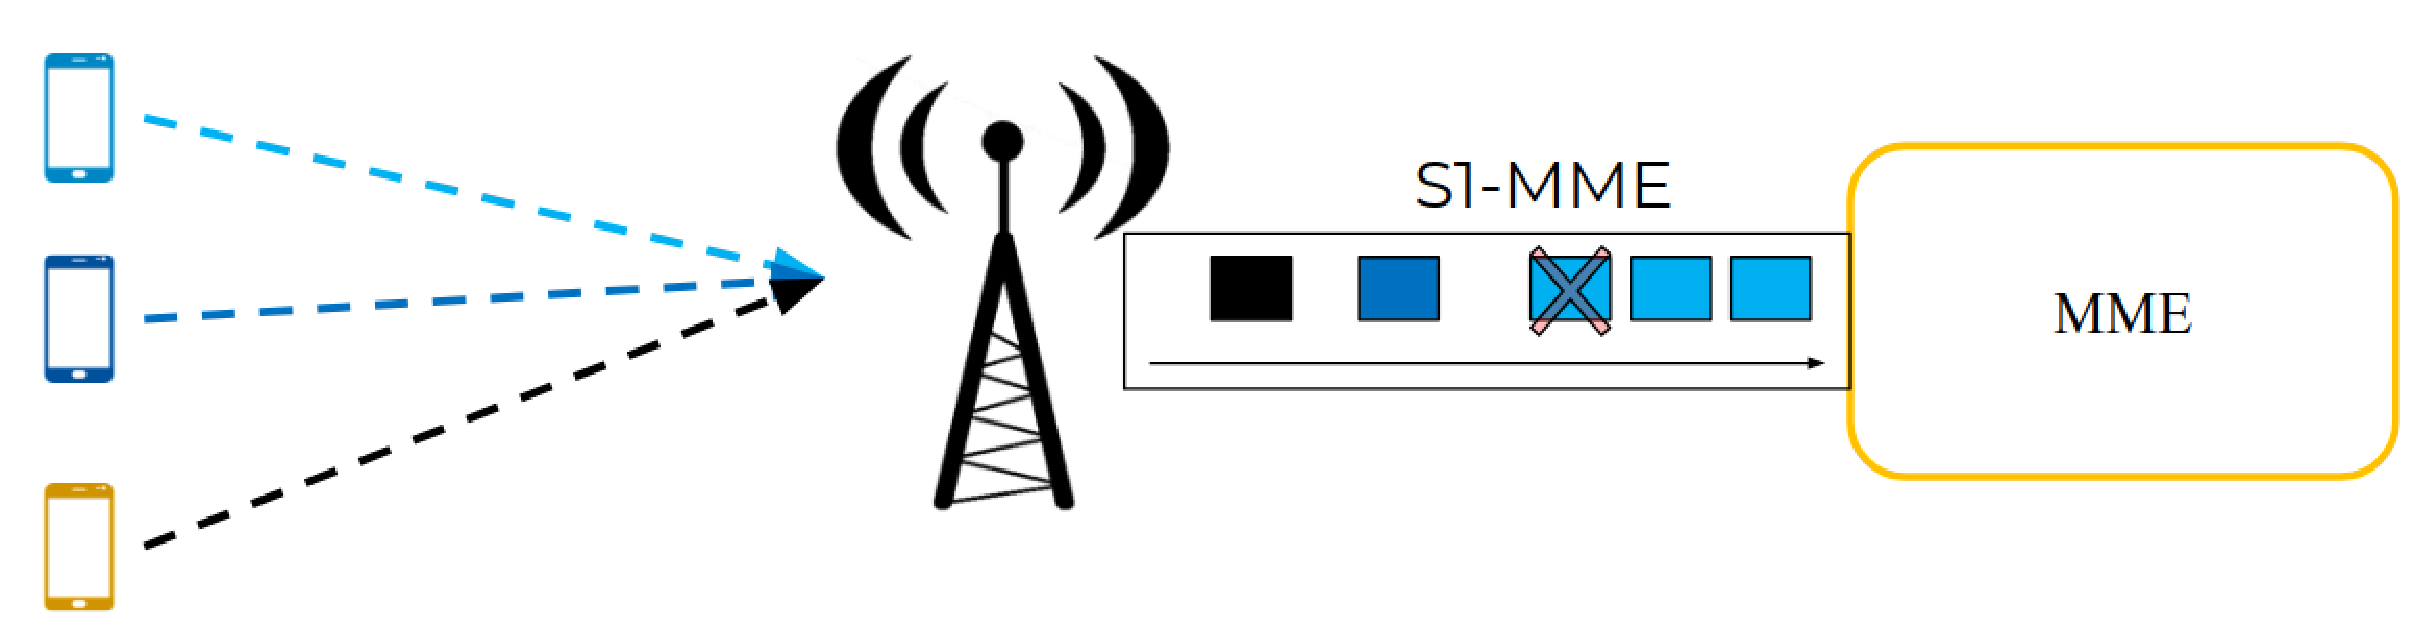
\includegraphics[width=0.7\linewidth]{img/4g/holprob1}
\end{center}

Tutti i pacchetti fanno parte di un cumulative ack e la perdita di un pacchetto vorrebbe dire bloccare tutti gli altri. Non rende indipendenti tra loro i dispositivi collegati alla eNodeB (e non dovrebbero avere dipendenze).

Una prima soluzione potrebbe essere aprire connessioni separate per ogni dispositivo gestito dall'eNodeB: soluzione non abbastanza scalabile, utilizza troppe risorse (dell'MME principalmente, una porta per dispositivo su tutte le BS che gestisce è decisamente troppo).

La \textit{vera} soluzione è usare \textbf{SCTP}: viene aggiunto uno \textbf{stream ID} (16 bit) ai pacchetti, definendo \textbf{multipli stream} all'interno di una \textbf{singola connessione}. 

Se viene perso un pacchetto, vengono bloccati solo i pacchetti con lo stesso stream ID, non gli altri. Una singola connessione ha al suo interno più stream indipendenti, ognuno dei quali contiene dati completamente separati. Orientato alla connessione e affidabile, garantisce che i pacchetti arrivino a destinazione in ordine (anche parziale, ordine dello stream, non totale).

SCTP permette anche il \textbf{Multi-Homing}: non viene usata la quadrupla tipica di TCP, ma l'identificazione della connessione viene fatta tramite gruppi di indirizzi sorgente e destinazione. Identificatori:
\begin{center}
	\begin{tabular}{l l}
		TCP & <SRC Address, SRC Port, DST Address, DST Port> \\
		SCTP & < \textbf{\{SRC Addresses\}}, SRC port, \textbf{\{DST Addresses\}}, DST port>
	\end{tabular}
\end{center}

TCP aggiunge delimitatori e richiede parsing dei messaggi a livello di applicazione, in quanto stream oriented. SCTP invece è \textbf{Message Oriented} (come UDP), divide i singoli messaggi, si occupa di gestire frammentazione, gestione di flusso e di errori.

\paragraph{Confronto SCTP-TCP-UDP:}
\begin{center}
	\begin{tabular}{lccc}
		\toprule
		\textbf{Feature} & \textbf{SCTP} & \textbf{TCP} & \textbf{UDP} \\
		\midrule
		Message‐Oriented                              & X &   & X \\
		Byte‐Oriented                                 &   & X &   \\
		Connection‐Oriented                           & X & X &   \\
		Full‐Duplex                                   & X & X & X \\
		Trasporto affidabile                          & X & X &   \\
		Consegna in ordine                            & X & X &   \\
		Consegna NON in ordine               & X &   & X \\
		Controllo di flusso e di congestione          & X & X &   \\
		ECN (Explicit Congestion Notification)        & X &   &   \\
		Multi‐Streaming                               & X &   &   \\
		Multi‐Homing                                  & X &   &   \\
		Prevenzione SYN flooding attack               & X &   &   \\
		\bottomrule
	\end{tabular}
\end{center}

\subsubsection{User Plane}

I moduli coinvolti nell'user plane sono: UE, eNodeB, S-GW, P-GW, servizi operatore.

Lo \textbf{stack} è 
\begin{center}
	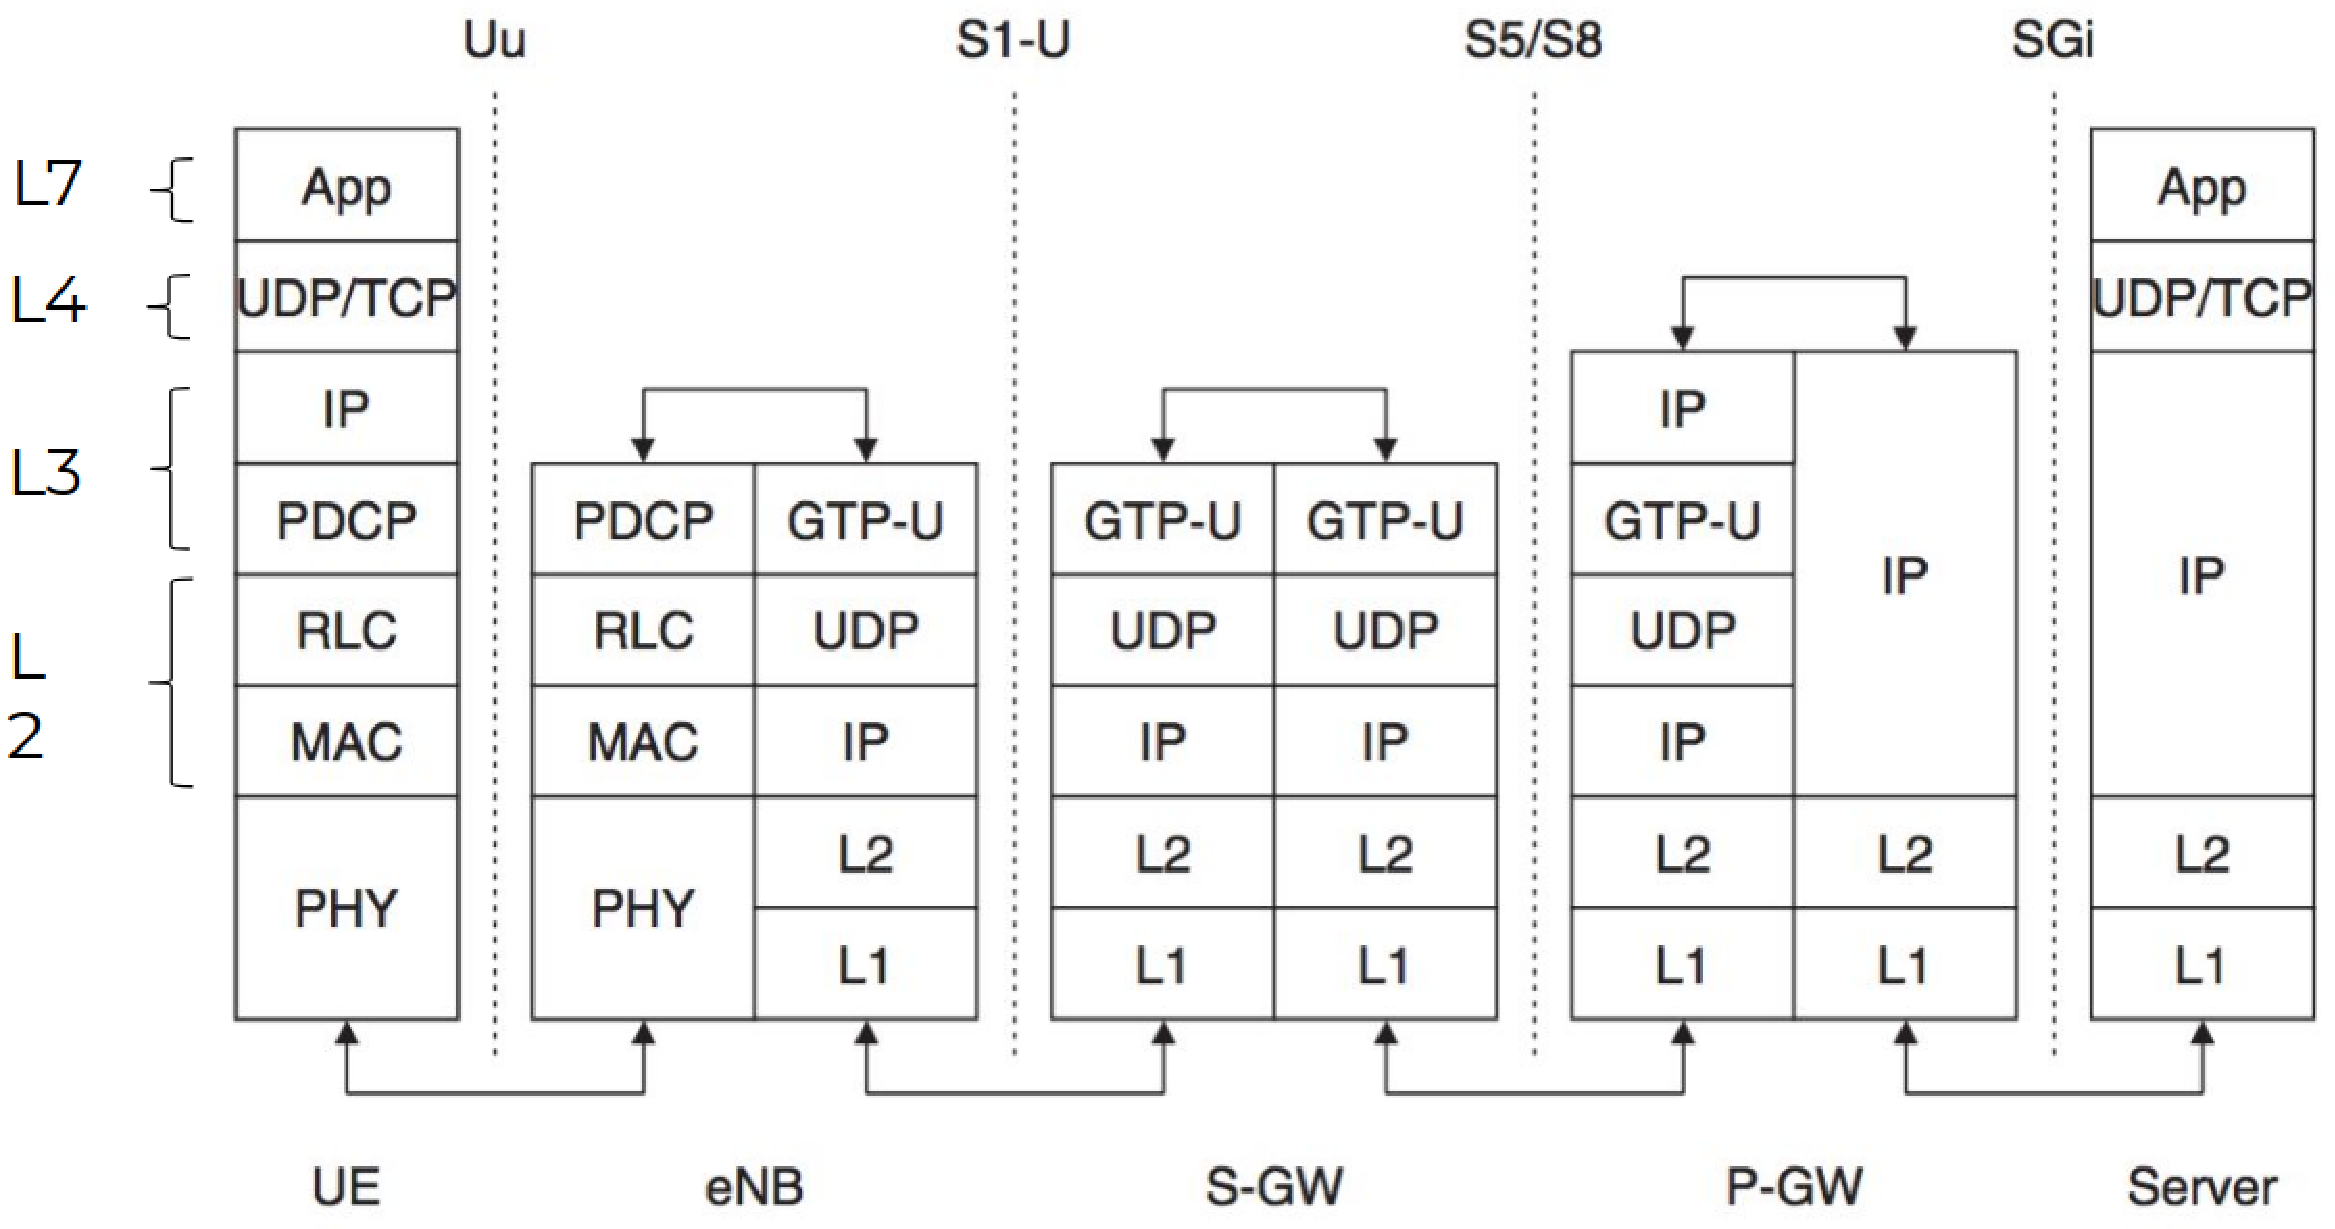
\includegraphics[width=0.95\linewidth]{img/4g/ups}
\end{center}

\paragraph{UE - eNodeB:} I primi 4 livelli sono uguali al control plane (PHY, MAC, RLC, PDCP), mentre sopra si ha uno stack IP "classico".

Ci sono diversi protocolli IP, ognuno con il suo motivo: 
\begin{itemize}
	\item tra UE e P-GW: indirizzo IP interno, valido per tutta la connessione tra UE e P-GW, assegnato con DHCP e "nascosto" con NAT
	
    \item tra P-GW e server (internet, mondo esterno): indirizzo IP pubblico del P-GW, indirizzo IP pubblico del server; per "collegarlo" all'indirizzo IP interno viene usato il NAT
	
    \item tutti quelli sotto: indirizzi IP della rete interna dell'operatore
\end{itemize}

\subsubsection{GPRS Tunneling Protocol GTP} 

La connessione logica tra UE e PGW è identificata da una sessione Packet Data Network (PDN).  Lo UE è libero di muoversi all'interno della rete e possiede un proprio IP unico all'interno della rete (DHCP/NAT), mantenuto per tutta la durata della sessione. 

eNodeB e SGW possono cambiare durante la durata della connessione. Ogni volta che un dispositivo cambia connessione bisognerebbe cambiare le tabelle di routing:  impossibile da gestire in scala, o comunque troppo dispendioso. 

La rete è generalmente fissa (le eNodeB cambiano \textit{raramente}), l'unica parte che cambia spesso sono i collegamenti finali (i dispositivi utente).

Il pacchetto che parte dall'UE e gestito dall'eNodeB tramite l'interfaccia Uu è 
\begin{center}
	\begin{tabular}{l | C{1cm} | C{1cm} | C{1cm} | C{1cm} |}
		\cline{2-5}
		UE $\leftrightarrow$ eNodeB & RLC & IP & UPD/ TCP & DATA \\
		\cline{2-5}
	\end{tabular}
\end{center}

Mentre il pacchetto gestito dall'eNodeB tramite interfaccia S1-U viene incapsulato GTP:
\begin{center}
	\begin{tabular}{| C{1.5cm} | C{1.7cm} | C{2cm} | C{1.2cm} | C{1.2cm} | C{1.2cm} |}
		\multicolumn{1}{C{1.5cm}}{IP SGW} & \multicolumn{1}{C{1.7cm}}{UDP port SGW} & \multicolumn{1}{C{2cm}}{Tunnel ID (TEID)} & \multicolumn{3}{C{3.6cm}}{Pacchetto Utente \newline Incapsulamento GTP} \\
		\hline
		IP & UDP & GTP & IP & UDP/ TCP & DATA \\
		\hline
	\end{tabular}
\end{center}

Quando passa dalla eNodeB a SGW: la prossima destinazione è il PGW, quindi: 
\begin{itemize}
	\item IP SGW $\rightarrow$ IP PGW 

	\item UDP Port SGW $\rightarrow$ UDP Port PGW

	\item Il TEID prima faceva riferimento alla connessione eNodeB $\leftrightarrow$ SGW, adesso a SGW $\leftrightarrow$ PGW
\end{itemize}

Al gateway viene rimosso l'incapsulamento NAT e GTP, prima di essere consegnato alla rete esterna.
\begin{center}
	\renewcommand{\arraystretch}{1.4}
	\begin{tabular}{| C{3cm} | C{3cm} | C{3cm} |}
		\multicolumn{3}{C{9cm}}{Pacchetto Utente \newline Rimozione incapsulamento GTP e NAT} \\
		\hline
		IP & UDP/TCP & DATA \\
		\hline
	\end{tabular}
\end{center}

L'operatore nasconde completamente la mobilità (a livello di trasferimento dati) al mondo esterno, tutti i dati passano dal P-GW.

\subsection{LTE EPS Bearers}

Si può astrarre a più livelli i bearer usati nella rete:

\begin{center}
	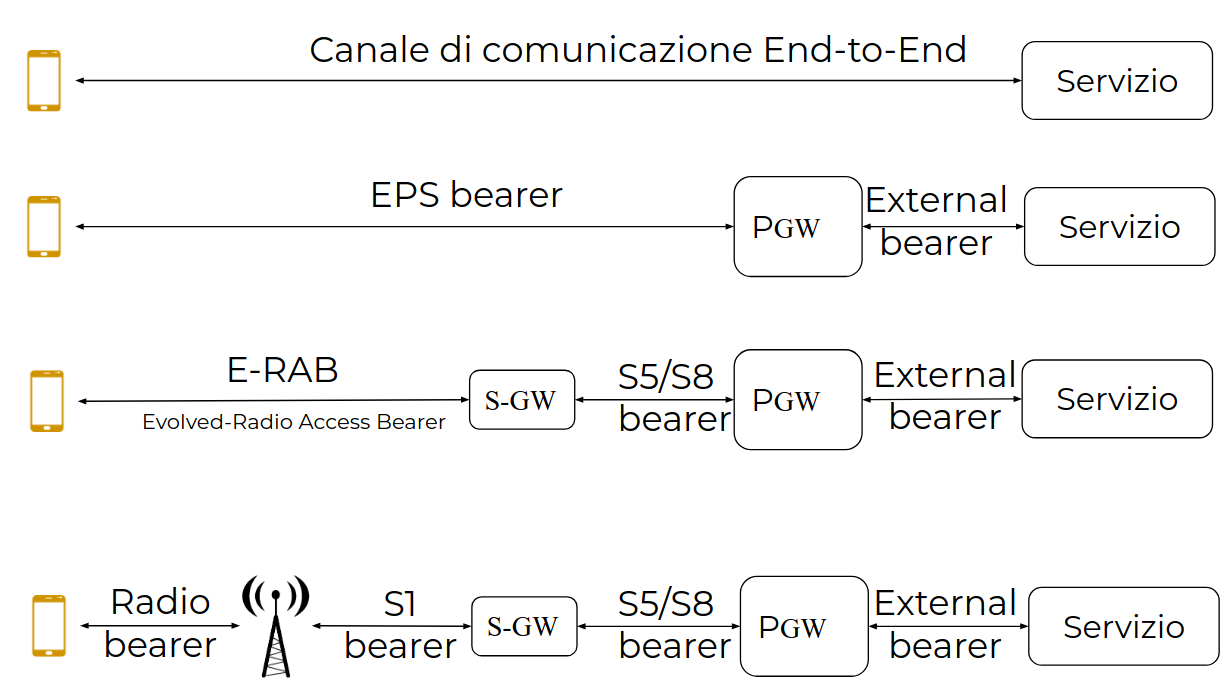
\includegraphics[width=0.8\linewidth]{img/4g/bearing}
\end{center}

Cambiare l'antenna a cui un dispositivo è collegato non richiede necessariamente di cambiare tutti i bearer: 
\begin{itemize}
	\item sicuramente cambierà il radio bearer (l'antenna a cui è collegato è diversa)
    
	\item cambierà l'S1 bearer se l'antenna fa parte di una nuova BS

	\item il bearer S5/S8 cambierà solo se la nuova BS fa parte di un alrto SGW

    \item l'external bearer cambierà solo al cambiare del servizio utilizzato
\end{itemize}

\subsubsection{Bearer Multipli} 

Per gestire le QoS si usano \textbf{bearer multipli}. Durante la registrazione alla rete viene creato un \textbf{default bearer}, ma si può avere un \textbf{dedicated bearer}, con lo stesso indirizzo IP del default bearer da cui deriva, oltre che stesso gateway. Alternativamente, si può avere un altro default bearer, creato dopo la registrazione, con un \textbf{nuovo P-GW}
\begin{center}
	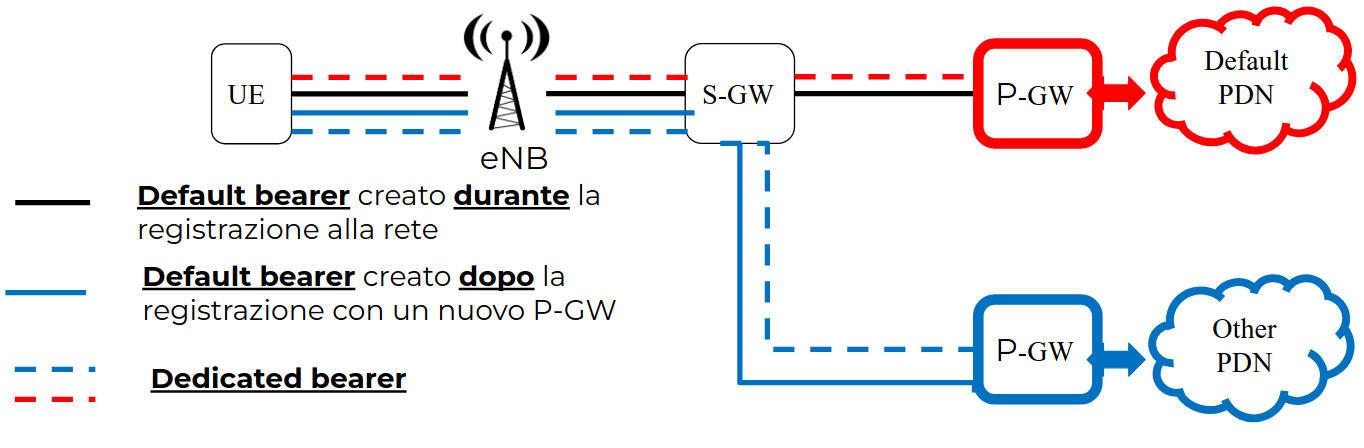
\includegraphics[width=0.9\linewidth]{img/4g/dedicatedbearing}
\end{center}
Fino ad un massimo di 8.

\paragraph{Qos e EPS Bearers:} In base al servizio si può avere uno specifico \textbf{QoS Class Identifier} (QCI), con le rispettive caratteristiche: un bit rate minimo garantito oppure no (Guaranteed Bit Rate GBR vs Non-GBR), oltre che una priorità, delay e loss rate massimo. 

I \textbf{Traffic Flow Template TFT} sono delle "mappe" istanziate al momento della connessione sul dispositivo e contengono regole generate dall'operatore telefonico per mappare un servizio sul device a una classe di QoS. Permettono di determinare la QoS che avrà un servizio (es: YouTube penso avrà QCI 7).

Tabella QCI:
\begin{center}
	\resizebox{\textwidth}{!}{\begin{tabular}{c C{1.5cm} c C{1.5cm} C{2cm} C{5cm}} 
			\toprule
			\textbf{QCI} 
			& \textbf{Resource Type} 
			& \textbf{Priority} 
			& \textbf{Packet Delay Budget (ms)} 
			& \textbf{Packet Error Loss Rate} 
			& \textbf{Example Services} \\
			\midrule
			1 & GBR     & 2 & 100 & $10^{-2}$ & Conversational voice \\
			\hline
			2 & GBR     & 4 & 150 & $10^{-3}$ & Conversational video (live streaming) \\
			\hline
			3 & GBR     & 5 & 300 & $10^{-6}$ & Non-conversational video (buffered streaming) \\
			\hline
			4 & GBR     & 3 &  50 & $10^{-3}$ & Real-time gaming \\
			\hline
			5 & Non-GBR & 1 & 100 & $10^{-6}$ & IMS signaling \\
			\hline
			6 & Non-GBR & 7 & 100 & $10^{-3}$ & Voice, video (live streaming), interactive gaming \\
			\hline
			7 & Non-GBR & 6 & 300 & $10^{-6}$ & Video (buffered streaming) \\
			\hline
			8 & Non-GBR & 8 & 300 & $10^{-6}$ & TCP-based (for example, WWW, e-mail), chat, FTP, p2p file sharing, progressive video and others \\
			\hline
			9 & Non-GBR & 9 & 300 & $10^{-6}$ &  \\
			\bottomrule
	\end{tabular}}
\end{center}

%End L18

\subsection{Procedura di Collegamento alla rete operatore}

Cosa succede quando un dispositivo spento (o almeno la radio) si accende. Quando il dispositivo UE viene acceso si trova in uno degli \textbf{stati}: 
\begin{itemize}
	\item \texttt{EMM-DEREGISTERED}: EPS Mobility Management EMM non registrato e la sua mobilità non è gestita; all'interno della rete core nessuno gestisce questo dispositivo

	\item \texttt{ECM-IDLE}: EPS Connection Management: connessione tra UE e MME per il traffico di controllo non attivo

	\item \texttt{RRC\_IDLE}: Radio Resource Control UE non è connesso a nessun eNodeB; rilascia anche tutti i canali di controllo. Questo stato è quello in cui il dispositivo si trova quando in risparmio energetico
\end{itemize}

Due \textbf{modalità di selezione} della rete: 
\begin{itemize}
	\item \textbf{automatica}: in base alla SIM, la quale contiene country code e network code

	\item \textbf{manuale}: selezionandola manualmente dall'elenco delle reti operatore presenti
\end{itemize}

Certe BS possono essere riservate a certi abbonati (femtocella): \textbf{Closed Subscriber Group CSG}. Opzionale, attivata solo in presenza di una femtocella. Viene fatto dopo la selezione della rete a cui collegarsi.

L'ultimo passaggio prima di potersi collegare alla BS è la \textbf{scelta della cella} con cui iniziare la procedura di registrazione. Il criterio di selezione si basa su diversi fattori, tra cui: 
\begin{itemize}
	\item potenza di trasmissione UE (ci arrivo alla BS?)
	
    \item potenza del segnale ricevuto
\end{itemize}

Tutto questo era ancora prima di inviare dati, UE ha solo ascoltato. Adesso Inizia la \textbf{procedura di contesa} per l'\textbf{accesso allo scheduling della cella} selezionata.

Dopo aver ottenuto l'accesso, inizia una prima fase di \textbf{configurazione livelli MAC e L1}, ovvero la configurazione dei canali radio per la trasmissione.

A questo punto il dispositivo è all'interno dello scheduling della BS ed ha una connessione alla rete core, quindi lo stato è \texttt{RRC\_CONNECTED}. Non si ha nessuna garanzia sulla procedura di allacciamento alla rete core, per ora si ha solo la connessione con una BS.

Si avvia la procedura di \textbf{collegamento tra UE e la rete core} tramite i messaggi di controllo scambiati con l'MME. Prima fase che coinvolge anche la rete core, si usano i protocolli NAS (Non Access Stratum).

A questo punto lo stato è \texttt{EMM-REGISTERED}, \texttt{ECM-CONNECTED} (se tutto è andato a buon fine).

Nel caso UE rimanga inattivo (si scollega per qualsiasi motivo), lo stato non diventa "deregistrato", ma solamente \texttt{RRC\_IDLE} (non bisogna ripetere la connessione completa, troppo lunga).

\begin{center}
	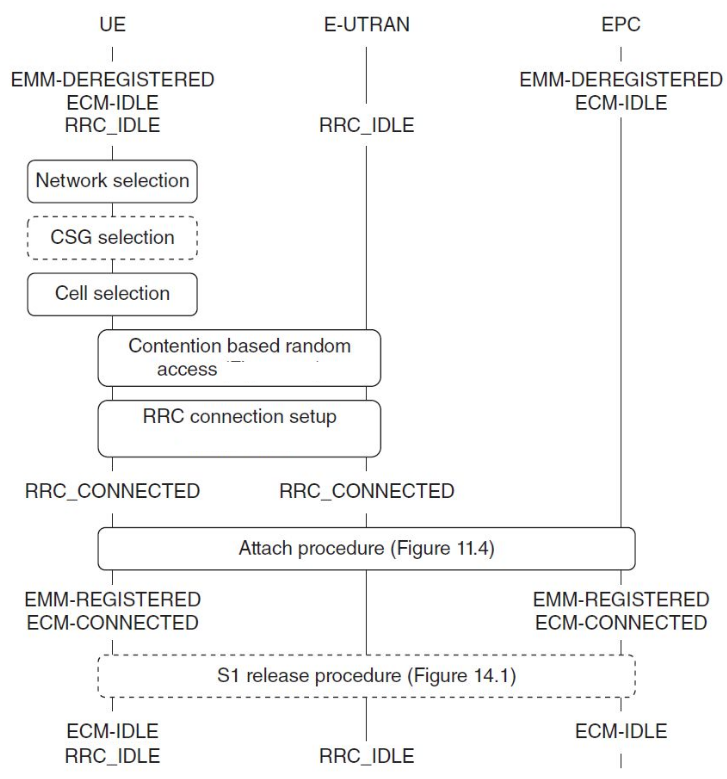
\includegraphics[width=0.75\linewidth]{img/4g/collop}
\end{center}

\subsection{Procedure di Handover}

In LTE esiste \textbf{solo hard-handover}, non c'è mai un momento in cui un UE è collegato a due BS contemporaneamente.

Si distinguono due classi di handover (sempre hard):
\begin{itemize}
	\item \textbf{Seamless handover}: minore latenza, ammette ritrasmissioni; l'obiettivo è non far percepire l'handover, viene fatto nel modo più veloce possibile. Viene usato per cose come Traffico VoIP. Suscettibile al buco di connessione, ma veloce

	\item \textbf{Lossless handover}: maggiore latenza, riduce la perdita di pacchetti. Tipicamente usato per traffico HTTP/FTP, usato quando la ritrasmissione è lenta e la si vuole eliminare il più possibile.
\end{itemize}

\paragraph{Lossless handover:} Tipicamente a livello di data link si ha affidabilità (ACK e NACK per i dati trasmessi). Si tratta di un hard handover, quindi ci sarà un momento in cui il device non è collegato a nulla (sta tentando di entrare nello scheduling della BS destinazione). 

Per evitare di perdere pacchetti in downlink durante questa fase, il flusso di download continuerà a mandare i dati alla vecchia BS (TEID ancora quello vecchio), ma le due eNodeB sanno che è in corso un handover quindi la vecchia BS inoltra tramite X2 tutti i dati di cui non è stato ancora fatto ACK alla BS destinazione, la quale li buffererà per poi inviarli alla fine della procedura di handover. 

Ci sono dei limiti, entro una certa durata di handover (e di quantità di dati) la prima BS gestisce i dati. Se la procedura dura troppo cade la linea.

\subsubsection{Handover S1}

Lo UE vuole \textbf{cambiare BS e MME}. Quindi 5 parti (UE, source e target eNodeB e MME). L'handover viene \textbf{deciso lato eNodeB}. 

Gran parte della procedura coinvolge la rete core: questo per rendere tutto il più possibile trasparente all'UE. Dato che si tratta di hard handover, il passaggio viene effettuato solo una volta che le risorse "dall'altro lato" sono pronte. 

Passaggi: 
\begin{itemize}
	\item Il primo passo è la \textbf{source eNodeB} che notifica la \textbf{richiesta di handover} all'MME che la gestisce

	\item Il \textbf{source MME} invia una \textbf{Forward Relocation Request} ("c'è da cambiare una connessione") al target MME

	\item Il \textbf{target MME} contatta il target eNodeB per notificargli la \textbf{richiesta di handover} che riguarda quella BS

	\item Poi c'è una fase di \textbf{resource setup}: la \textbf{target BS} prepara le risorse per ospitare il futuro UE

	\item La \textbf{target eNodeB} risponde al suo MME con un \textbf{handover request ACK}

	\item Il \textbf{target MME} risponde alla \textbf{relocation request} fatta dal source MME

	\item Il \textbf{source MME} a questo punto invia alla sua BS (source eNodeB) il \textbf{comando di handover}

	\item La \textbf{BS} inoltra all'UE il \textbf{comando di handover}, contenente tutte le informazioni per cambiare connessione

	\item La \textbf{source eNodeB} invia il \textbf{trasferimento dello stato} di gestione al suo MME

	\item Se lossless handover: si ha un collegamento diretto su X2 tra le eNodeB per inoltrare i dati

	\item Una volta avvenuto il trasferimento dello stato lato core, il \textbf{target MME} dice al target eNodeB le \textbf{informazioni} sul \textbf{trasferimento di stato}

	\item Lo \textbf{UE} invia la \textbf{conferma dell'handover} al target eNodeB

	\item Il \textbf{target eNodeB} conferma al suo MME che l'handover è avvenuto con successo (\textbf{handover notify})

	\item I \textbf{due MME} si scambiano un messaggio di \textbf{Forward relocation complete} e il relativo \textbf{ACK}

	\item Lo \textbf{UE} invia all'MME l'\textbf{update della tracking area}

	\item Il vecchio MME dice alla vecchia BS di \textbf{rilasciare le risorse}
\end{itemize}

\begin{center}
	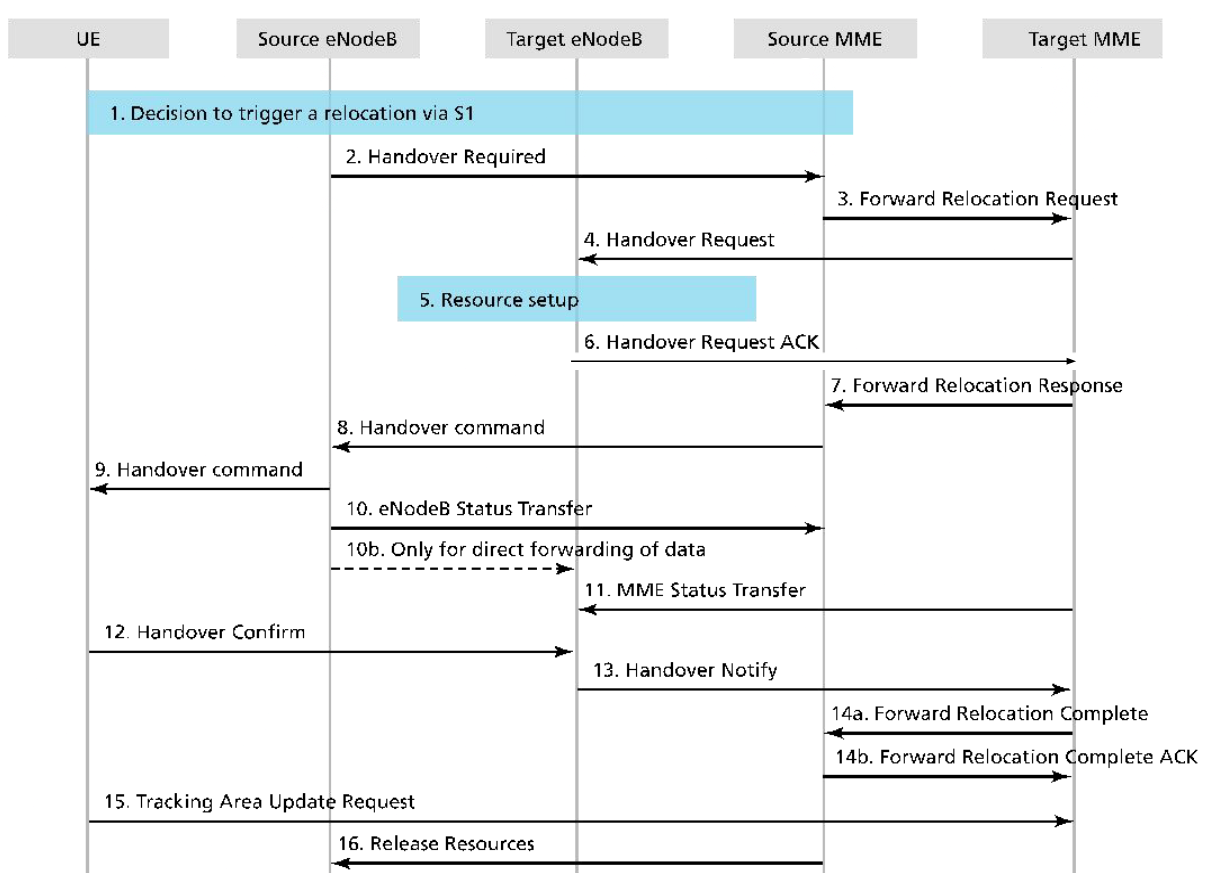
\includegraphics[width=0.98\linewidth]{img/4g/hand1}
\end{center}

Si ha una parte di \textbf{predisposizione delle risorse} sulla rete core, quando è tutto pronto viene mandato il \textbf{comando di handover}, una volta confermato l'handover l'ultima cosa è \textbf{rilasciare le risorse} originali.

\subsubsection{Handover X1}

Coinvolge meno la rete core; fatta nel caso in cui \textbf{non bisogna cambiare TA e MME}. 

Passaggi: 
\begin{itemize}
	\item Viene \textbf{deciso l'handover}

	\item La \textbf{richiesta di handover} viene mandata direttamente \textbf{tra source e target eNodeB} (tramite X2)

	\item Viene fatto il \textbf{setup delle risorse} per la \textbf{target eNodeB}

	\item Quando è tutto pronto viene mandato un \textbf{ACK} alla source eNodeB

	\item La \textbf{source eNodeB} manda il \textbf{comando di handover} allo UE

	\item \textbf{Trasferimento di stato} tra le eNodeB

	\item Messaggio da \textbf{UE} a target eNodeB di \textbf{handover completato}

	\item L'ultima cosa è una \textbf{path switch request} (e il suo \textbf{ACK}): cambio dei bearer di livello tra rete core e RAN (cambio TEID)

	\item Una volta terminata la path switch il nuovo eNodeB dice alla source eNodeB di \textbf{lasciare le risorse}
\end{itemize}

\begin{center}
	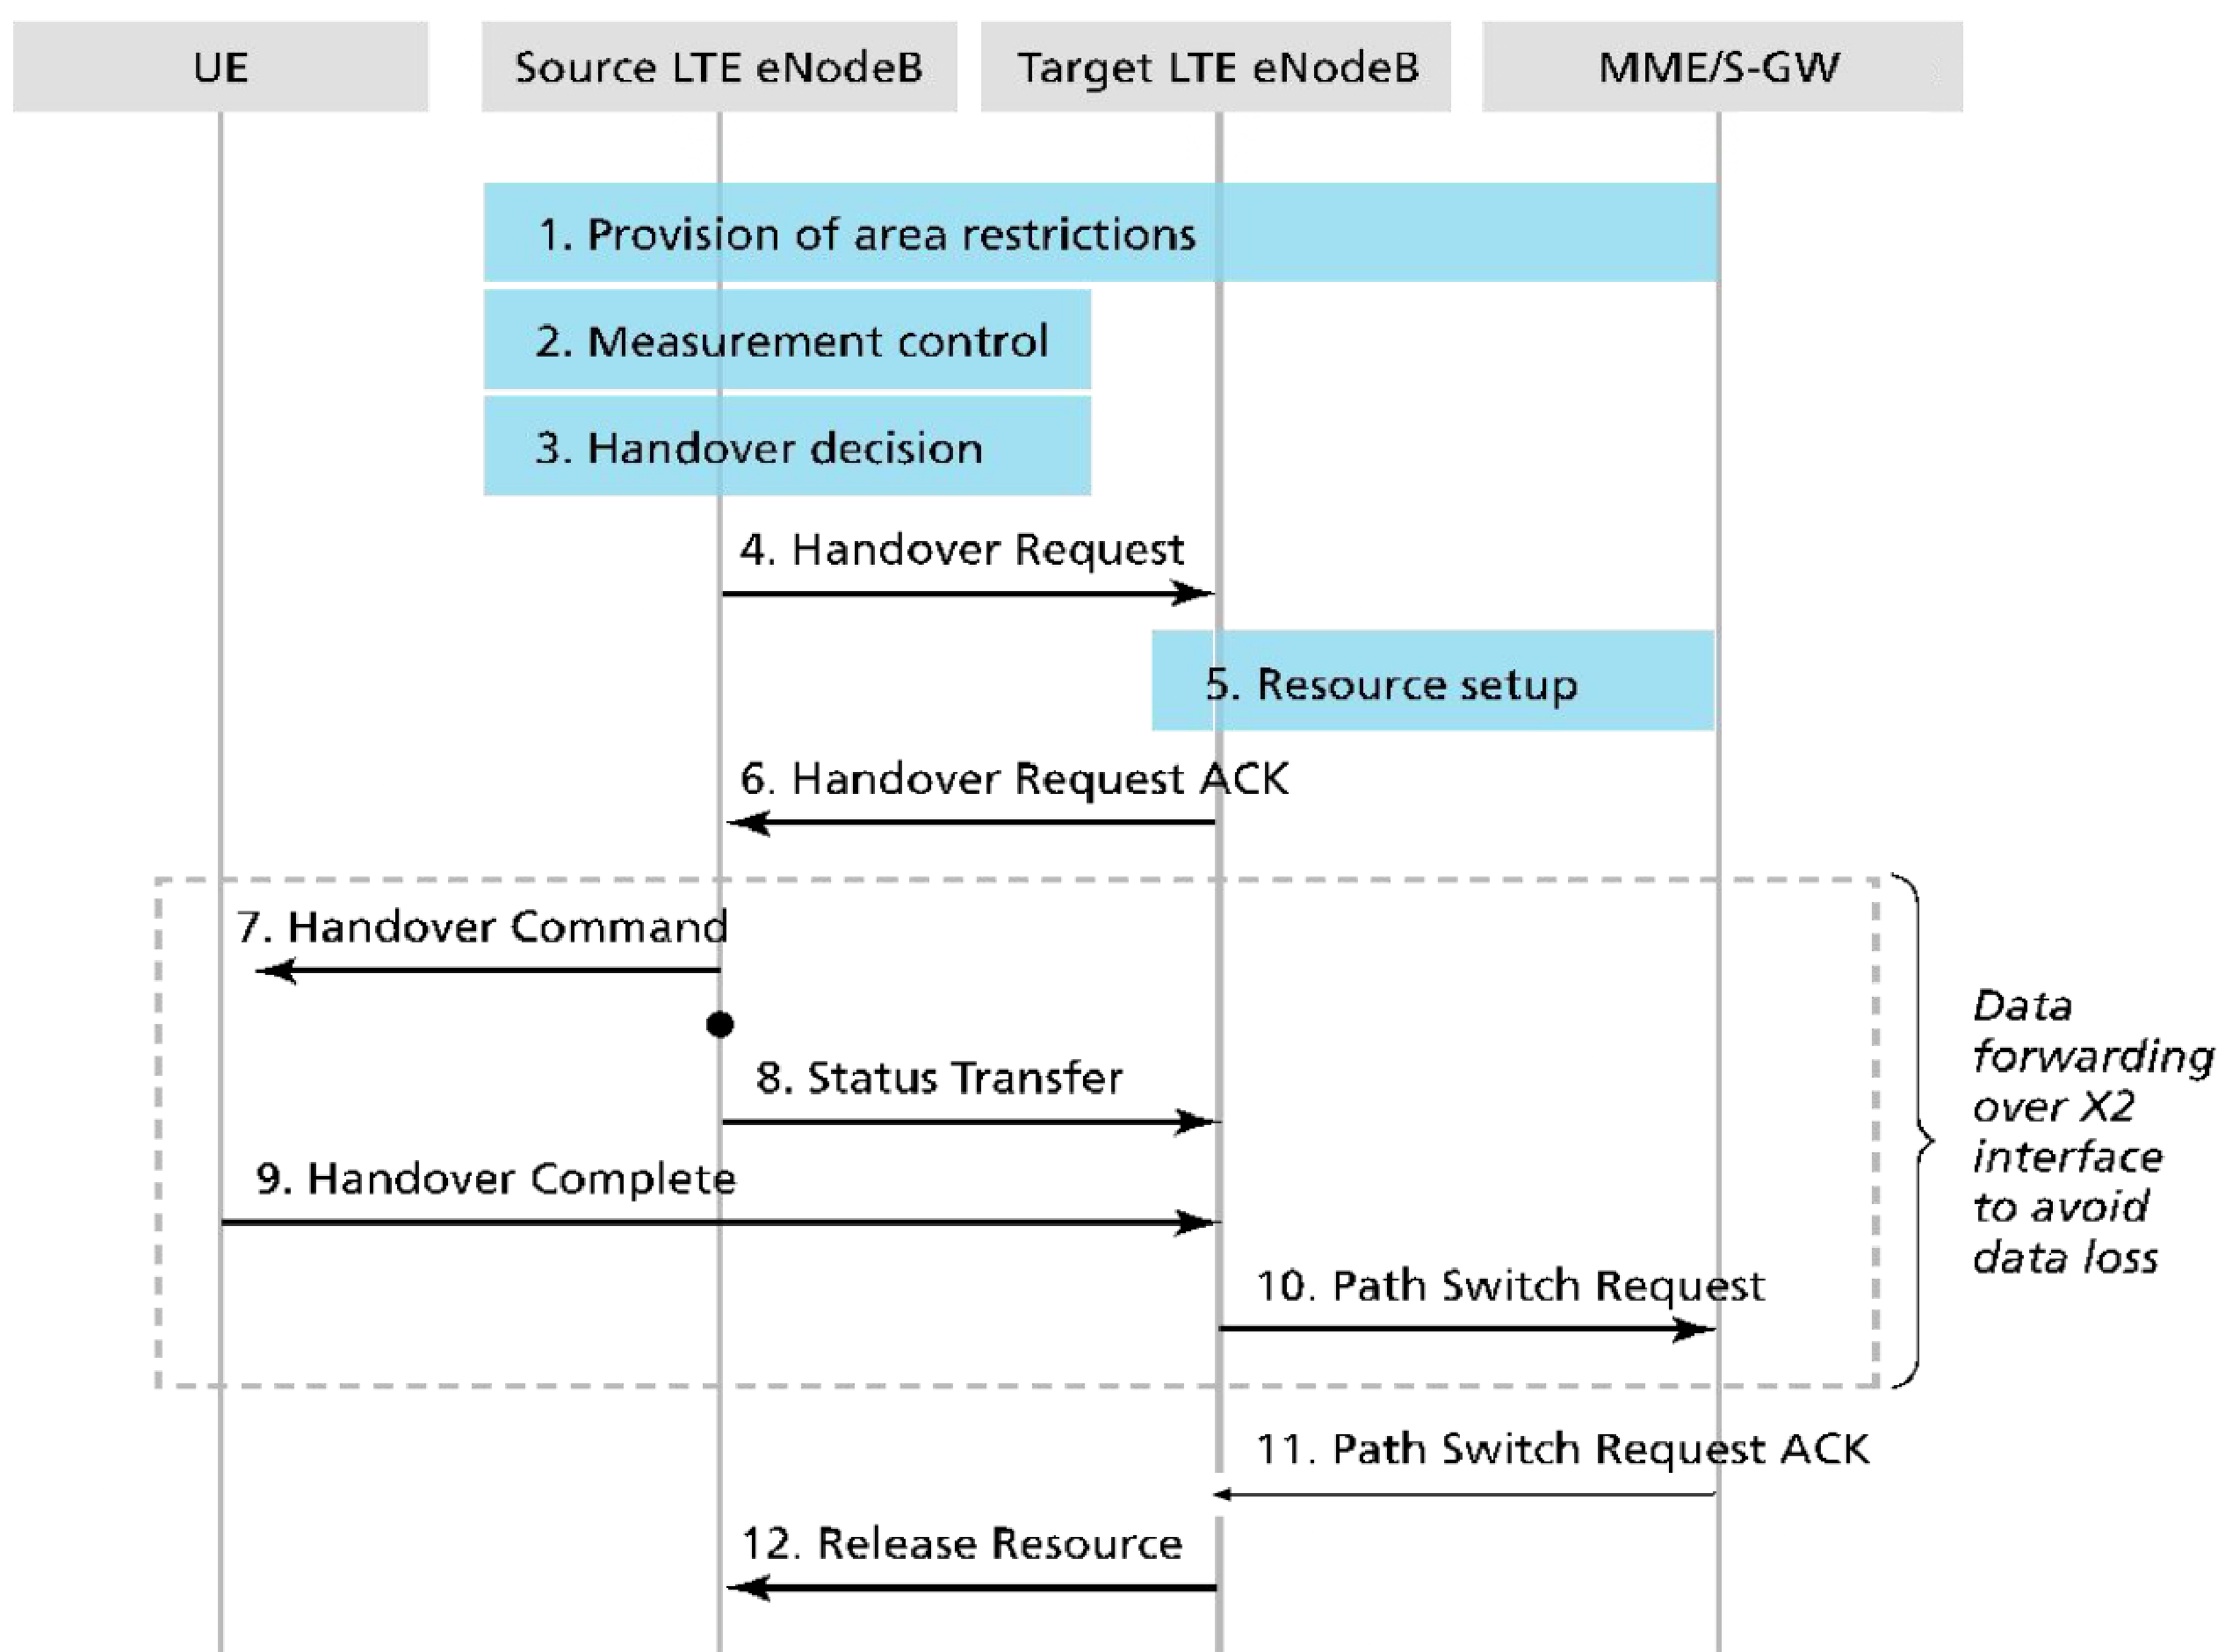
\includegraphics[width=0.94\linewidth]{img/4g/hand2}
\end{center}

La procedura è sempre simile: preparazione risorse, comando di handover, se tutto è andato bene rilascio delle risorse originali.
    
    % !TeX spellcheck = it_IT
\section{5G}

Vengono aggiunti \textit{sempre più casi d'uso diversi tra loro}, e quindi il relativo supporto. Ci sono diversi casi d'uso completamente differenti, come ad esempio:
\begin{itemize}
	\item Multi-hop communication: comunicazione a più salti tra dispositivi per estendere la copertura e migliorare la connettività, utile in ambienti urbani o in aree remote
	\item Device-to-device communication and cooperative devices: comunicazione diretta tra dispositivi senza passare dalla rete centrale, per aumentare efficienza e ridurre la latenza	
	\item Ultra-reliable communication: comunicazioni ad altissima affidabilità, ad esempio per infrastrutture critiche come reti elettriche o trasporti
	\item Massive machine communication: connessione simultanea di un gran numero di dispositivi IoT, tipico di fabbriche smart, logistica e sensori ambientali	
	\item Inter-vehicular/vehicular-to-road communication: comunicazioni tra veicoli e tra veicoli e infrastrutture stradali per supportare la guida autonoma e la sicurezza stradale
	\item Ultra-dense deployments: aree con altissima densità di dispositivi connessi, come uffici o stadi, dove il 5G garantisce prestazioni elevate nonostante l'affollamento.
\end{itemize}
Si ampia il range di frequenze: va da $300MHz$ a $300GHz$. Comprende diverse fasce di frequenza.\\

\newpage

\paragraph{Classificazione International Telecommunication Unit ITU:} Secondo l'ITU le applicazioni possono essere classificate in tre principali categorie di utilizzo:
\begin{itemize}
	\item \textbf{Enhanced Mobile Broadband (eMBB)}
	\begin{itemize}
		\item Servizi orientati alle persone
		\item Elevata banda
		\item HD Streaming, AR/VR
	\end{itemize}
	\item \textbf{Ultra-reliable and Low-latency communication (uRLLC)}
	\begin{itemize}
		\item Servizi orientate alle industrie
		\item Bassissima latenza e affidabilità
		\item Controllo remoto, guida autonoma
	\end{itemize}
	\item \textbf{Massive Machine Type Communications (mMTC)}
	\begin{itemize}
		\item alta densità di connessioni (anche con bassa quantità di dati trasmessi)
		\item smart cities/smart agriculture
	\end{itemize}
\end{itemize}

\begin{center}
	\resizebox{\linewidth}{!}{\renewcommand{\arraystretch}{1.2}
		\begin{tabular}{l | l}
			\textbf{Key Performance Indicator KPI} & \textbf{Minimum Performance Requirement} \\
			\hline
			\multirow{2}{*}{Peak Data Rate} & Downlink: 20 Gbps \\
			\cline{2-2}
			& Uplink: 10 Gbps \\
			
			\hline 
			\multirow{2}{*}{Peak Spectral Efficiency} & Downlink: 30 bps/Hz \\
			\cline{2-2}
			& Uplink: 15 bps/Hz \\
			\hline
			
			\multirow{2}{*}{User-Experienced Rate} & Downlink: 100 Mbps \\
			\cline{2-2}
			& Uplink: 50 Mbps \\
			\hline
			
			5th-Percentile User & Downlink: 0.12 bps/Hz $\approx$ 0.3 bps/Hz \\
			\cline{2-2}
			Spectral Efficiency & Uplink: 0.045 bps/Hz $\approx$ 0.21 bps/Hz \\
			\hline
			
			\multirow{2}{*}{Average Spectral Efficiency} & Downlink: 3.3 bps/Hz $\approx$ 9 bps/Hz \\
			\cline{2-2}
			& Uplink: 1.6 bps/Hz $\approx$ 6.75 bps/Hz \\
			\hline
			
			Area Traffic Capacity & 10 Mbps/m$^2$ (Indoor Hotspot) \\
			\hline
			
			\multirow{2}{*}{User Plane Latency} & 4ms - eMBB \\
			\cline{2-2}
			& 1ms - URLLC \\
			\hline
			
			Control Plane Latency & 20ms \\
			\hline
			
			Connection Density & 1'000'000 devices per km$^2$ \\
			\hline
			
			\multirow{3}{*}{Energy Efficiency} & The support for two aspects: \\
			\cline{2-2}
			& (1) Efficient data transmission in a loaded case \\
			\cline{2-2} 
			& (2) Low energy consumption when there are no data \\
			\hline
			
			Reliability & $1-10^{-5}$ ($99.999\%$) \\
			\hline
			
			Mobility & Up to 500km/h \\
			\hline
			
			Mobility Interruption Time & 0ms \\
			\hline
			
			\multirow{2}{*}{Maximal Bandwidth} & 100 MHz for sub-6 GHz \\
			\cline{2-2}
			& 1 GHz for mmWave \\
			\hline
	\end{tabular}}
\end{center}

Le "direzioni" dell'evoluzione per 5G sono: 
\begin{itemize}
	\item Maggiore spettro
	\item Maggiore efficienza spettrale
	\item Riuso spaziale
	\item "Softwarizzazione" della rete
\end{itemize}

%End L19

\newpage

\subsection{Software Defined Networking SDN}

La struttura di un'applicazione di rete "normale" (senza SDN), consiste di un layer per control e data assieme, il quale si occupa sia del flusso di controllo che del flusso di dati. I dispositivi nella rete hanno al loro interno gli algoritmi di controllo e le regole di forward. \\

SDN "toglie" dai dispositivi di rete la \textbf{parte di controllo}, la quale viene \textbf{centralizzata} in un SDN controller, collegato con tutti i dispositivi e implementa le regole di controllo. Tutte le regole di controllo sono implementati ad un \textbf{livello software} al di sopra del data layer. Offre un'interfaccia unificata all'esterno della rete e permette una conoscenza topologica globale della rete stessa.\\

\begin{center}
	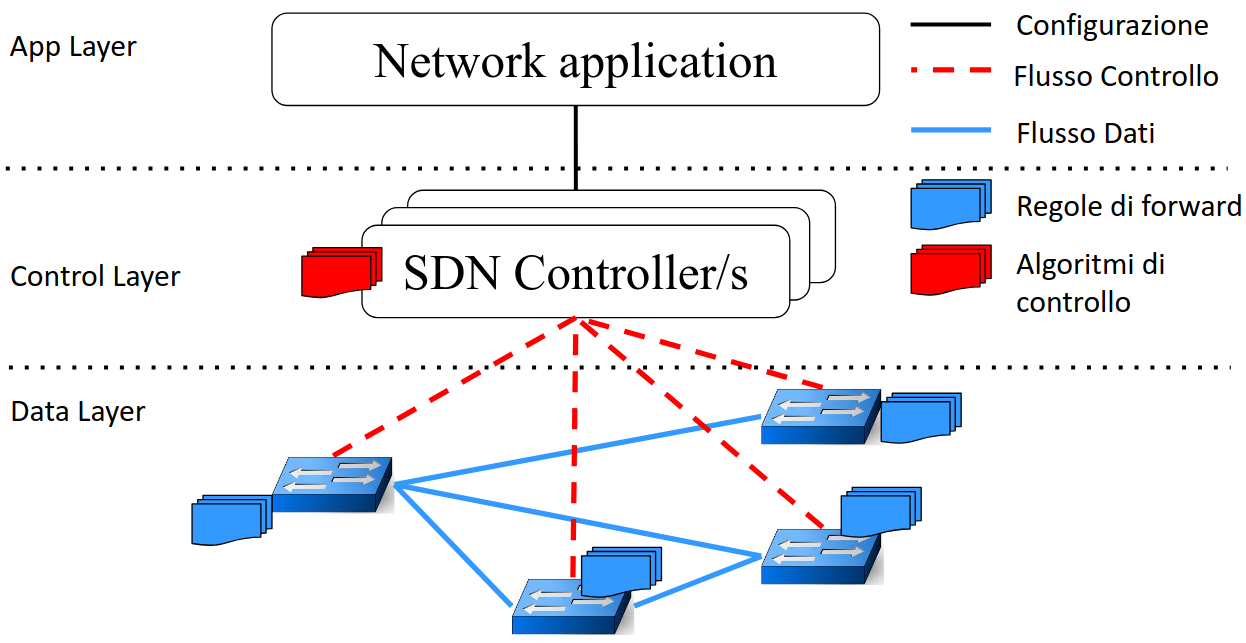
\includegraphics[width=0.8\linewidth]{img/5g/sdn1}
\end{center}

I dispositivi di rete usano un linguaggio in grado di comunicare con l'SDN controller; si ha un linguaggio apposito per la comunicazione tra controller e switch.\\
Si può lavorare anche in maniera reattiva: una volta ricevuto un pacchetto, il dispositivo richiede al controller la regola relativa. In questo modo il controller può inviare/gestire la regola anche per gli altri dispositivi presenti all'interno della rete.\\

Nel networking tradizionale, una volta definiti control e data plane non si possono più modificare i layer, con SDN e fixed-function data plane si possono modificare le funzionalità di controllo a livello software. \\

L'evoluzione vuole andare verso SDN con data plane programmabile, si ha SDN in cui tutto è programmabile, ovvero anche il livello dati ha funzionalità programmabili.
\begin{center}
	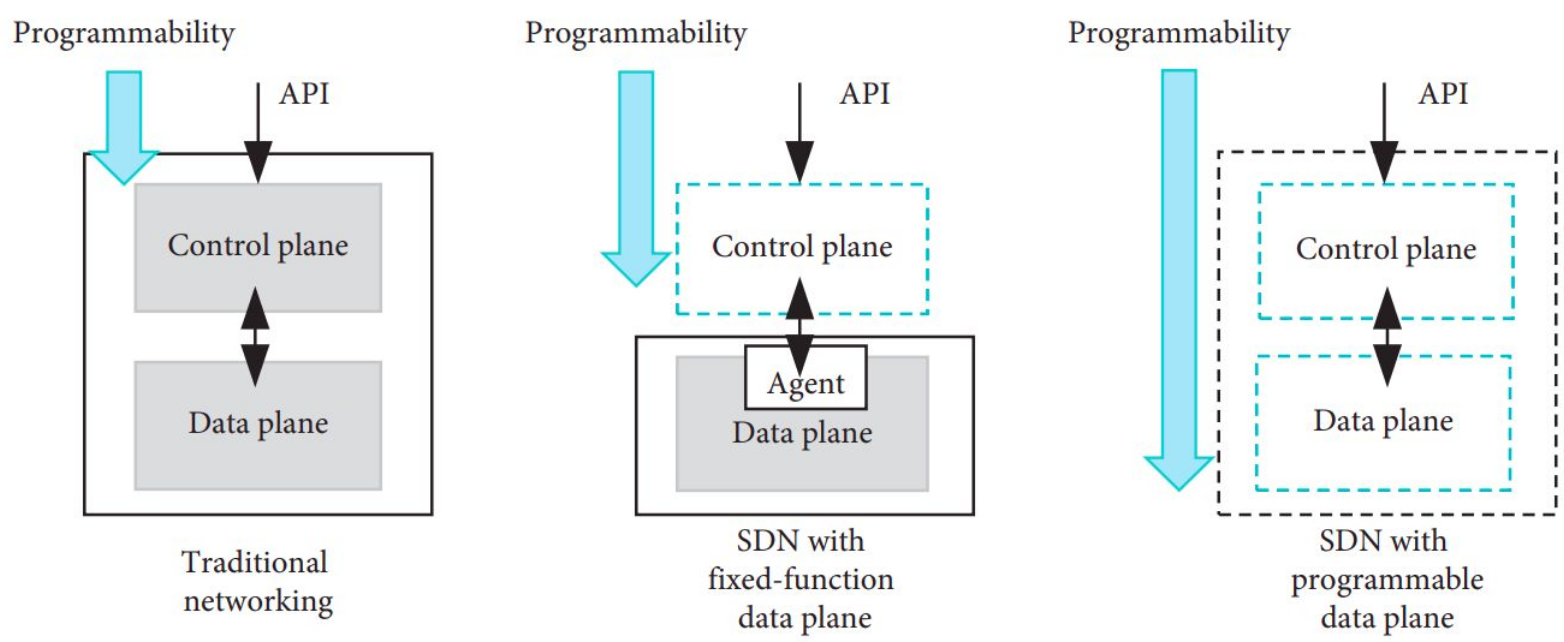
\includegraphics[width=0.85\linewidth]{img/5g/sdn2}
\end{center}
L'architettura prevede una parte di parsing programmabile: si può programmare come il pacchetto ricevuto viene processato. Se data plane è fisso, si possono programmare che regole utilizzare, ma queste devono essere implementate dal data plane, altrimenti nulla. Questo permette molta più flessibilità; le reti cambiano molto velocemente e questo permette di adattare i meccanismi alle condizioni della rete on-the-fly. Si vuole far arrivare il software fino al data link, al bordo del livello fisico.\\

I vantaggi sono diversi:
\begin{itemize}
	\item flessibilità nella gestione della rete
	\item visione centralizzata, quindi ottimizzazione del routing
	\item semplificazione della gestione a livello applicativo (OSS/BSS)
	\item testing e configurazione di nuovi protocolli di rete più semplice e veloce
\end{itemize}

Ma ci sono anche delle sfide: 
\begin{itemize}
	\item i controller diventano un single point of failure
	\item permette di reagire real-time: ma questo deve essere fatto in modo efficiente
	\item ottimizzazione del numero di regole: gestione ottimizzata delle tabelle di forwarding, gestione e garanzia dell'isolamento di reti di overlay (reti logiche), gestione della complessità
	\item sicurezza: controllare il controller vuol dire controllare la rete
\end{itemize}

\newpage

\subsection{Network Function Virtualization NFV}
Prima dell'avvento di questa tecnologia, tutto necessitava hardware dedicato; ogni componente aveva la sua soluzione hardware specifica e la soluzione software corrispondente è strettamente legata.\\

Con NFV si separano le funzionalità hardware e software. Si ha un hardware "standard" sui cui installare l'implementazione software delle funzionalità di rete richieste. Si virtualizza la parte software della funzionalità di rete per poi istanziarla a bordo di hardware standard. Si possono avere istanze in base a dove e quanto necessario.\\ 

Ma come si implementano le funzionalità di rete che implementano il servizio? \textbf{Service Function Chain (SFC)}: grafo delle funzionalità necessarie. \\
Il \textbf{NFV Orchestrator} contiene dei template per delle funzionalità e le istanzia secondo la configurazione necessaria (ovvero in base alla SFC). Si occupa anche di dove metterle (resource allocation); decide dove mettere le istanze necessarie sulle risorse hardware dedicate, in modo che rispettino tutti i vincoli: capacità dei nodi, passaggio, performance, ecc.\\

\subsubsection{Architettura NFV}

Standardizzato da ETSI. La base sono risorse hardware e tramite virtualizzazione vengono offerte risorse virtualizzate. Tutto questo diventa una NFV Infrastructure, ovvero l'infrastruttura su cui instanziare le risorse di rete virtualizzate.\\

Sulla base di questo vengono montate le \textbf{Virtual Network Functions}. Per ogni istanza viene tenuta traccia del suo stato di funzionamento: \textbf{Element Management System (EMS)}.\\

Il tutto si interfaccia alla rete operatore (BSS/OSS) tramite \textbf{NFV MANO} (Management and Orchestration). All'interno della NFV MANO si trovano
\begin{itemize}
	\item \textbf{Virtual Infrstructure Manager (VIM)}: definisce quali risorse sono disponibili e dove
	\item \textbf{VNF Manager (VNFM)}: gestisce le funzionalità di rete istanziate, presenti e future. Collegato al VIM per dire effettivamente \textit{cosa fare}, poi sarà lui che procederà all'istanziazione
	\item \textbf{Orchestrator}: coordina VNFM e VIM. Inoltre è collegato alla rete operatore per ricevere ed orchestrare le richieste all'interno della rete
\end{itemize}

I \textbf{descrittori} sono modelli per i contratti tra le varie componenti del NFV MANO, metadati strutturati che permettono all'orchestrator, VNFM e VIM di sapere cosa fare e come.

\begin{center}
	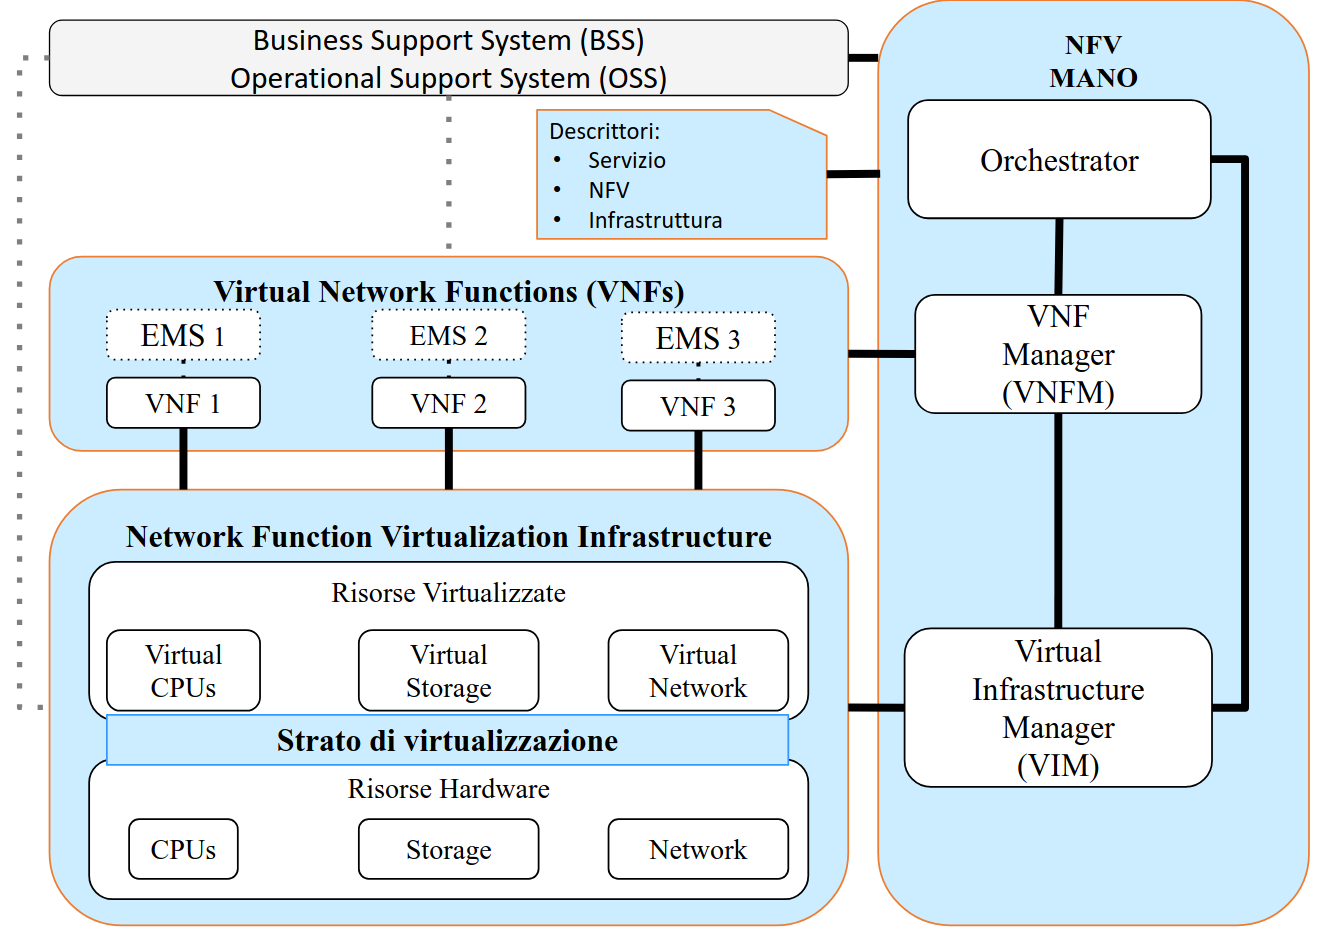
\includegraphics[width=0.8\linewidth]{img/5g/nfv1}
\end{center}

Vantaggi di NFV: 
\begin{itemize}
	\item flessibilità, scalabilità, agilità delle rete e dei servizi; intrinseco nella virtualizzazione
	\item indipendenza hardware e software; si possono modificare senza cambiare l'altro, ad esempio: fixare un bug senza cambiare l'hardware
	\item rapida prototipizzazione e introduzione di nuovi servizi, operatori ed utenti finali
	\item uso delle risorse ottimizzato e condiviso
\end{itemize}

\newpage

Sfide: 
\begin{itemize}
	\item le prestazioni devono essere comparabili con l'hardware dedicato, bisogna garantire certe prestazioni, nonostante l'overhead di virtualizzazione; esistono degli acceleratori, si vuole migliorare il più possibile le VFN, si vogliono usare migliori tecniche di virtualizzazione come Linux Container
	\item gestione efficiente delle risorse: servono tecniche ad hoc per ogni caso d'uso
	\item più software è presente, più problemi di sicurezza possibili esistono
	\item gestione della fase di transizione: devono coesistere hardware e software network function (non possiamo soppiantare la rete istantaneamente)
	\item gestione multi-tenant: più operatori di servizio possono condividere risorse hardware
\end{itemize}

\subsection*{Cloud + NFV + SDN}

5G usa tecnologie Cloud, SDN e NFV.\\

Partendo da un data center (molto) distribuito, si aggiungono le NFV sui vari componenti della rete ed i collegamenti tra questi vengono gestiti tramite SDN controller.\\

\newpage

\subsection{Centralized-RAN C-RAN e Virtual-RAN V-RAN}

La attuale architettura eNodeB è composta da Remote Radio Head RRH e Baseband Unit BBU, questo richiede: 
\begin{itemize}
	\item alimentazione
	\item condizionamento
	\item alto carico computazionale sulla BBU
	\item coordinamento via X2 per ridurre interferenze
	\item limitata visione dello stato degli altri eNodeB
	\item un singolo standard: solo 4G
\end{itemize}

Si può densificare questa struttura? Per ogni antenna bisogna inserire tutte le componenti specificate. Per risolvere questo problema si separano quindi la RRH dai livelli superiori (MAC in su), ponendoli in remoto (ma non troppo remoto, comunque c'è un vincolo geografico, 1km max circa). Si usano delle Virtual Baseband Unit, con sopra tutte le tecnologie necessarie, permettendo anche una migliore gestione in base al carico (virtualizzato).\\

Questo permette:
\begin{itemize}
	\item riduzione CAPEX (capital expenditure): si riduce il numero di apparati e si può riusare il sito, anche per introdurre nuove tecnologie RAT
	\item riduzione OPEX (operational expenditure): minor consumo energetico, ottimizzazione delle risorse BBU remote, gestione dinamica della potenza delle celle
	\item migliori prestazioni: migliore gestione delle interferenze, densificazione delle celle in maniera più sostenibile (dal punto di vista dell'operatore mobile)
	\item Multi-RAT, più tecnologie assieme (in una sola vBBU 3G, 4G e 5G)
\end{itemize}
\begin{center}
	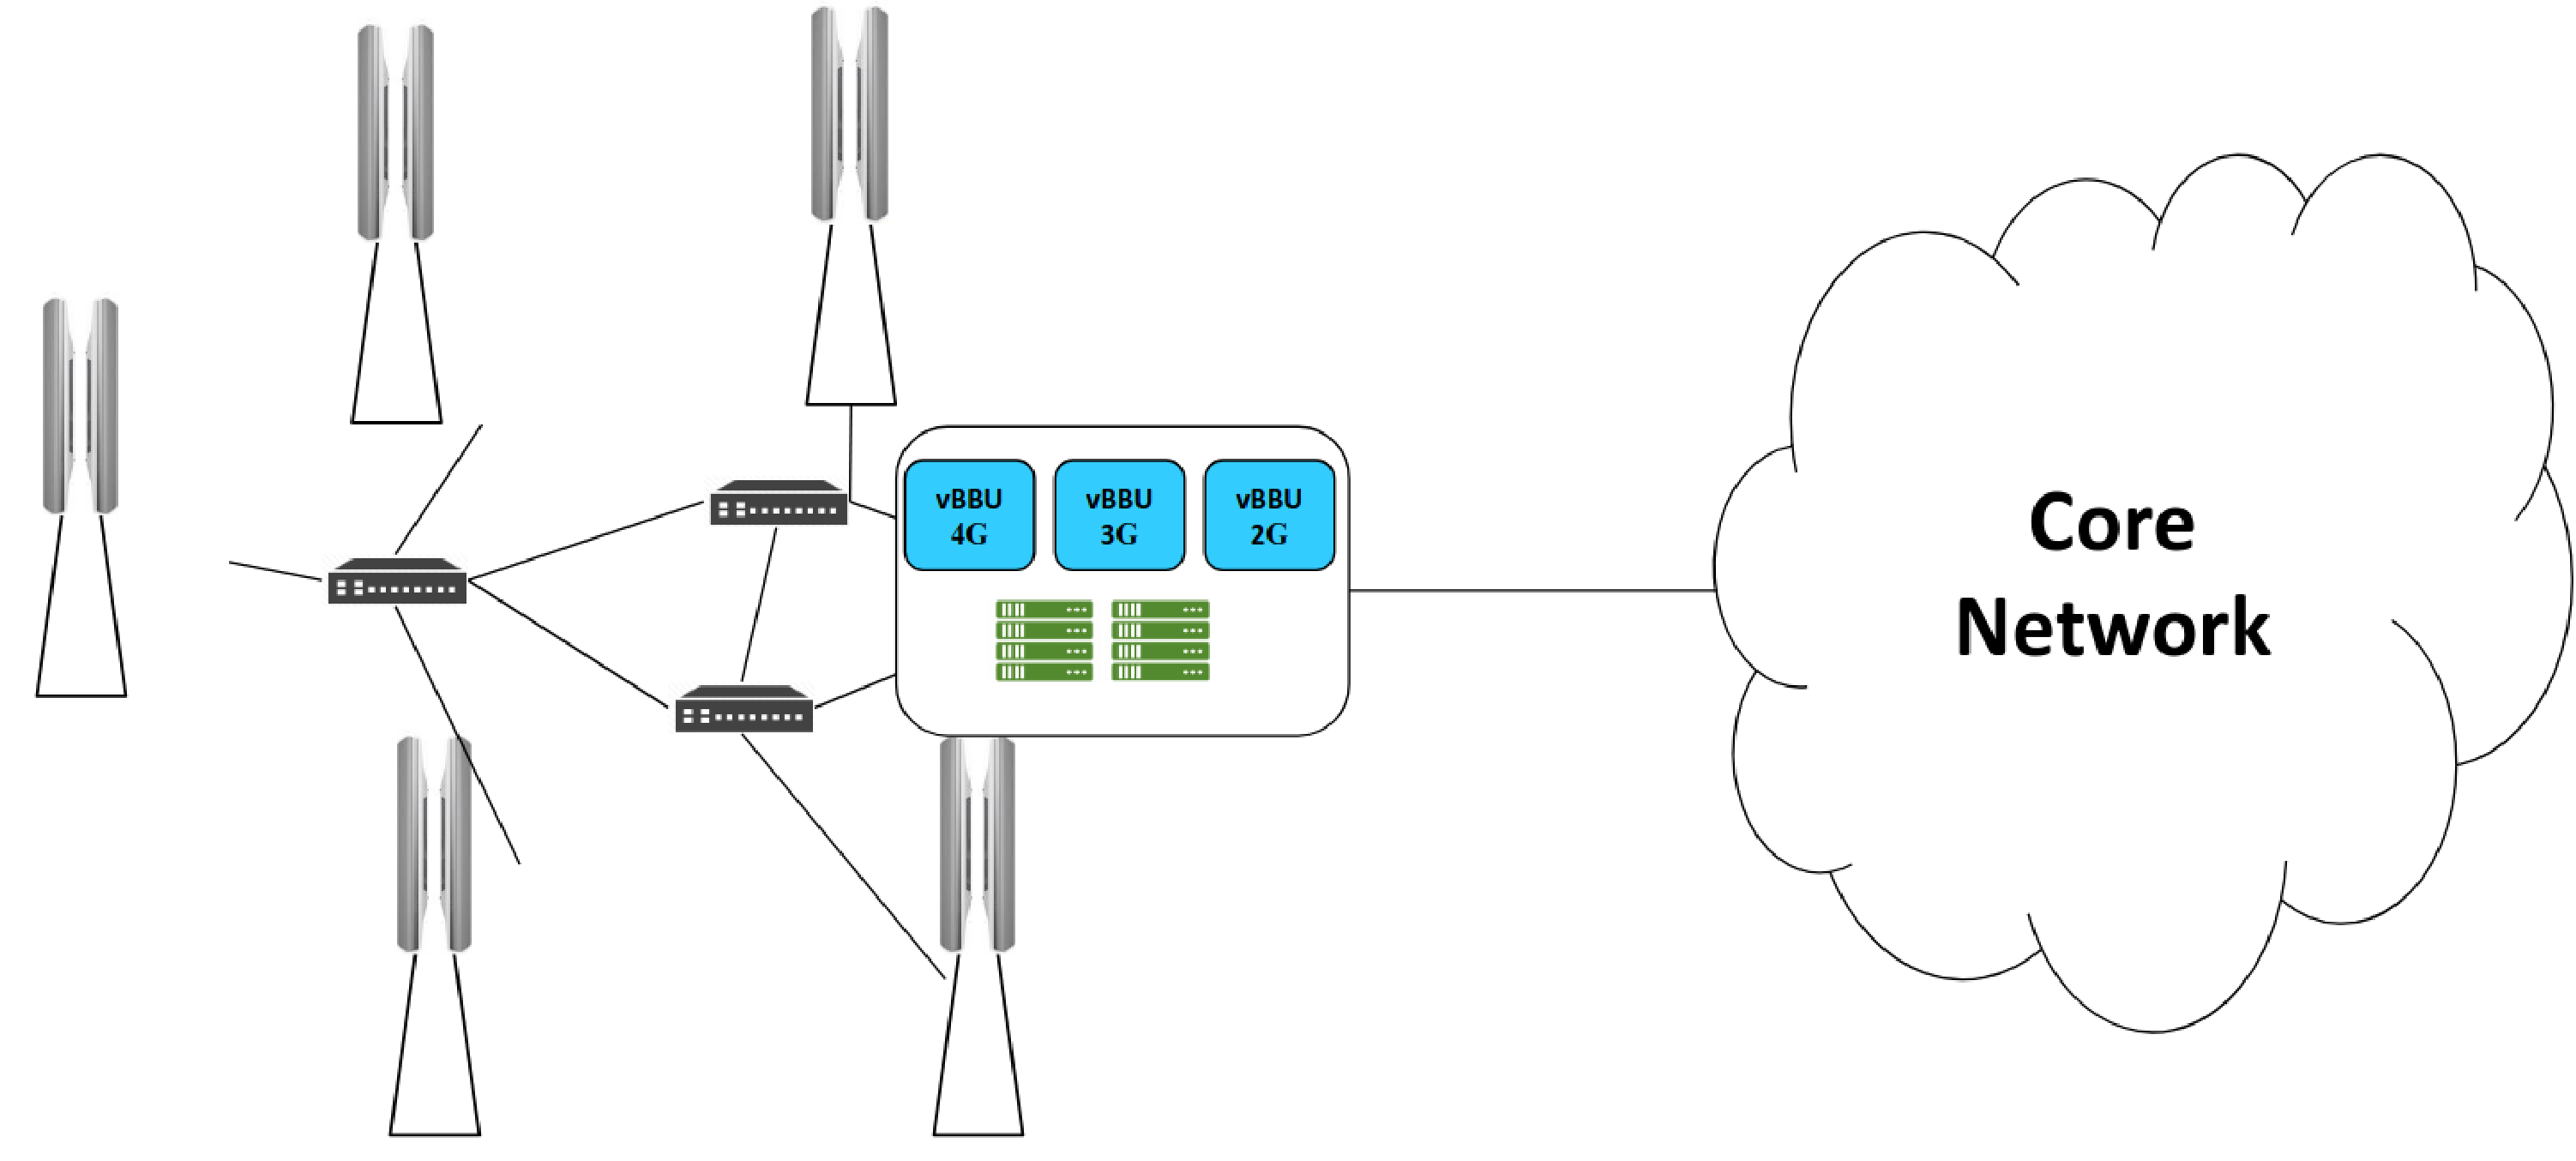
\includegraphics[width=0.98\linewidth]{img/5g/vbbu}
\end{center}

Per scalare la rete: si possono installare nuove RRH, senza dover aggiungere BBU, al posto della quale è necessario solo scalare orizzontalmente la vBBU già esistente (permetterne più istanze in parallelo, i.e., aumentare le performance). Tramite un singolo data center si possono gestire molte BS, risultando in una migliore gestione.\\

\subsection*{Cloud Computing}
Dai, sai come funziona, \href{https://it.wikipedia.org/wiki/Cloud_computing}{\texttt{ma nel caso}}. Una struttura tipica:
\begin{center}
	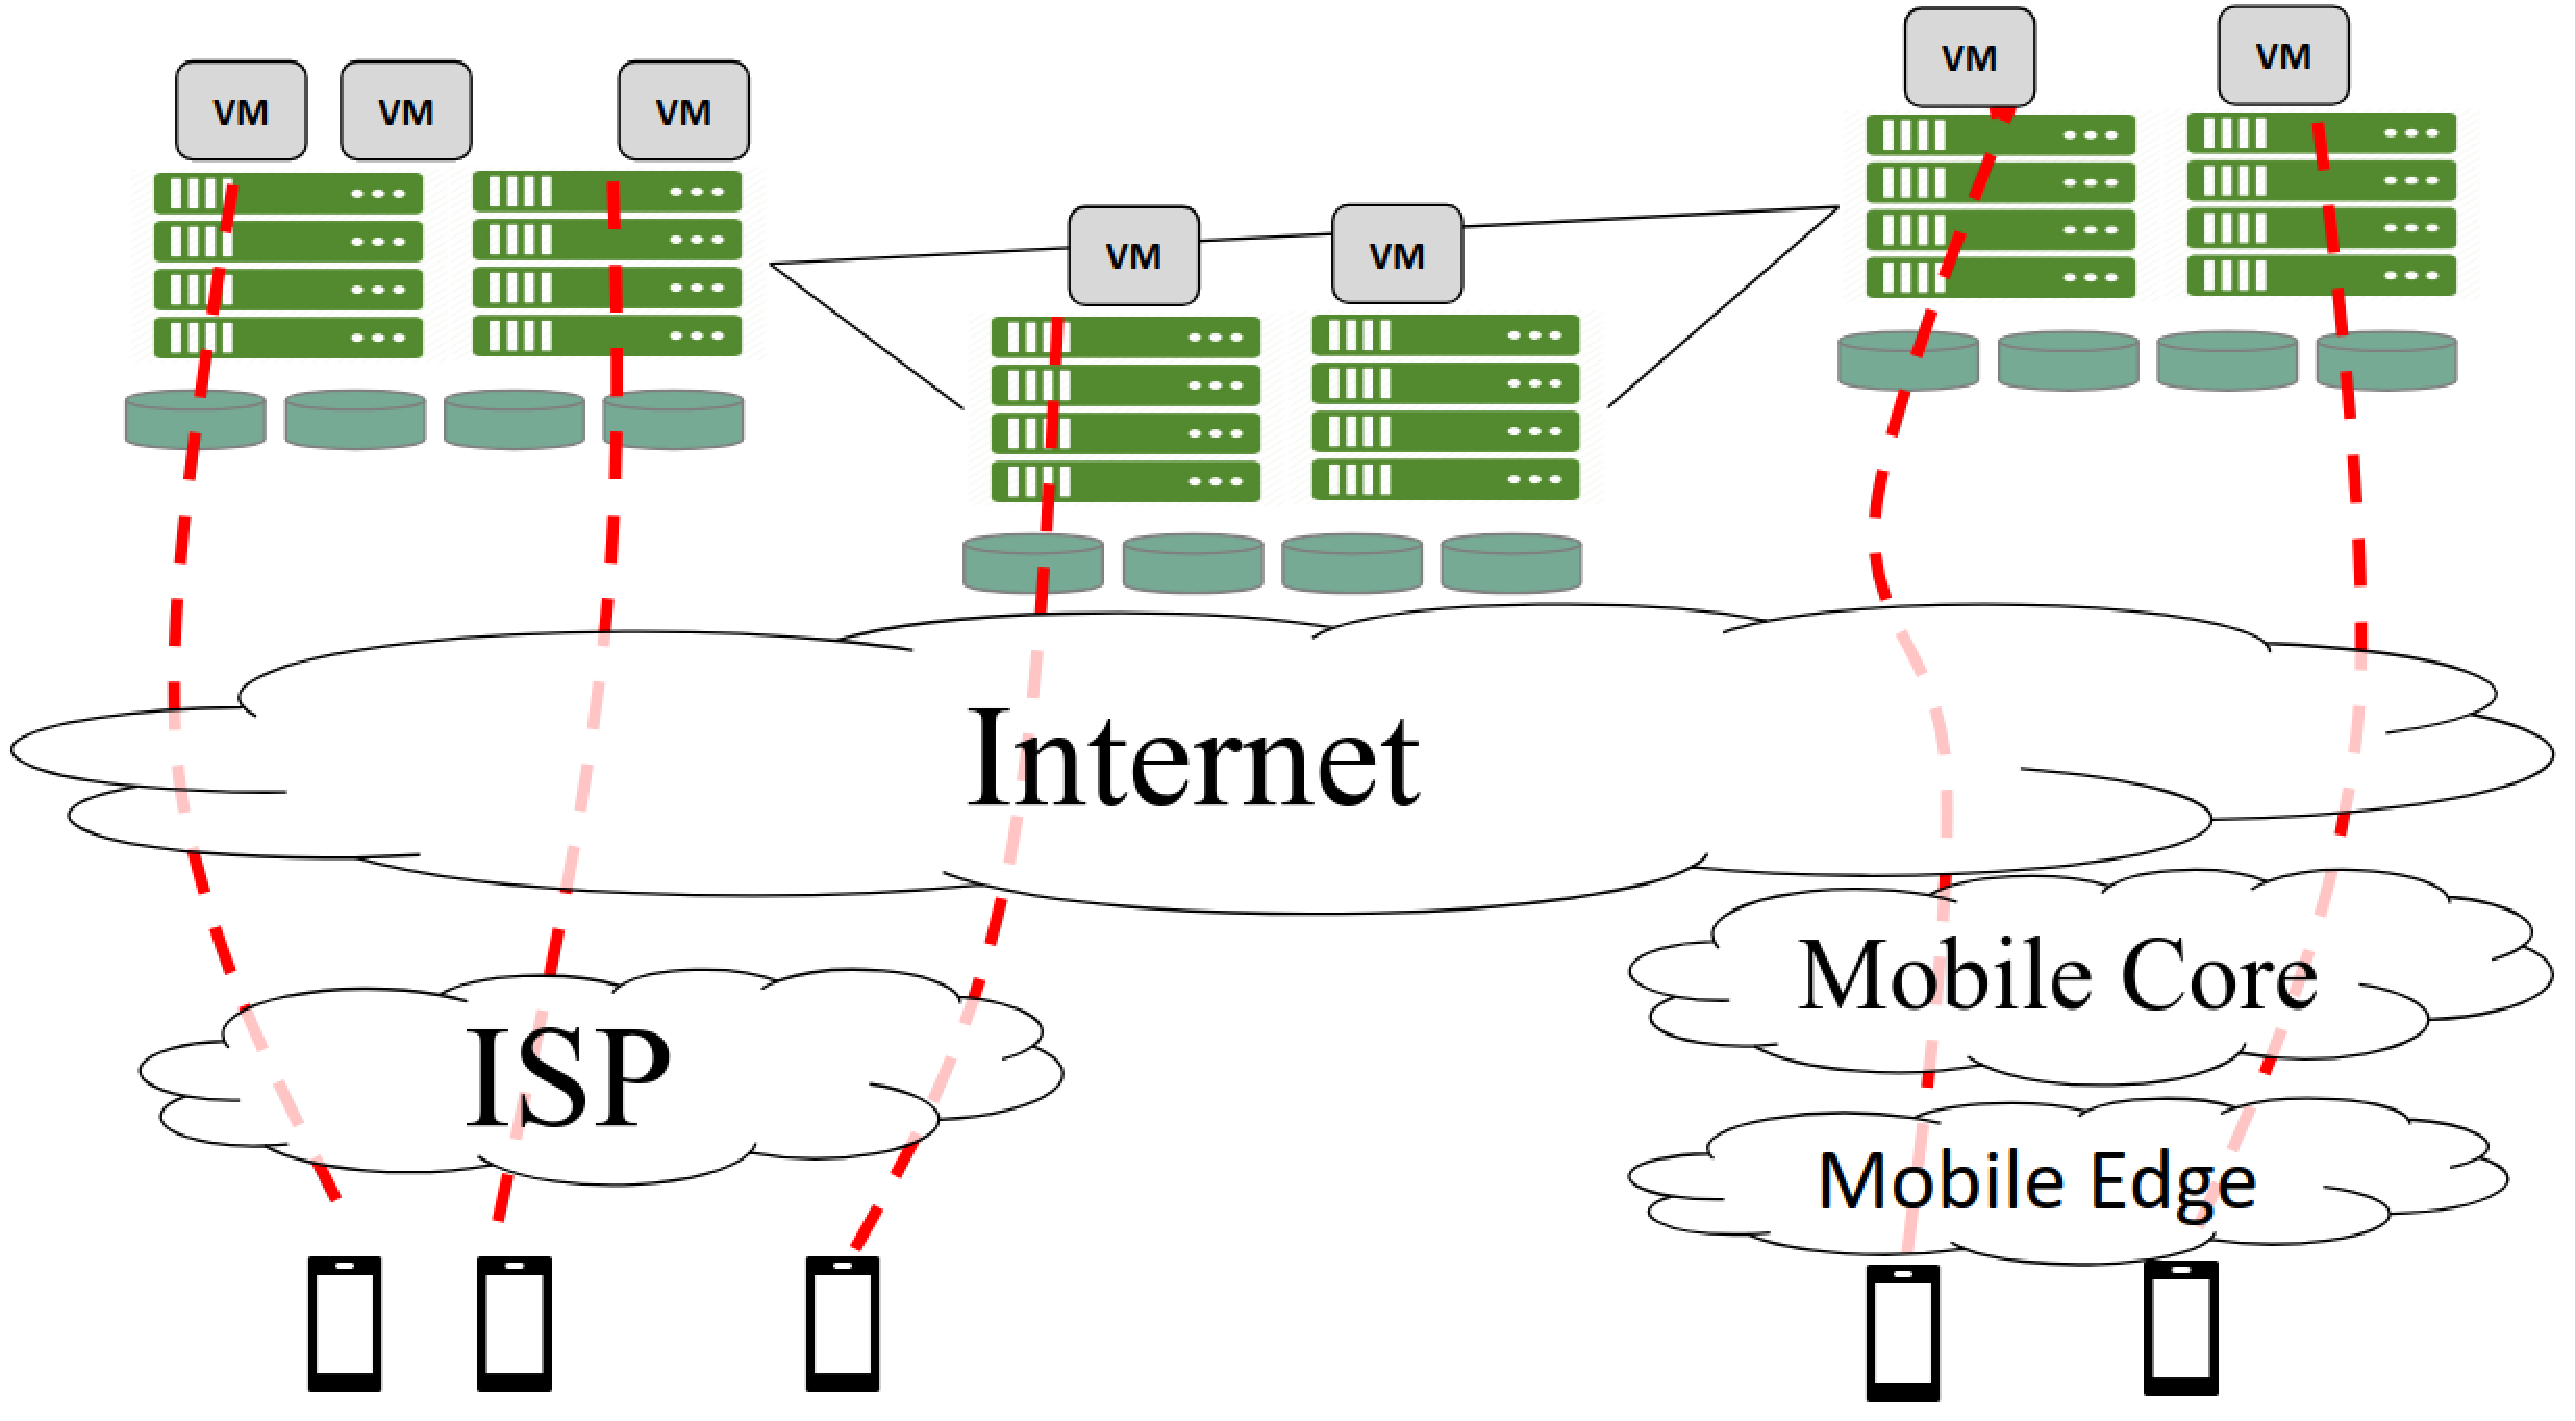
\includegraphics[width=0.8\linewidth]{img/5g/clud}
\end{center}
Questo potrebbe avere (relativamente) elevata latenza per i servizi, elevato jitter (deviazione standard sul delay alta), applicazioni near real-time sono difficili da realizzare.

\newpage

\subsection{Mobile Edge Computing MEC (ETSI)}

Mobile Edge Computing (chiamato anche Multi-access Edge Computing). Si vuole avere delle risorse computazionali il più vicino possibile all'utente. 
\begin{center}
	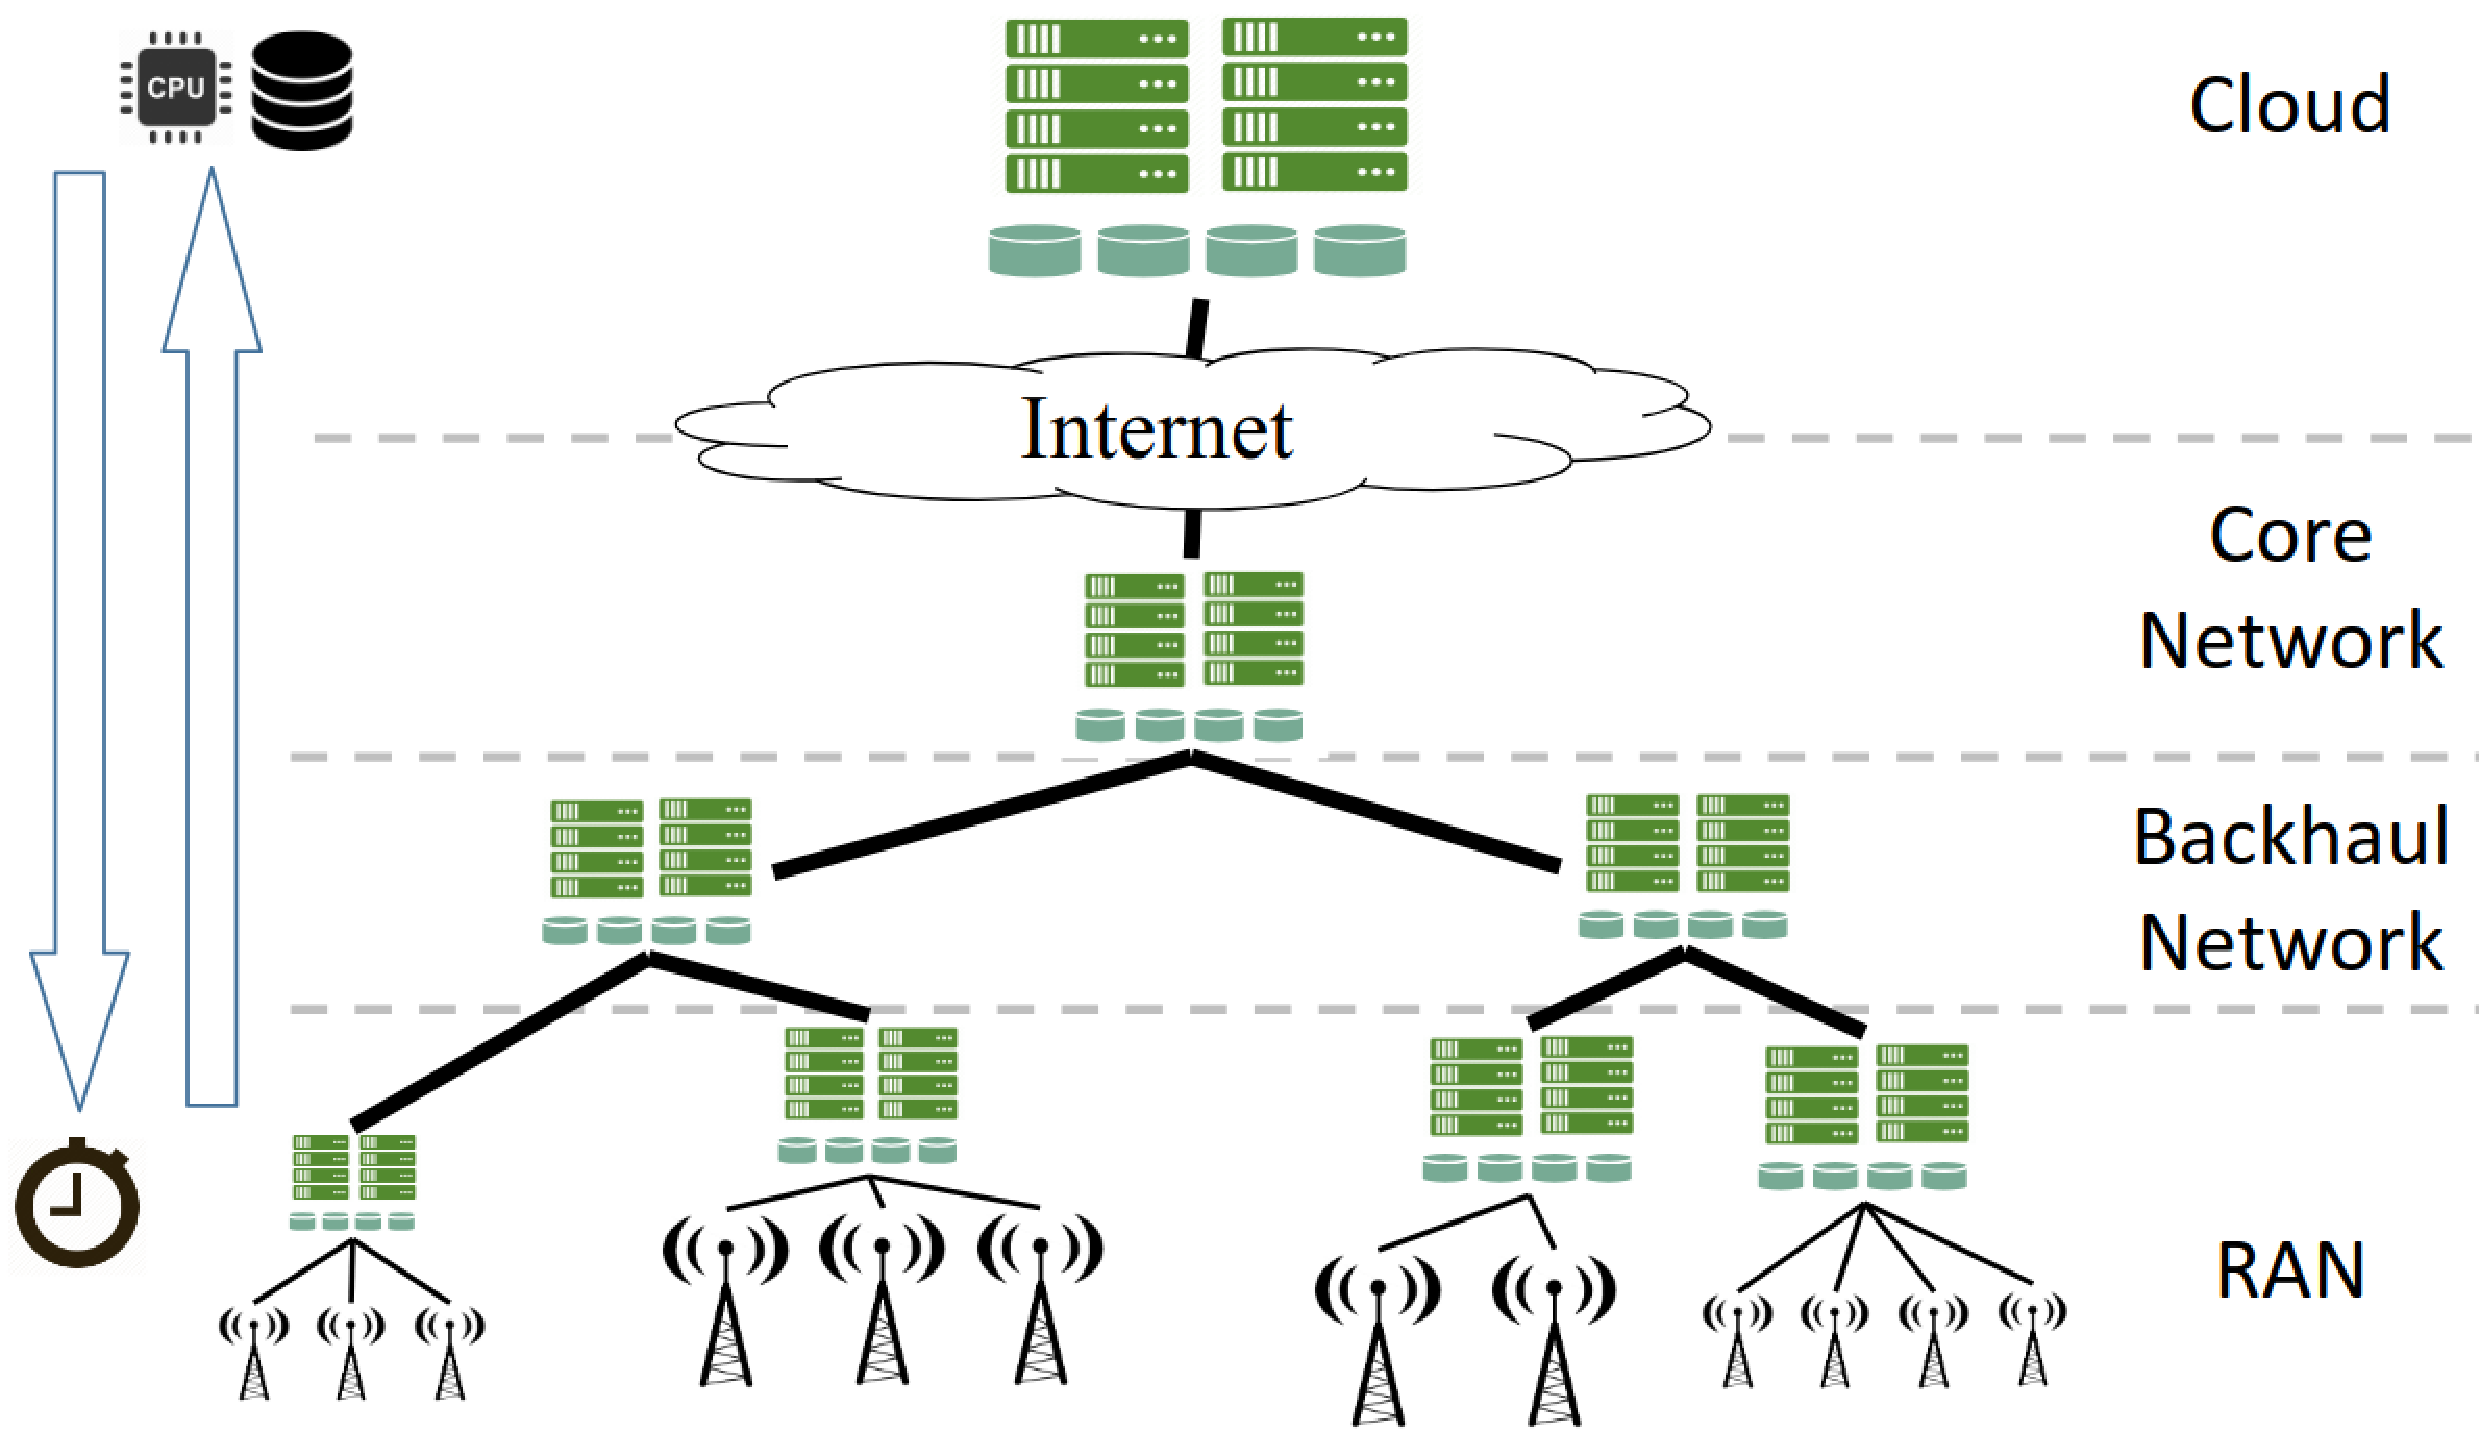
\includegraphics[width=0.9\linewidth]{img/5g/mec}
\end{center}
Si hanno risorse ad ogni livello (Cloud Edge Continuum), ovviamente con limitazioni su applicazioni contenute e capacità disponibile.\\

Le domande sono: 
\begin{itemize}
	\item Dove installare i vari moduli? Cloud? MEC server? Dispositivo stesso? 
	\item Come viene gestita la mobilità dei dispositivi che utilizzano il servizio?
\end{itemize}
La risposta dipende dai requisiti del modulo e dei link di comunicazione tra moduli.\\

Vantaggi: 
\begin{itemize}
	\item Architettura fortemente decentralizzata e localizzata
	\item Riduzione della latenza e jitter end-to-end
	\item Riduzione traffico verso il core della network
	\item Miglior support a Servizi Location/Context-Aware
\end{itemize}

\newpage

Sfide: 
\begin{itemize}
	\item Integrazione nella rete: Come coesistono MEC e standard 3GPP? Come garantisco la trasparenza a UE?
	\item Portabilità delle applicazioni MEC, Allocazione e de-allocazione trasparenti ed impercettibili (seamless); Architetture HW e SW standard e open
	\item Sicurezza; Come garantisco isolamento tra le VM nei MEC server? Come controllo dinamicamente l'uso corretto delle risorse
	dell'operatore?
	\item Performance; Dimensionamento delle VM; Allocazione ottimizzata delle VM all'interno della rete
	\item Resilienza
\end{itemize}

\subsection{Network Slicing}

Network slicing è un concetto che trasforma la rete/sistema  da \textbf{paradigma} statico ad uno \textbf{dinamico} (nei primi standard si avevano qualità di servizio predefinite, qualunque fosse il servizio), nel quale \textbf{reti logiche} vengono create \textbf{on demand} con risorse e topologie ottimizzate per servire uno scopo specifico, una categoria di servizi o singoli utenti.\\

\textbf{Network Slice Instance} è un insieme di network function e risorse di rete organizzate e configurate per fornire una rete logica che soddisfa certe caratteristiche.\\

Per ogni classe di servizio/esigenza viene costruito un overlay di rete ad hoc al di sopra della rete fisica. Diventa molto più flessibile la gestione della rete \textit{al servizio di un servizio}, viene creata una slice della rete ad hoc per il servizio.\\

5G abbandona l'idea degli standard precedenti in cui \textit{one size fits all}, si hanno diversi casi d'uso e le risorse vengono allocate di conseguenza. \\

%End L20

\newpage

\subsection{Architettura}

\subsubsection{LTE CUPS (Control User Plane Separation)}

Un po' di "storia": due release prima di 5G effettivo (Rel-14, 5G è la 16, quindi si parla ancora di LTE, anche se 6 release dopo). 
\begin{center}
	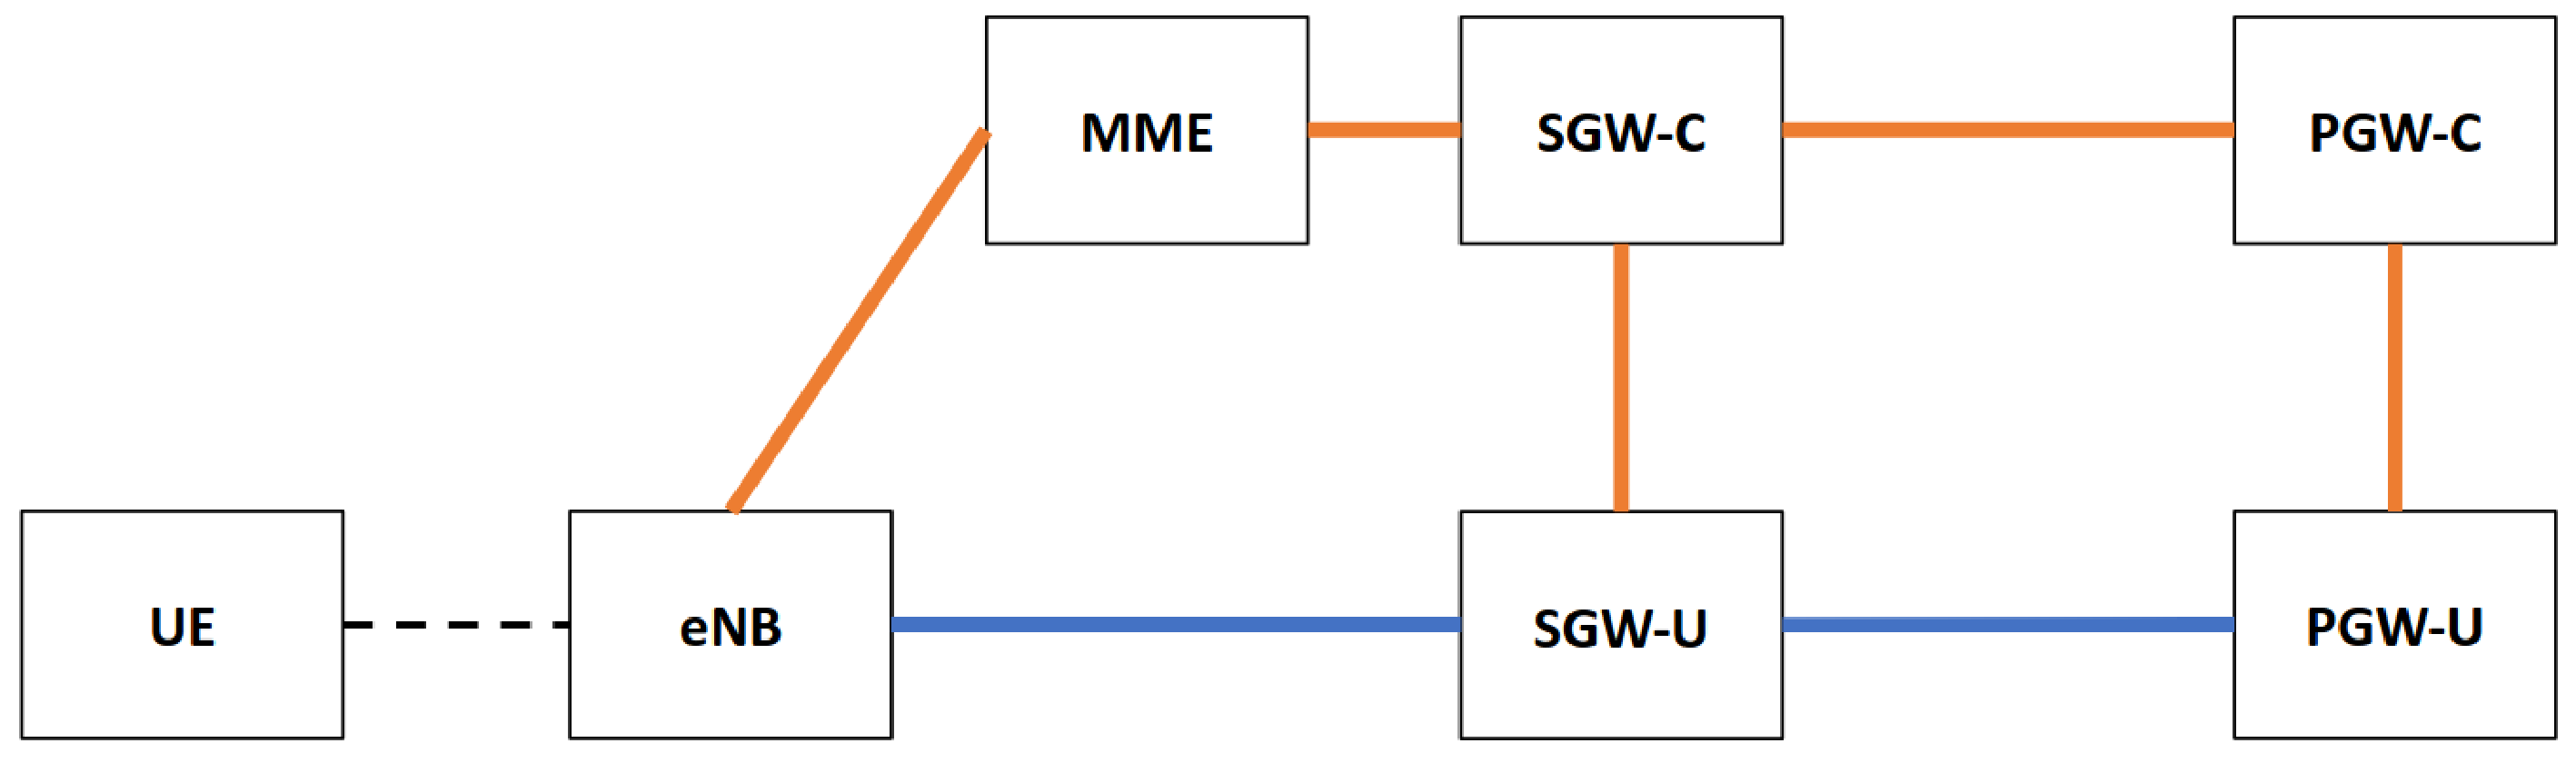
\includegraphics[width=0.7\linewidth]{img/5g/ltecups}
\end{center}
Si ha una \textbf{separazione} tra \textbf{user plane e control plane} in modo che siano indipendenti l'una dall'altra, permettendo una migliore scalabilità, indipendente tra piano dati e piano di controllo (ognuno dei due piani può essere scalato senza che l'altro vada necessariamente modificato). \\

\subsubsection{Divisione dei Plane}
In 5G, rispetto le versioni precedenti, si ha un data plane semplificato quasi all'estremo (un solo componente che si occupa del controllo), mentre il control plane prevede una sempre maggior divisione dei compiti su componenti diverse.
\begin{center}
	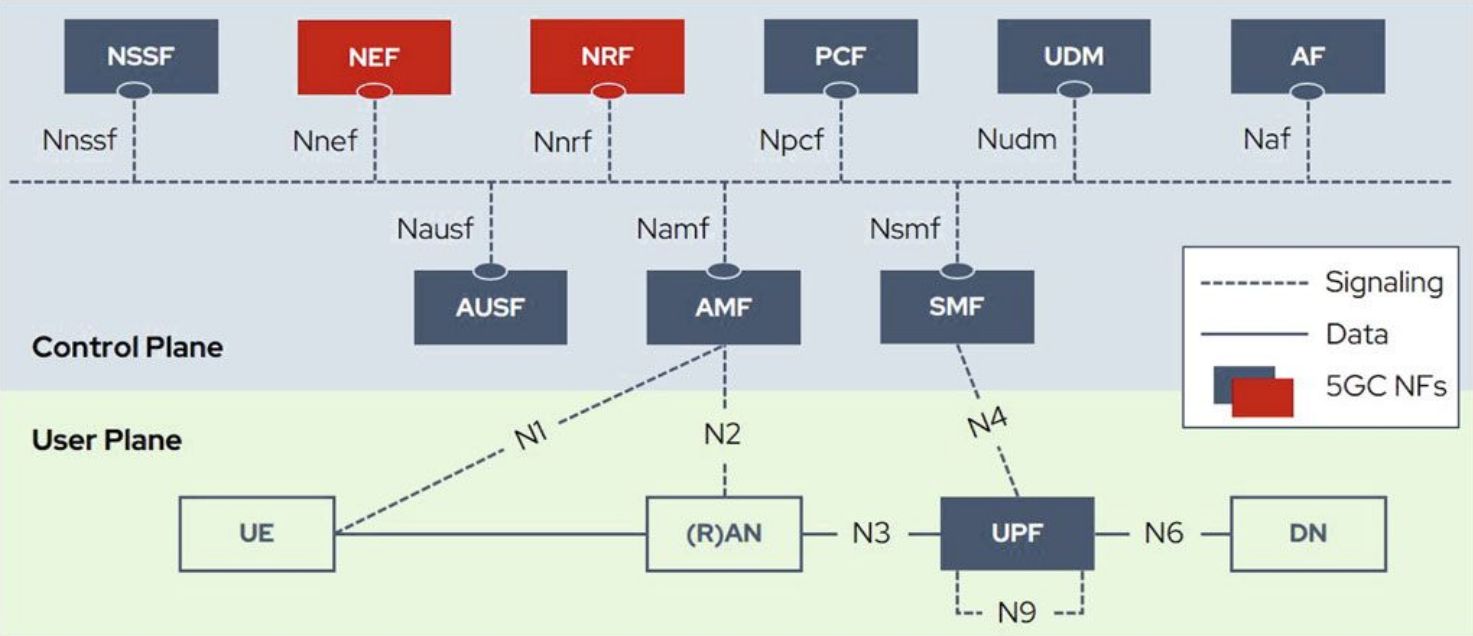
\includegraphics[width=0.9\linewidth]{img/5g/arch}
\end{center}

Per la parte di comunicazione all'interno del data plane e tra i due piani rimane una comunicazione punto-punto tra i vari componenti. Invece, all'interno del control plane viene usata una \textbf{service-based architecture} con un \textbf{modello publish-subscribe}: ogni componente è una VNF ed ognuna di queste implementa un servizio con API REST. Ogni VNF può consumare una o più API delle altre VNF. Si ha un bus comune di comunicazione tra tutte le VNF.\\

Ogni componente del control plane è una VFN, quindi ognuno può evolvere indipendentemente, ogni VNF può essere (dis)attivata o scalata in base alla necessità. Ci sono tanti "micro-servizi" che svolgono le funzioni precedentemente svolte dal control plane.\\

\paragraph{Control Plane: } All'interno del control plane si trovano
\begin{itemize}
	\item \textbf{NRF Network Repository Function}: permette od ogni servizio di registrarsi e rendersi individuabile dalle altre VNF
	
	\item \textbf{AMF Access \& Mobility Management Function}: gestisce la maggior parte del traffico di segnalazione per autenticazione, registrazione e mobilità; una delle 3 parti in cui è stato diviso l'MME, gestisce una parte delle funzionalità precedentemente svolte dall'MME ma non gestisce dati di sessione (compito dell'SMF)
	
	\item \textbf{SMF Session Management Function}: Gestisce il controllo relativo alla creazione di sessioni dati; permette di creare delle sessioni user plane; unico che comunica con l'unica funzionalità core del data plane (ovvero la User Plane Function UPF)
	
	\item \textbf{UDM Unified Data Management Function}: fornisce un front-end unico per tutti i dati che ciascuna funzionalità di rete può richiedere; ogni NF può aver bisogno di dati diversi (strutturati, non-strutturati, semi-strutturati); qualsiasi NF che richiede un qualche tipo di database effettua le richieste di dati qua
	
	\item \textbf{PCF Policy Control Function}: effettua la parte di gestione e controllo delle politiche di accesso/mobilità in rete e di utilizzo dello user plane (prima dato alle PCRF)
	
	\item \textbf{AUSF Authentication Server Function}: gestisce tutto ciò che riguarda l'autenticazione e la generazione delle chiavi di cifratura
	
	\item \textbf{NSSF Network Slice Selection Function}: la funzione che dice quale può essere la slice migliore e consentita per un determinato servizio richiesto da un determinato utente
	
	\item \textbf{NEF Network Exposure Function e AF Application Function}: per integrare e permettere di utilizzare più informazioni; la NEF espone all'esterno della rete delle funzionalità, la AF permette all'applicazione di rendersi visibile all'interno della rete core; permettono alla rete e alle applicazioni/servizi esterni di dialogare tra loro esponendo funzionalità
\end{itemize}


\paragraph{User Plane:} Semplificato, rispetto alle release precedenti: 
\begin{itemize}
	\item \textbf{UE User Equipment}
	\item \textbf{RAN}: composta da gNodeB (per distinguerla dalle precedenti principalmente), gestisce la parte radio (link allo UE)
	\item \textbf{UPF User Plane Function}: unica componente dello user plane, si occupa dell'inoltro dei pacchetti utente da/verso l'esterno (DN); il loop con interfaccia N9 permette routing tra da data network
	\item \textbf{DN Data Network}: rete esterna
\end{itemize}

\paragraph{Protocol Data Unit PDU:} I pacchetti utente viaggiano all'interno di una connessione end-to-end sullo user plane chiamata PDU session. La sessione va da uno UE a uno specifico DN. Connessione dal device alla rete esterna (DN). Al di sopra di ha il livello applicativo, al di sotto uno stack (idealmente) IP-MAC-PHY.\\

Lo stack di protocolli lato user plane rimane simile a quello 4G (con le necessarie modifiche per la PDU).

\paragraph{Multiple PDU Sessions:} Un singolo UE può avere più connessioni attive, verso diverse data network, attraverso diverse UPF. Viene utilizzata una UPF per ogni collegamento.

\paragraph{Interfaccia N9:} Permette di connettere tra loro più UPF e fare routing verso altre data network. Per fare ciò si usa un ulteriore UPF che classifica il traffico in downlink: chiamata \textbf{ULCL (UpLink CLassifier)}, questa viene configurata apposta per classificare il traffico in uplink di ciascun dispositivo, permettendo di fare routing verso la corretta Data Network in modo trasparente all'utente.\\

\newpage

\subsubsection{Network Slices}

Si espandono le funzionalità dei TTF in 4G, i quali permettevano \textit{solo} la configurazione di alcuni parametri di rete. Le \textbf{Network Slices 5G} permettono di \textbf{classificare diversi casi d'uso} e per ciascuno si hanno diversi siti (a livello di distanza rispetto all'utente)
\begin{center}
	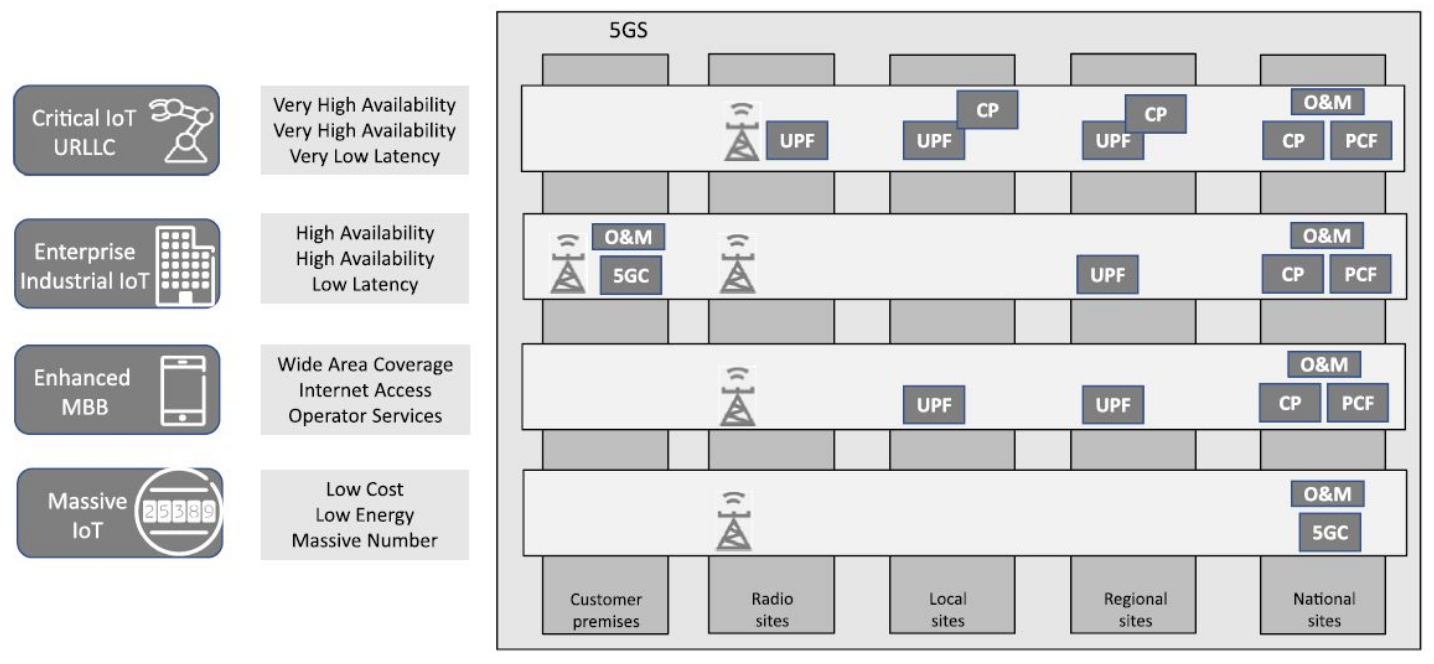
\includegraphics[width=0.97\linewidth]{img/5g/slicing}
\end{center}

Permette non solo di stabilire le \textbf{caratteristiche del servizio}, ma specifica anche la \textbf{composizione delle NF che permettono il servizio}. Rende possibile avere anche più livelli di Control Plane CP, per diversi servizi all'interno dello stesso caso d'uso (un servizio magari necessita di tempi di risposta molto brevi, ma non tutti); l'uscita dalla rete può essere prevista in diversi punti in base al servizio (vedi Critical IoT URLLC). I servizi sono "confezionati" anche a livello di collegamenti logici tra NF.\\

Fornisce grande flessibilità alla rete oltre che alla qualità di servizio, tutto questo grazie alle tecnologie di virtualizzazione.\\

\newpage

\paragraph{Identificazione:} Per l'identificazione della slice si usa uno slice identifier a 32 bit
\begin{center}
	\begin{tabular}{| C{2cm} | C{6cm} :}
		\multicolumn{2}{c}{Single-Network Slice Selection Assistance Information (S-NSSAI)} \\
		\cline{1-1} \cdashline{2-2}
		Slice Service Type (SST) \newline 8 bits & Slice Differentiator (SD) 24 bits \\
		\cline{1-1} \cdashline{2-2}
	\end{tabular}
\end{center}

I primi 8 bit indicano l'utilizzo per cui è pensata la network slice: 
\begin{center}
	\renewcommand{\arraystretch}{1.6}
	\begin{tabular}{| C{1.3cm} | C{1.2cm} | C{8.5cm} |}
		\hline
		0  & & Reserved \\
		\hline
		1  & eMBB & suitable for handling of 5G Enhanced Mobile Broadband \\
		\hline
		2  & URLLC & suitable for handling of Ultra-Reliable Low Latency Communications \\
		\hline
		3  & MIoT & suitable for handling of Massive IoT \\
		\hline
		4  & V2X & suitable for handling of V2X services \\
		\hline
		5-127  & & Reserved \\
		\hline
		128-255  & & Operator-specific \\
		\hline
	\end{tabular}
\end{center}
Mentre gli ultimi 24 definiscono la specifica istanza di un determinato tipo. \\

La slice consentita all'utente viene determinata con il dialogo tra UE + AMF + NSSF + UDM. In questo modo il dispositivo è a conoscenza della slice a cui è assegnato e metterà l'identificativo della slice all'interno dei pacchetti.\\

\subsubsection{5G e MEC}

L'integrazione tra 5G e MEC avviene tramite UPF come data plane nell'architettura MEC. UE che usa un servizio MEC ha UPF (PSA) collegato alla MEC platform dove è attivo il servizio che utilizza.\\

\subsubsection{5G RAN - 5G NR (New Radio)}

Vogliamo mantenere i 14 simboli OFDMA ma lo slot da 10ms non va bene, si vuole ridurre la latenza. La soluzione è \textbf{ridurre la durata dei simboli} (stesso numero, mento tempo), risparmiando banda.\\

Lo standard 5G NR definisce 5 diverse durate, indicate come \textbf{numerology}. Definisce anche due possibili intervalli di frequenze:
\begin{itemize}
	\item \textbf{FR1 (Frequency Range 1)}: 410MHz - 7125MHz
	\item \textbf{FR2 (Frequency Range 2)}: 24250MHz - 52600MHz
\end{itemize}

Di conseguenza, per una numerology $\mu$ si ha una $\Delta f$ (distanza tra le frequenze) calcolabile come
$$ \Delta f = 2^\mu \cdot 15 [kHz] $$
\begin{center}
	\begin{tabular}{| C{1.5cm} | C{2cm} | C{3cm} | C{2cm} | C{2cm} |}
		\hline
		$\mu$ & $\Delta f$ & Cyclic Prefix & Banda di frequenza & Utilizzo  \\
		\hline
		0 & 15 & Normal & FR1 & Dati \\
		\cline{1-4}
		1 & 30 & Normal & FR1 & e \\
		\cline{1-4}
		2 & 60 & Normal, Extended & FR1 \& FR2 & Controllo \\
		\cline{1-4}
		3 & 120 & Normal & FR2 & \\
		\hline
		4 & 240 & Normal & FR2 & Controllo \\
		\hline
	\end{tabular}
\end{center}

Quando aumenta la distanza tra le portanti si usa solo il secondo range di frequenze, considerevolmente più ampio, altrimenti non ci starebbero abbastanza utenti all'interno. Per formare un Resource Block con 21 subcarrier servono, in base alla numerology, un range di
\begin{center}
	\begin{tabular}{ c | c | c | c | c | c}
		$\mu$ & 0 & 1 & 2 & 3 & 4 \\
		\hline
		& 180kHz & 360kHz & 720kHz & 1,44MHz & 2,88MHz 
	\end{tabular}
\end{center}

Raddoppiare la banda permette di dimezzare il tempo necessario per ogni simbolo. All'interno dello scheduling si possono allocare resource block con numerology diverse, magari anche in base alla slice utilizzata. Oltre alla rete, anche la configurazione della radio si può adattare all'utilizzo (se richiede latenza bassa si aumenterà la banda e diminuirà la durata del simbolo).\\

\newpage

%TODO: Da rivedere, non nell'esame
%\subsection{Open-RAN O-RAN}
%
%Rientra nello standard. Prevede separazione tra 
%* Central Unit CU
%* Distributed Unit DU
%* Radio Unit RU
%%compl, idk s109
%
%La parte interessante sono i controller al di sopra, che sono programmabili e gestibili dall'utente. Dialogano con le varie componenti. \\
%
%I blocchi blu sono standard 5G (3GPP), O-RAN aggiunge sulla BS una parte programmabile e ottimizzabile, anche con tecniche ti AI/ML, il tutto svolgibile direttamente sulla BS.\\

%Un saaacco di cose da rivedere, non vedo l'ora
%End L22
    
    % !TeX spellcheck = it_IT
\section{Comunicazione Satellitare}

\subsection{Geometria del link satellitare}

\paragraph{Piano orbitale:} Il "cerchio" secondo cui il satellite si muove, generalmente indicato tramite l'inclinazione rispetto all'equatore.

\paragraph{Angolo di Azimuth:} Orientamento rispetto al nord geografico, in senso orario dice dove orientare la stazione di terra per poter ricevere il segnale; vogliamo capire come orientare l'antenna per ricevere o trasmettere nella maniera migliore possibile.

\paragraph{Angolo di elevazione:} Angolo rispetto all'orizzonte; quanto "alzare" il ricevitore.

\paragraph{Angolo di copertura:} Porzione di superficie terrestre visibile da satellite (angolo tridimensionale); quanto terreno copre un satellite, più è lontano maggiore sarà questo angolo.

\paragraph{Lunghezza fisica del link:} Bisogna tenere in conto della distanza dal satellite, in quanto significativa per i tempi di trasmissione, e questa varia in base alla posizione del satellite: sarà minima quanto il satellite è direttamente sopra il ricevitore, sarà massima quando il satellite è all'orizzonte; questo porta ad un variare del tempo di propagazione (elevato jitter) durante la durata di connessione al satellite. 

\paragraph{Attenuazione in funzione dell'angolo di elevazione:} Un angolo di elevazione molto basso (verso l'orizzonte, link molto lungo) porta a far perdere energia alla trasmissione.

Inoltre, l'attenuazione dipende anche dalla condizione atmosferica, variando, anche significativamente, l'assorbimento del segnale. Ne va tenuto conto durante il calcolo del path loss.

\begin{center}
	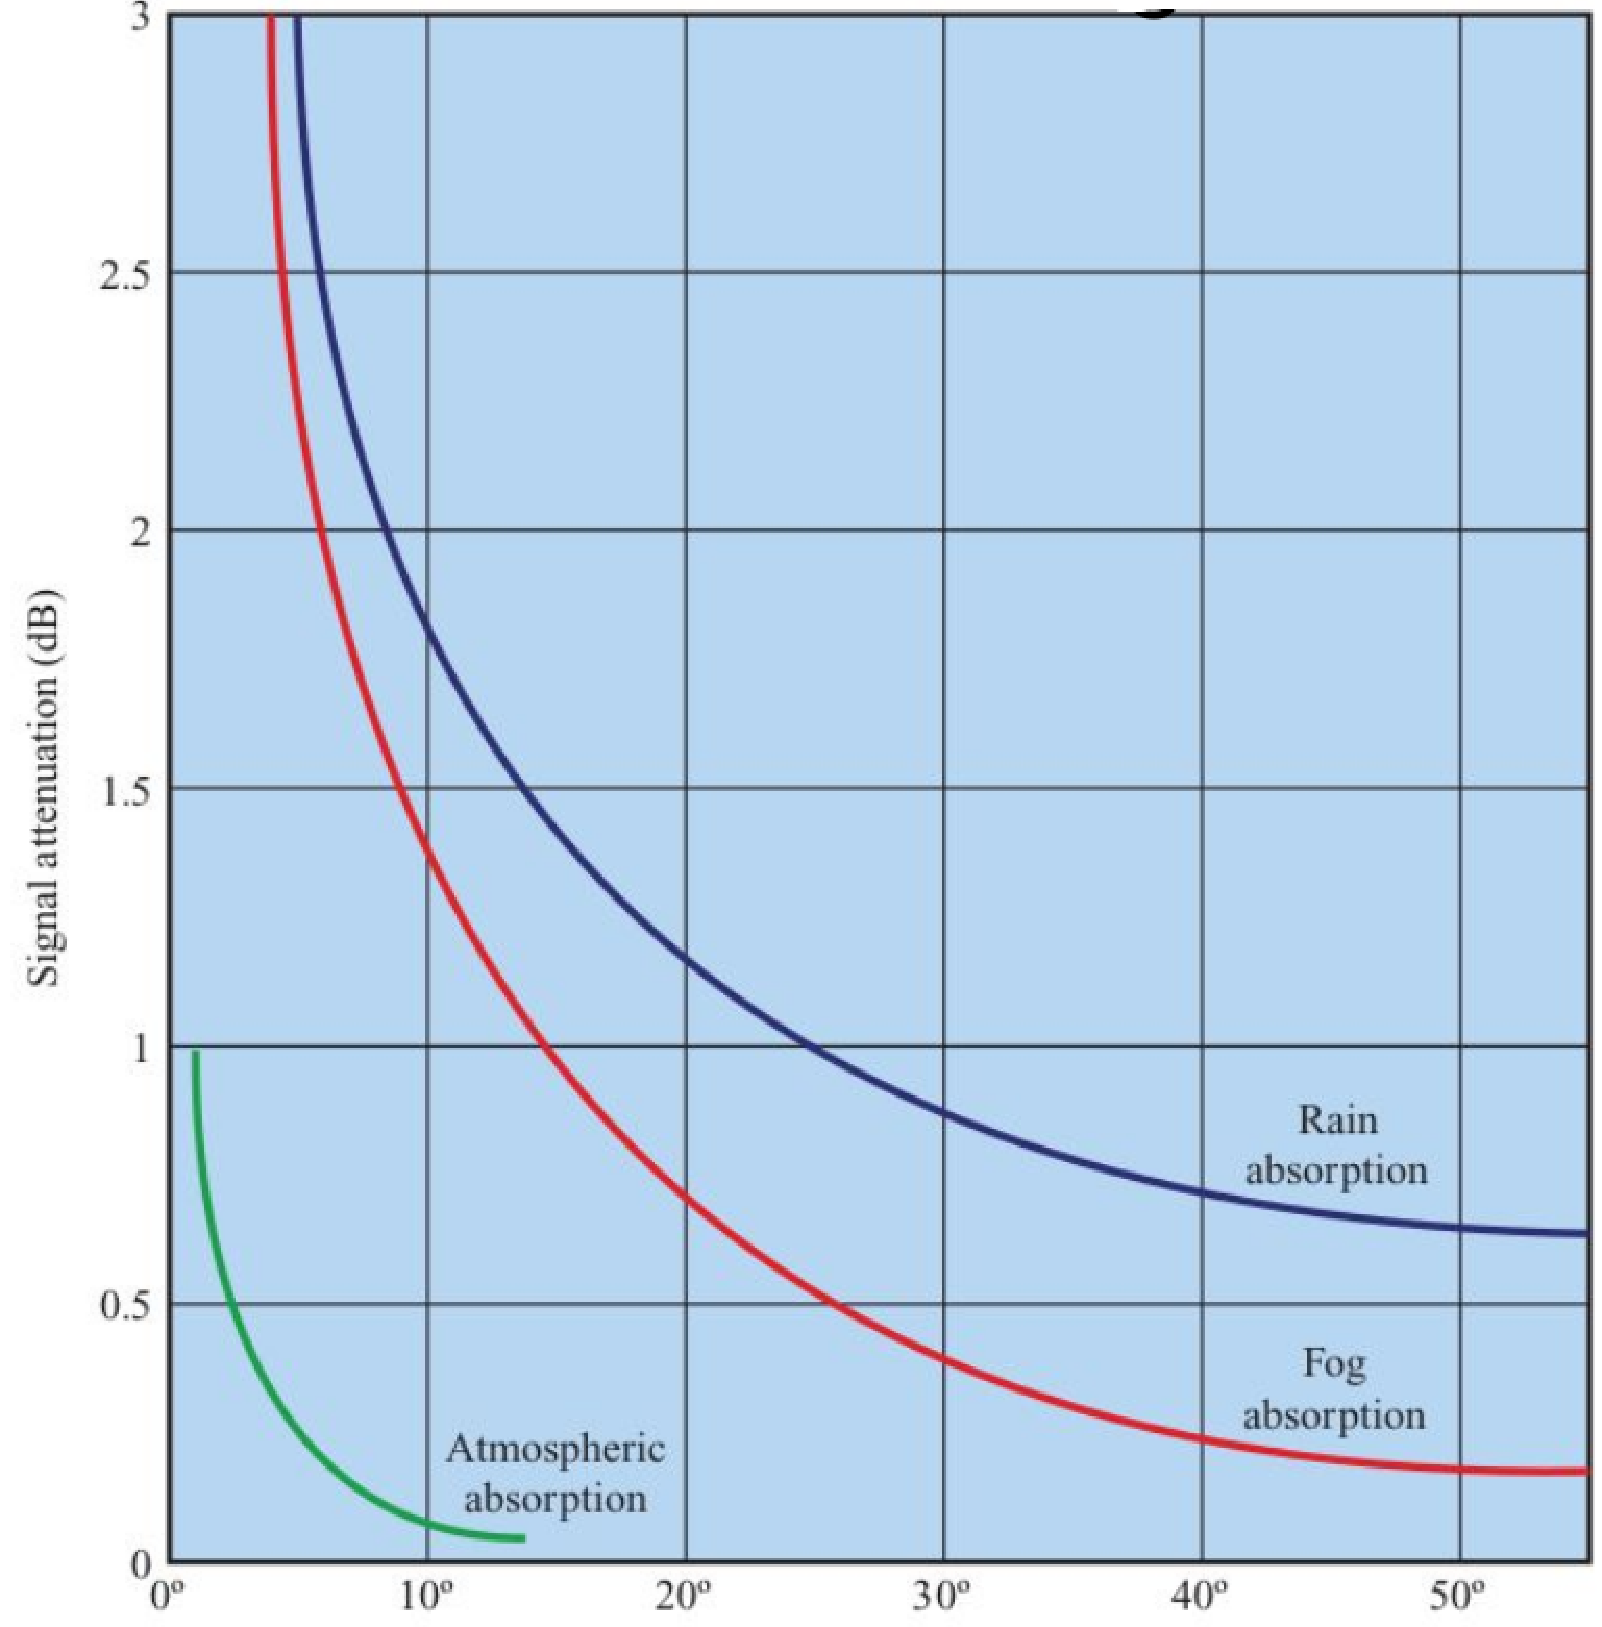
\includegraphics[width=0.55\linewidth]{img/sat/atten}
\end{center}

%Controlla dettagli
\subsection{Orbite}

\subsubsection{Geostationary Earth Orbit GEO}

Orbita geostazionaria:
\begin{itemize}
	\item periodo dell'orbita: 24h
	\item visibilità: permanente
	\item angolo di elevazione: fisso
	\item elevata copertura: 3 satelliti separati da 120$^\circ$ coprono la maggior parte delle zone abitate
	\item qualità del segnale bassa a causa della distanza
	\item elevato delay, $\sim 250ms$
\end{itemize}

A circa 35786km di altezza, un satellite ruota alla stessa velocità della Terra, quindi da una prospettiva "sul terreno", il satellite appare in posizione fissa. Questo permette di usare antenne fisse, riducendo costi e complessità a terra, ed allo stesso tempo avere una copertura molto elevata (sono lontani, "vedono" molto).\\

\subsubsection{Low Earth Orbit LEO}

Orbita più vicina alla terra: 
\begin{itemize}
	\item periodo dell'orbita: 1.5-2h
	\item visibilità per passaggio: 15/20 minuti prima che scompaia all'orizzonte
	\item RTT: alcuni ms
	\item copertura: 6000km
	\item ridotto delay per via dell'orbita più bassa
	\item minore potenza di trasmissione e migliore utilizzo dello spettro
	\item La comunicazione tra stazioni terrestri spesso coinvolge più hop tra satelliti (handoff)
	\item garantire la copertura 24/24 richiede un "elevato" numero di satelliti
\end{itemize}

Sempre più rilevanti, in particolare per applicazioni di comunicazione. Sono posizionati a quota tra 160 e 2000km e sorvolano aree diverse ad ogni passaggio, con una copertura relativamente limitata. I vantaggi sono una bassa latenza e una minor potenza di trasmissione richiesta, al costo di una copertura limitata, di conseguenza richiedendo grandi costellazioni, e una gestione più complessa per gestire tracciamento, handover e comunicazione tra satelliti.\\

\subsubsection{Medium Earth Orbit MEO}

Via di mezzo tra LEO e GEO:
\begin{itemize}
	\item periodo dell'orbita: 5-10 ore
	\item visibilità per passaggio: 2-8 ore
	\item RTT: decine di ms
	\item copertura: 12000 - 15000 km
	\item minori handoff rispetto a LEO
	\item maggiore delay e potenza di propagazione rispetto a LEO, ma significativamente inferiore rispetto a GEO
\end{itemize}

Usato da Global Navigation Satellite System GNSS. RTT, visibilità per passaggio e periodo dell'orbita dipendono (ovviamente) dall'altezza del satellite (abbastanza variabile in questa categoria).

%Linka simulatore traccia terreste dalle slide?

\subsubsection{Costellazione}

Soprattutto nelle orbite LEO e MEO, sono richiesti più satelliti per una copertura continua e globale (o regionale). Le costellazioni differiscono per numero di piani orbitali e numero di satelliti. La progettazione della costellazione dipende dai requisiti che si vogliono soddisfare.

\subsection{Architettura}
Sono presenti 3 segmenti:
\begin{itemize}
	\item \textbf{Space} segment
	\item \textbf{Ground} segment
	\item \textbf{User} segment
\end{itemize}

\begin{center}
	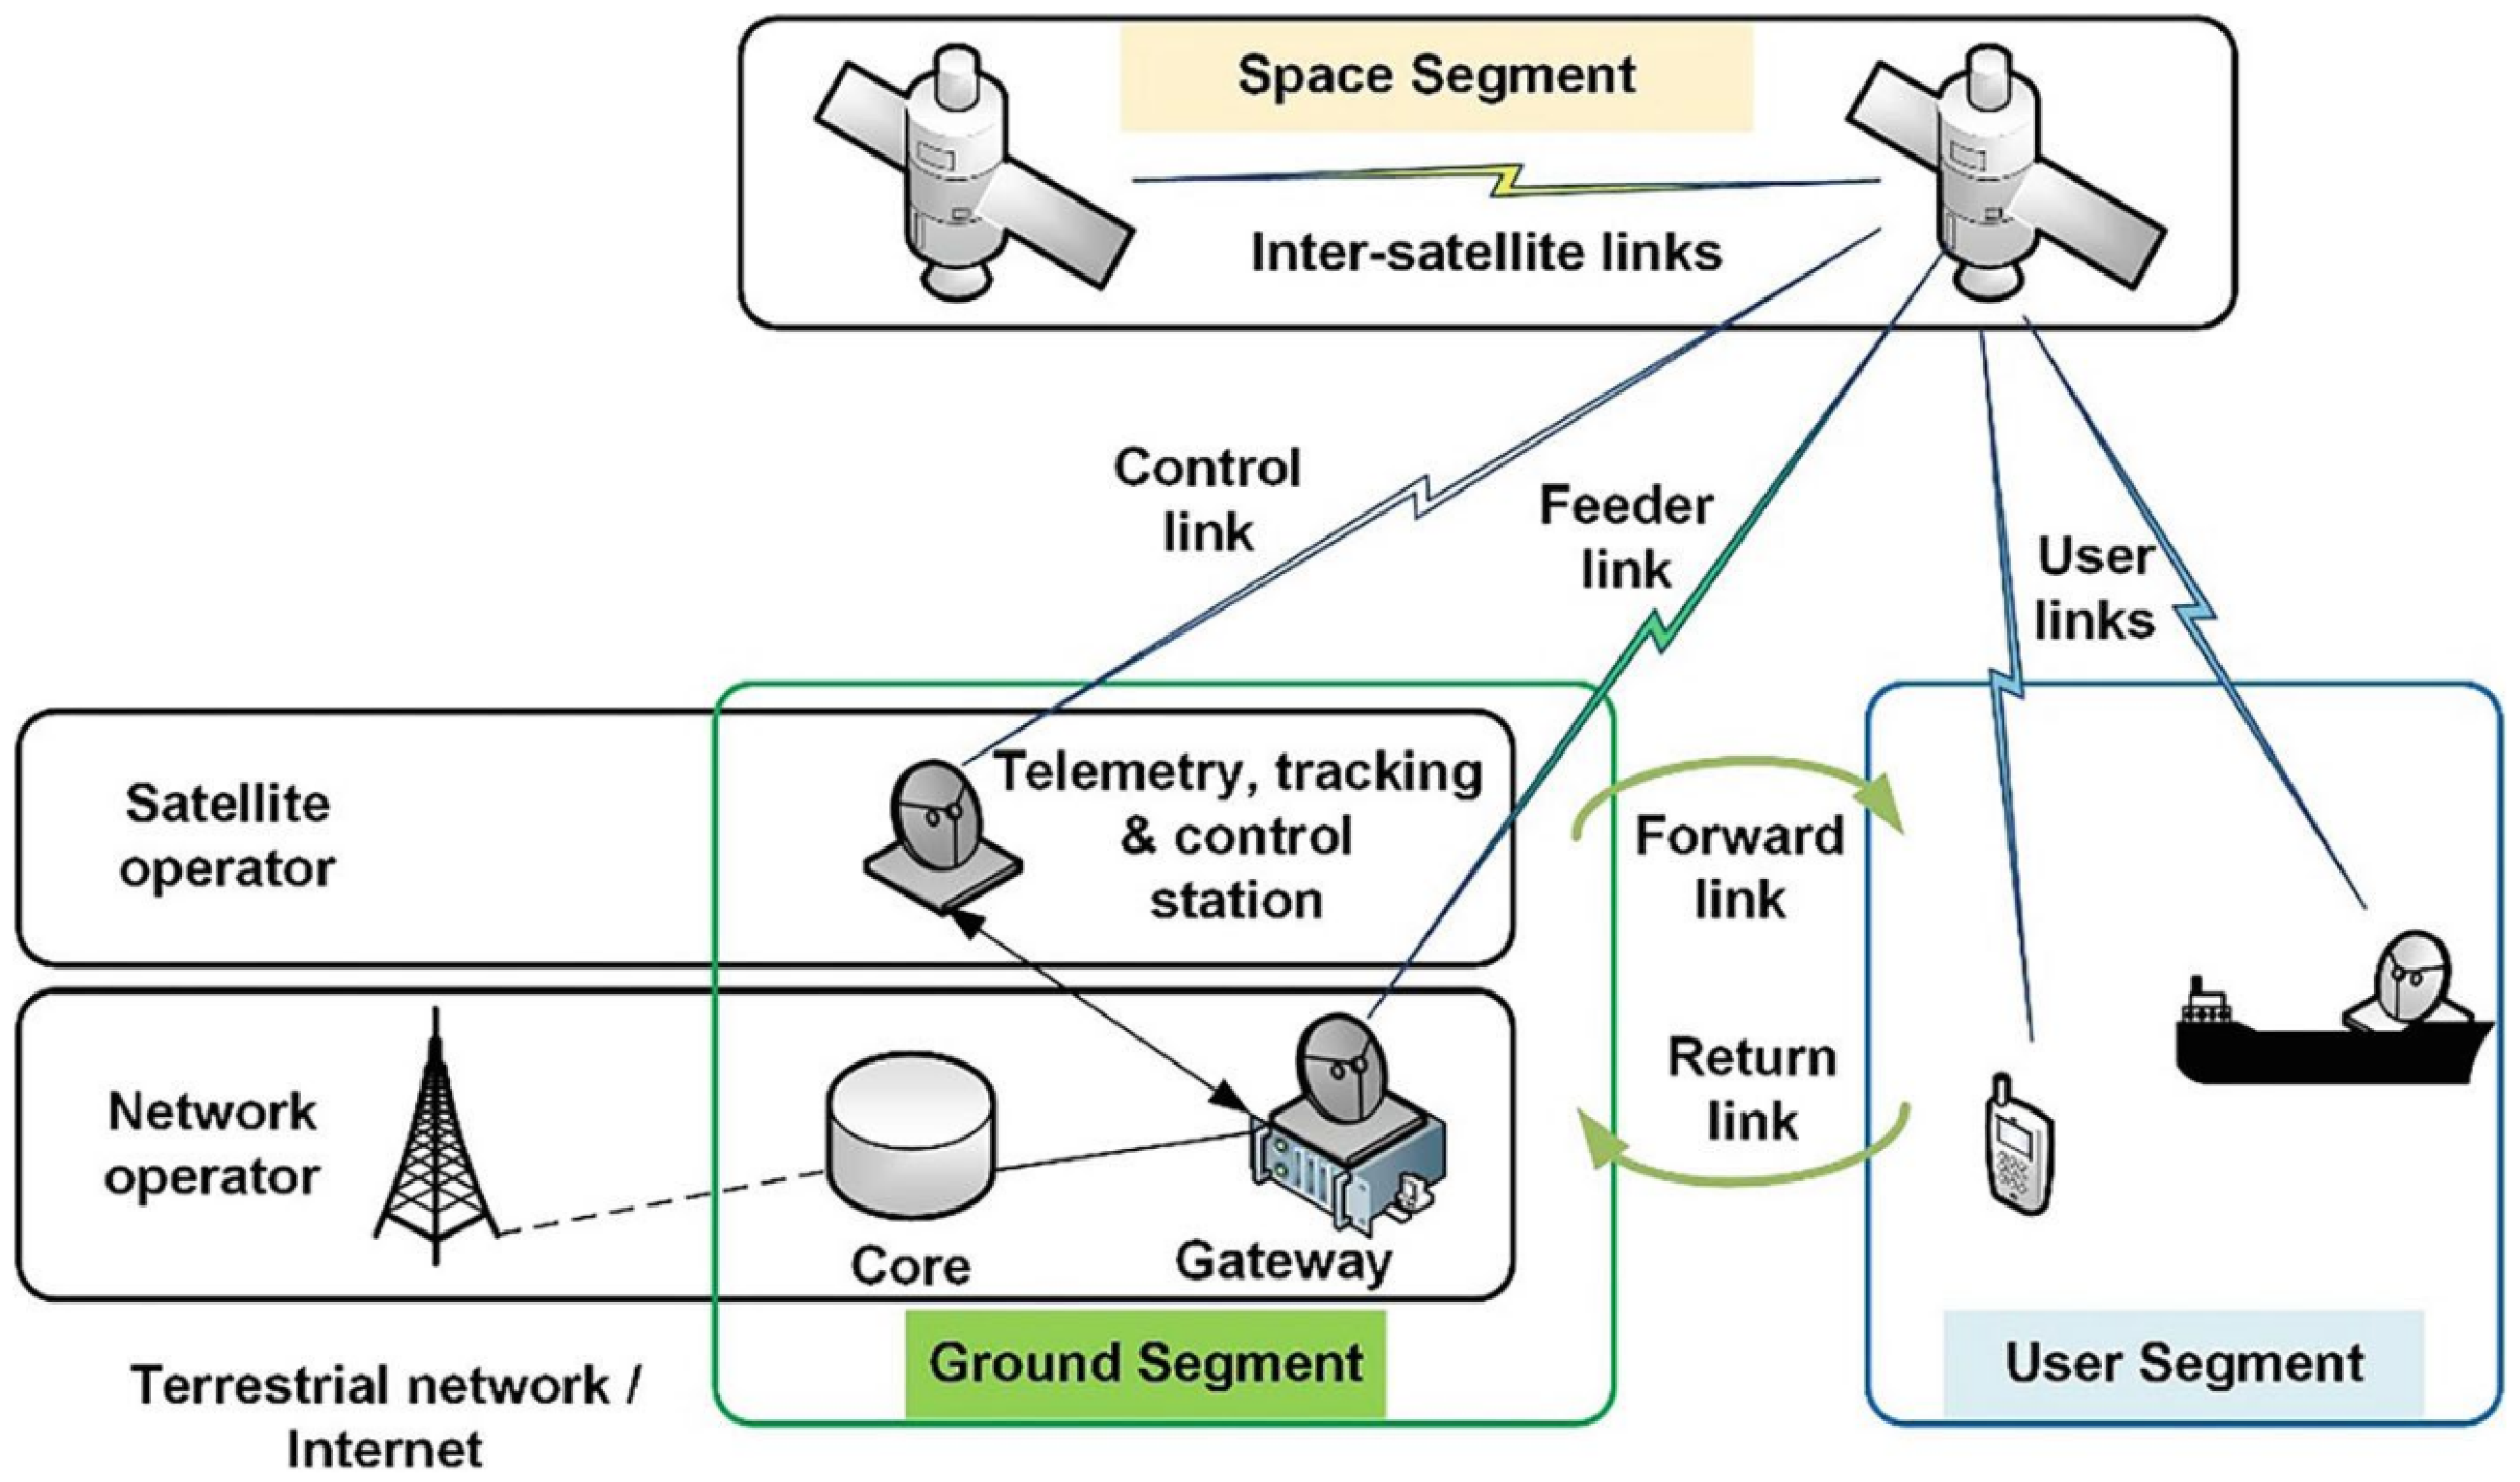
\includegraphics[width=0.7\linewidth]{img/sat/arch}
\end{center}

\paragraph{Space segment:} Contiene i satelliti e le relative costellazioni, con anche la possibilità di avere link inter-satellitare (tramite radio o anche ottici, via laser).

\paragraph{Ground segment:} Contiene la "parte di controllo" del sistema, include il gateway, ovvero ciò che connette le stazioni di terra con i satelliti, oltre che le stazioni di terra e tutto ciò che riguarda controllo, telemetria e tracking.

\paragraph{User segment:} Ovvero gli utenti, utilizzatori dei servizi, possono essere mobili o fixed.

\subsubsection{Allocazione frequenze}
\begin{center}
	\resizebox{\textwidth}{!}{\begin{tabular}{|l|l|l|l|}
			\hline
			\textbf{Satellite band} 
			& \textbf{Frequency range} 
			& \textbf{UL or DL} 
			& \textbf{Satellite services} \\
			\hline
			\multirow{2}{*}{L band} 
			& 1525--1559\,MHz & DL 
			& \multirow{2}{*}{MSS and 5G NTN systems} \\
			& 1626.5--1660.5\,MHz & UL & \\
			\hline
			\multirow{5}{*}{S band} 
			& 1980--2010\,MHz & DL & BSS and 5G NTN systems \\
			& 2170--2200\,MHz & UL & FSS, MSS \\
			& 2500--2520\,MHz & DL & BSS \\
			& 2520--2670\,MHz & DL & FSS, MSS \\
			& 2670--2690\,MHz & UL & \\
			\hline
			\multirow{2}{*}{C band} 
			& 3.7--4.2\,GHz & DL 
			& FSS systems, good rain resilience \\
			& 5.925--6.425\,GHz & UL & \\
			\hline
			\multirow{2}{*}{X band} 
			& 7.25--7.75\,GHz & DL & FSS, MSS maritime \\
			& 7.9--8.4\,GHz   & UL & FSS, MSS \\
			\hline
			\multirow{2}{*}{Ku band} 
			& 10.7--12.75\,GHz & DL 
			& FSS, MSS and BSS systems. \\
			& 14--14.5\,GHz    & UL & \\
			\hline
			\multirow{3}{*}{Ka band} 
			& 17.3--17.7\,GHz & DL 
			& BSS and FSS systems, mobile VSAT terminals possible\\
			& 17.7--19.7\,GHz & DL & \\
			& 27.5--29.5\,GHz & UL & \\
			\hline
			\multirow{2}{*}{Q/V band} 
			& 37.5--42.5\,GHz & DL 
			& FSS systems for high throughput services \\
			& 47.2--52.4\,GHz & UL & \\
			\hline
			\multirow{2}{*}{W band} 
			& 71--76\,GHz & DL 
			& FSS system allocations, experimental missions \\
			& 81--86\,GHz & UL & \\
			\hline
	\end{tabular}}
\end{center}

\subsection{Topologie di rete}

\paragraph{Punto-punto:} Il satellite funge da ponte radio e trasmette, l'UL è da stazione a satellite, il DL da satellite a stazione (le due stazioni non si vedono ovviamente). Permette un'area di copertura molto maggiore rispetto alla rete wireless terrestre con un elevata banda, ma richiede elevata potenza di trasmissione ed ha un delay di propagazione elevato.

\paragraph{Broadcast:} Nell'ambito broadcasting viene sfruttato l'area coperta dal satellite in quanto si può usare un solo satellite per trasmettere a molteplici ricevitori. Se la parabola è correttamente orientata verso il satellite, il segnale può essere ricevuto da \textit{tanti} ricevitori.

\paragraph{Mesh:} Si vuole un link tra stazioni usando il satellite come ripetitore, non è necessario un gateway.

\paragraph{Star:} Non esistono link diretti tra stazioni , ma tutto passa tramite il gateway. Ogni stazione comunica, passando dal satellite, con il gateway, il quale provvederà a "smistare".\\

\paragraph{Hybrid:} Combina Star e Mesh, alcune comunicazioni passano attraverso il gateway ma ci sono anche link diretti tra stazioni.\\

Differenze nello scambio di messaggi:
\begin{center}
	\begin{minipage}{0.48\linewidth}
		Star topology:
		\begin{center}
			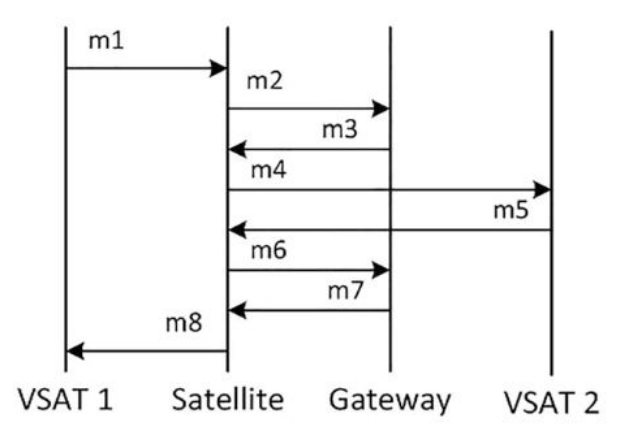
\includegraphics[width=\linewidth]{img/sat/startop}
		\end{center}
	\end{minipage}
	\hfill
	\begin{minipage}{0.48\linewidth}
		Mesh topology:
		\begin{center}
			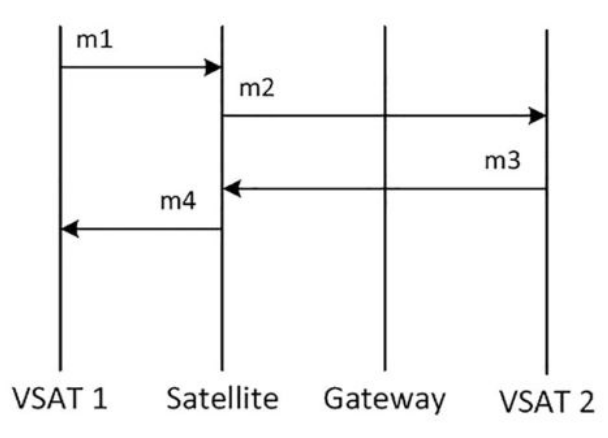
\includegraphics[width=\linewidth]{img/sat/meshtop}
		\end{center}
	\end{minipage}
\end{center}

\subsection{Medium Access Control MAC}

I protocolli MAC per le connessioni satellitari possono essere: 
\begin{itemize}
	\item \textbf{Contention-free}: FDMA, CDMA, TDMA
	\item \textbf{Contention-based Random Access}: Slotted RA, Unslotted RA
	\item \textit{Demand-based allocations with beam-hopping satellites}
\end{itemize}

\paragraph{TDMA:} Slot di tempo dedicato ad ogni trasmittente; per il downlink invece è facile, il satellite manda il pacchettone tutto assieme ed ogni ricevitore "filtra" ciò che deve leggere.

Richiede una precisa sincronizzazione tra satellite e dispositivo. Richiede un'elevata potenza di trasmissione (non tutti i dispositivi riescono). Complicato in orbite LEO a causa dell'elevata mobilità dei satelliti.

\paragraph{FDMA:} Prima modalità utilizzata per la trasmissione satellitare. Offre una minore efficienza spettrale, quindi può essere combinata con TDMA per migliorare le prestazioni.

Bisogna tenere conto dell'effetto doppler, soprattuto in orbite basse: le velocità modificano le frequenze. 

\paragraph{CDMA:} Usato dalla maggior parte dei sistemi GNSS. Soffre del Nea-far problem, molto rilevante se si considerano le distanze in ambito satellitare. Importa relativamente poco per GNSS, in quanto bisogna solo scaricare dati.

\paragraph{OFDMA:} Storicamente non molto adottato a causa dell'elevata sensibilità del sistema all'effetto doppler (richiede una certa precisione, impatta di più rispetto a FDMA).

Attualmente utilizzato dalla costellazione Starlink e dai sistemi 5G-NTN (Non Terrestrial Network).

\subsection{Integrated Satellite - Terrestrial Networks and 5G/6G NTN Technology}

Motivazioni: 
\begin{itemize}
	\item migliorare il lancio delle tecnologie 5G/6G anche in aree remote: aree rurali, aerei, navi
	\item continuità di servizio (ubiquitous connectivity): garantire connettività anche in casi di movimento "estremo", posso sempre accedere alla rete cellulare in modo trasparente all'utente
	\item migliorare l'affidabilità della rete, sia in termini di capacità che in caso di catastrofi naturali
	\item aumentare la scalabilità della rete; servizi multicast e broadcast sono difficili da implementare con protocolli unicast, con il satellitare è molto più facile
\end{itemize}

\subsubsection{Architetture possibili}

Come si può integrare la rete satellitare alla rete operatore?

\paragraph{Relay:} Satellite usato per la comunicazione, ma il relay a terra funge da ripetitore del segnale aumentando la qualità del canale. Il segnale può essere combinato BS-satellite, oppure solo relay.

\paragraph{Backhaul:} Costruire la rete di backhaul per raggiungere certe aree (gruppi di gNodeB) potrebbe essere difficile/impossibile: il satellite viene usato come rete di backhaul tra gNodeB e Core Network.

\paragraph{Direct Access:} La rete satellitare offre servizi di connettività direttamente ai dispositivi in single/dual connectivity. Il device può vedere direttamente il satellite.\\

Un esempio di connessione per utilizzi/dispositivi diversi:
\begin{center}
	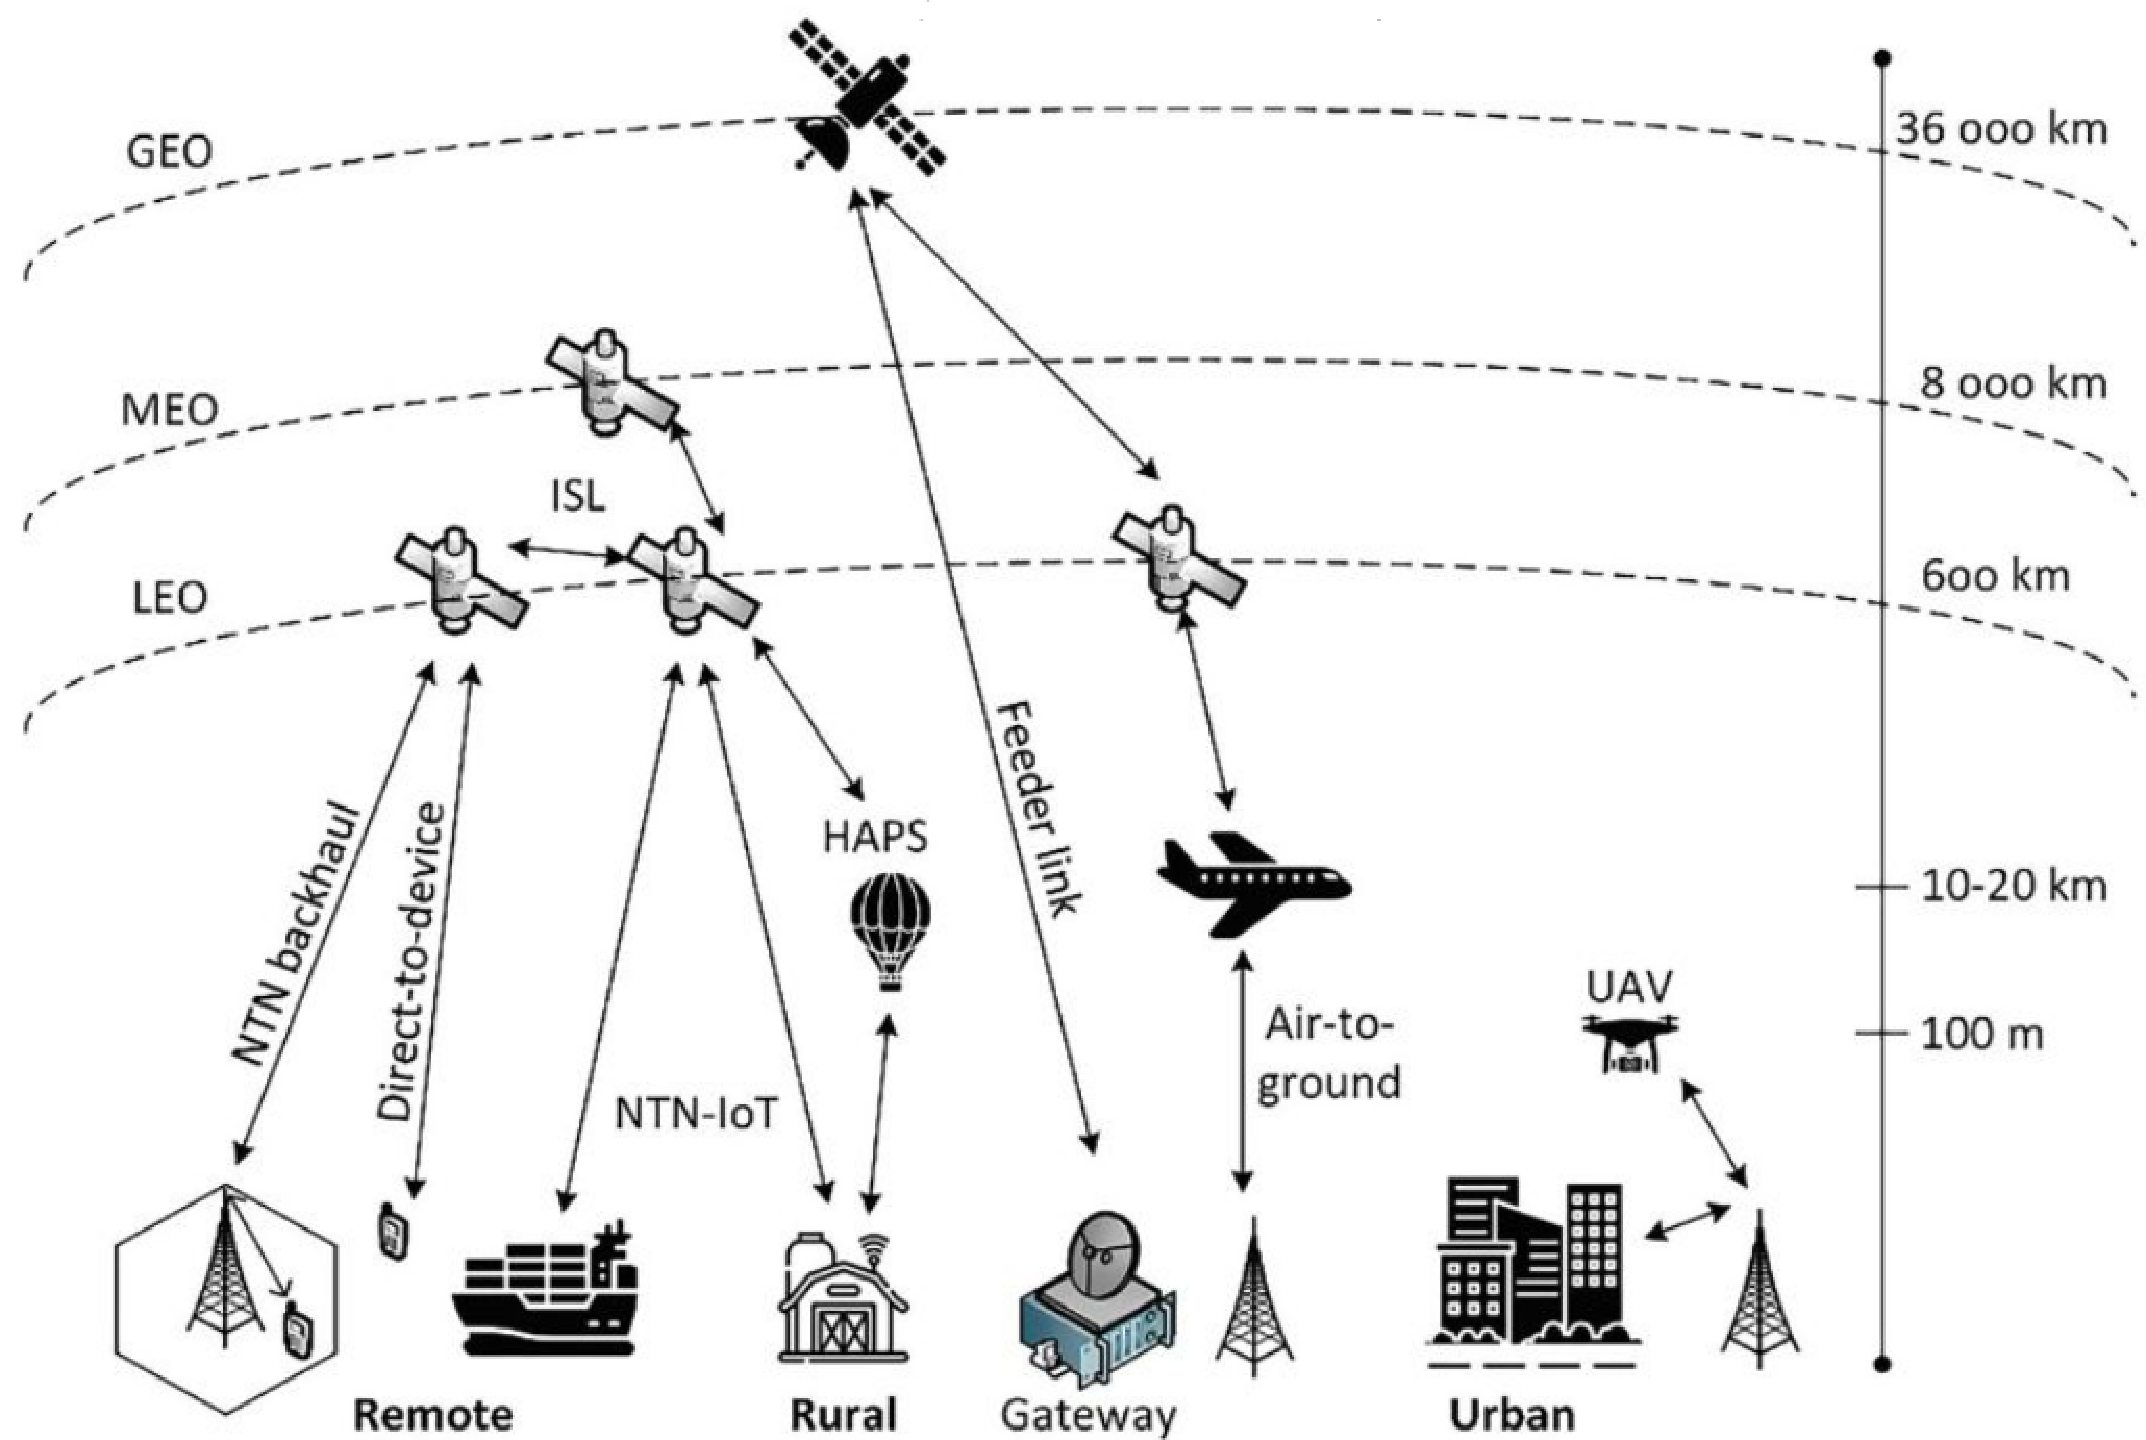
\includegraphics[width=0.75\linewidth]{img/sat/overview}
\end{center}

\subsubsection{Opzioni di integrazione}

\paragraph{NTN Transparent Payload:} Il satellite fa solo da relay, livello fisico, è il gateway che dialoga con la BS. Questa è la soluzione più semplice, adottata dalle prime release NTN. Il gateway dialoga con gNodeB (con possibili soluzioni proprietarie, non è definita la comunicazione).

\paragraph{NTN Regenerative Payload:} Il satellite implementa lo stack di una gNodeB e ne svolge le funzionalità. Permette maggiore flessibilità e utilizzo di Inter-Satellite Link ISL. Il gateway è collegato alla 5G Core. 

\paragraph{NTN Regenerative Payload with Functional Split:} Il satellite svolge solo le funzionalità del modulo distributed unit del gNodeB. I livelli di protocolli che il satellite deve implementare dipendono dall'opzione di splitting scelta dall'operatore.\\

Quindi, in breve, le opzioni per integrare la rete dal punto di visto operatore:
\begin{itemize}
	\item Semplice relay, solo processore a livello fisico
	\item tutta la BS
	\item solo la parte distribuita
\end{itemize}

% End L24
\end{document}
